% -*- Mode:TeX -*-

%% IMPORTANT: The official thesis specifications are available at:
%%            http://libraries.mit.edu/archives/thesis-specs/
%%
%%            Please verify your thesis' formatting and copyright
%%            assignment before submission. If you notice any
%%            discrepancies between these templates and the 
%%            MIT Libraries' specs, please let us know
%%            by e-mailing thesis@mit.edu

%% The documentclass options along with the pagestyle can be used to generate
%% a technical report, a draft copy, or a regular thesis. You may need to
%% re-specify the pagestyle after you \include cover.tex. For more
%% information, see the first few lines of mitthesis.cls. 

%\documentclass[12pt,vi,twoside]{mitthesis}
%%
%%  If you want your thesis copyright to you instead of MIT, use the
%%  ``vi'' option, as above.
%%
%\documentclass[12pt,twoside,leftblank]{mitthesis}
%%
%% If you want blank pages before new chapters to be labelled ``This
%% Page Intentionally Left Blank'', use the ``leftblank'' option, as
%% above. 

\documentclass[12pt,oneside]{mitthesis}
\usepackage{lgrind}
%% These have been added at the request of the MIT Libraries, because
%% some PDF conversions mess up the ligatures.  -LB, 1/22/2014
\usepackage{cmap}
\usepackage{geometry}
\usepackage{times}
\usepackage{amsmath}
\usepackage{enumitem}
\usepackage{calc}
\usepackage{siunitx} % Required for alignment
\sisetup{
  round-mode          = places, % Rounds numbers
  round-precision     = 2, % to 2 places
}
\sisetup{output-exponent-marker=\ensuremath{\mathrm{e}}}
%\documentclass{article}
\usepackage{graphicx}
% \usepackage{epstopdf}
%   \epstopdfDeclareGraphicsRule{.pdf}{png}{.png}{convert #1 \OutputFile}
%   \DeclareGraphicsExtensions{.png,.pdf}
%\includegraphics
\graphicspath{ {./figures/} }
\usepackage{caption}
\usepackage{subcaption}
\usepackage[section]{placeins}
\usepackage{siunitx}
\usepackage{booktabs}
\usepackage{geometry}
\usepackage[none]{hyphenat}
\usepackage{float}
%\usepackage[sorting=none]{biblatex}

%\usepackage{xltxtra}
\usepackage{libertine}
\usepackage{comment}
\usepackage[T1]{fontenc}
\pagestyle{plain}
\setlist[description]{leftmargin=\parindent,labelindent=\parindent}
% \geometry{left=1.in, top=.5in, right=1.in, bottom=1cm, footskip=.5cm}
\newcommand{\hg}[0]{Hg\textsuperscript{0} concentration }
\newcommand{\on}[0]{(Base ASGM = ON) simulation }
\newcommand{\off}[0]{(Base ASGM = OFF) simulation }
\newcommand{\gc}[0]{GEOS-Chem }
\newcommand{\nang}[0]{ ngm\textsuperscript{-3} }


%% This bit allows you to either specify only the files which you wish to
%% process, or `all' to process all files which you \include.
%% Krishna Sethuraman (1990).

%\typein [\files]{Enter file names to process, (chap1,chap2 ...), or `all' to process all files:}
\def\all{all}
\ifx\files\all \typeout{Including all files.} \else %\typeout{Including only \files.} \includeonly{\files} \fi

\begin{document}

% -*-latex-*-
% 
% For questions, comments, concerns or complaints:
% thesis@mit.edu
% 
%
% $Log: cover.tex,v $
% Revision 1.9  2019/08/06 14:18:15  cmalin
% Replaced sample content with non-specific text.
%
% Revision 1.8  2008/05/13 15:02:15  jdreed
% Degree month is June, not May.  Added note about prevdegrees.
% Arthur Smith's title updated
%
% Revision 1.7  2001/02/08 18:53:16  boojum
% changed some \newpages to \cleardoublepages
%
% Revision 1.6  1999/10/21 14:49:31  boojum
% changed comment referring to documentstyle
%
% Revision 1.5  1999/10/21 14:39:04  boojum
% *** empty log message ***
%
% Revision 1.4  1997/04/18  17:54:10  othomas
% added page numbers on abstract and cover, and made 1 abstract
% page the default rather than 2.  (anne hunter tells me this
% is the new institute standard.)
%
% Revision 1.4  1997/04/18  17:54:10  othomas
% added page numbers on abstract and cover, and made 1 abstract
% page the default rather than 2.  (anne hunter tells me this
% is the new institute standard.)
%
% Revision 1.3  93/05/17  17:06:29  starflt
% Added acknowledgements section (suggested by tompalka)
% 
% Revision 1.2  92/04/22  13:13:13  epeisach
% Fixes for 1991 course 6 requirements
% Phrase "and to grant others the right to do so" has been added to 
% permission clause
% Second copy of abstract is not counted as separate pages so numbering works
% out
% 
% Revision 1.1  92/04/22  13:08:20  epeisach

% NOTE:
% These templates make an effort to conform to the MIT Thesis specifications,
% however the specifications can change. We recommend that you verify the
% layout of your title page with your thesis advisor and/or the MIT 
% Libraries before printing your final copy.
\title{The Role of Top-down Estimates of Mercury in the Atmosphere in the Development, Implementation, and Evaluation of Policy Related to Artisanal and Small-scale Gold Mining}

\author{Thandolwethu Dlamini}
% If you wish to list your previous degrees on the cover page, use the 
% previous degrees command:
%       \prevdegrees{A.A., Harvard University (1985)}
% You can use the \\ command to list multiple previous degrees
%       \prevdegrees{B.S., University of California (1978) \\
%                    S.M., Massachusetts Institute of Technology (1981)}
\department{Technology and Policy Program}

% If the thesis is for two degrees simultaneously, list them both
% separated by \and like this:
% \degree{Doctor of Philosophy \and Master of Science}
\degree{Technology and Policy Program}

% As of the 2007-08 academic year, valid degree months are September, 
% February, or June.  The default is June.
\degreemonth{September}
\degreeyear{2022}
\thesisdate{August 05, 2022}

%% By default, the thesis will be copyrighted to MIT.  If you need to copyright
%% the thesis to yourself, just specify the `vi' documentclass option.  If for
%% some reason you want to exactly specify the copyright notice text, you can
%% use the \copyrightnoticetext command.  
%\copyrightnoticetext{\copyright IBM, 1990.  Do not open till Xmas.}

% If there is more than one supervisor, use the \supervisor command
% once for each.
\supervisor{Noelle Selin}{Professor}

% This is the department committee chairman, not the thesis committee
% chairman.  You should replace this with your Department's Committee
% Chairman.
\chairman{Noelle Eckley Selin}{Professor, Institute for Data, Systems, and Society and
Department of Earth, Atmospheric and Planetary Sciences
Director, Technology and Policy Program}

% Make the titlepage based on the above information.  If you need
% something special and can't use the standard form, you can specify
% the exact text of the titlepage yourself.  Put it in a titlepage
% environment and leave blank lines where you want vertical space.
% The spaces will be adjusted to fill the entire page.  The dotted
% lines for the signatures are made with the \signature command.
\maketitle

% The abstractpage environment sets up everything on the page except
% the text itself.  The title and other header material are put at the
% top of the page, and the supervisors are listed at the bottom.  A
% new page is begun both before and after.  Of course, an abstract may
% be more than one page itself.  If you need more control over the
% format of the page, you can use the abstract environment, which puts
% the word "Abstract" at the beginning and single spaces its text.

%% You can either \input (*not* \include) your abstract file, or you can put
%% the text of the abstract directly between the \begin{abstractpage} and
%% \end{abstractpage} commands.

% First copy: start a new page, and save the page number.
\cleardoublepage
% Uncomment the next line if you do NOT want a page number on your
% abstract and acknowledgments pages.
% \pagestyle{empty}
\setcounter{savepage}{\thepage}
\begin{abstractpage}
% $Log: abstract.tex,v $
% Revision 1.1  93/05/14  14:56:25  start
% Initial revision
% 
% Revision 1.1  90/05/04  10:41:01  levels
% Initial revision
% 
%
%% The text of your abstract and nothing else (other than comments) goes here.
%% It will be single-spaced, and the rest of the text that is supposed to go on
%% the abstract page will be generated by the abstract page environment.  This
%% file should be \input (not \include 'd) from cover.tex.
\begin{flushleft}
    ASGM is the world's largest source of anthropogenic Hg emissions and is common in Latin America, Sub-Saharan Africa, South Asia, and East Asia. However, the amount of mercury emitted from ASGM and contributing to global mercury emissions is subject to substantial uncertainty. Bottom-up studies have quantified sources of Hg, including ASGM, using data on underlying activities to estimate regional and global totals. In contrast, top-down studies have used atmospheric concentration measurements and models to constrain Hg emissions. However, no top-down estimates have yet been calculated for ASGM emissions. With GEOS-Chem's global-scale chemical transport model for Hg, we investigate whether and how ASGM-related Hg emissions can be quantified from existing regional measurement sites for gaseous elemental mercury (GEM). By combining our top-down method with existing bottom-up data, we improve estimates of Hg emissions from ASGM activities, using Peru and the Madre de Dios region of South America as case studies. We find that quantitative constraints on ASGM emissions are better provided by information on the shape of the probability distribution of GEM concentrations, such as the interquartile range and the 95\% range, suggesting possible design guidelines for monitoring networks. The model-based analysis offers insights into improving regional estimates of ASGM emissions. 
\end{flushleft}

\end{abstractpage}

% Additional copy: start a new page, and reset the page number.  This way,
% the second copy of the abstract is not counted as separate pages.
% Uncomment the next 6 lines if you need two copies of the abstract
% page.
% \setcounter{page}{\thesavepage}
% \begin{abstractpage}
% % $Log: abstract.tex,v $
% Revision 1.1  93/05/14  14:56:25  start
% Initial revision
% 
% Revision 1.1  90/05/04  10:41:01  levels
% Initial revision
% 
%
%% The text of your abstract and nothing else (other than comments) goes here.
%% It will be single-spaced, and the rest of the text that is supposed to go on
%% the abstract page will be generated by the abstract page environment.  This
%% file should be \input (not \include 'd) from cover.tex.
\begin{flushleft}
    ASGM is the world's largest source of anthropogenic Hg emissions and is common in Latin America, Sub-Saharan Africa, South Asia, and East Asia. However, the amount of mercury emitted from ASGM and contributing to global mercury emissions is subject to substantial uncertainty. Bottom-up studies have quantified sources of Hg, including ASGM, using data on underlying activities to estimate regional and global totals. In contrast, top-down studies have used atmospheric concentration measurements and models to constrain Hg emissions. However, no top-down estimates have yet been calculated for ASGM emissions. With GEOS-Chem's global-scale chemical transport model for Hg, we investigate whether and how ASGM-related Hg emissions can be quantified from existing regional measurement sites for gaseous elemental mercury (GEM). By combining our top-down method with existing bottom-up data, we improve estimates of Hg emissions from ASGM activities, using Peru and the Madre de Dios region of South America as case studies. We find that quantitative constraints on ASGM emissions are better provided by information on the shape of the probability distribution of GEM concentrations, such as the interquartile range and the 95\% range, suggesting possible design guidelines for monitoring networks. The model-based analysis offers insights into improving regional estimates of ASGM emissions. 
\end{flushleft}

% \end{abstractpage}

\cleardoublepage

\section*{Acknowledgments}
\begin{flushleft}
    I would never have been able to navigate MIT without the help of many people. First and foremost, thank you to my research advisor, Noelle Selin, for welcoming me into your research group. Your guidance and patience with me these past two years have been invaluable. To the Selin Group: your training, tough questions, and comradery helped build this thesis. Thank you especially to Aryeh Feinberg for your unyielding patience with me, help with GEOS-Chem, encouragement, and everyone in the Selin Group. It has been a pleasure working and learning with you.
    
    
\end{flushleft}
    
\begin{flushleft}
TPP is the best collection of people at MIT. Thank you to Barb DeLaBarre, Elena Byrne, Ed Ballo, and Frank Field for everything you do for us. 
\end{flushleft} 
\begin{flushleft}
    To Moreen: Thank you for your love that has kept me sane and helped me grow. I love you.
 \end{flushleft}   
 \begin{flushleft}
    And finally, thank you to my family in Eswatini. You all are the root of my strength. I love you.
\end{flushleft} 

%%%%%%%%%%%%%%%%%%%%%%%%%%%%%%%%%%%%%%%%%%%%%%%%%%%%%%%%%%%%%%%%%%%%%%
% -*-latex-*-

% Some departments (e.g. 5) require an additional signature page.  See
% signature.tex for more information and uncomment the following line if
% applicable.
% % -*- Mode:TeX -*-
%
% Some departments (e.g. Chemistry) require an additional cover page
% with signatures of the thesis committee.  Please check with your
% thesis advisor or other appropriate person to determine if such a 
% page is required for your thesis.  
%
% If you choose not to use the "titlepage" environment, a \newpage
% commands, and several \vspace{\fill} commands may be necessary to
% achieve the required spacing.  The \signature command is defined in
% the "mitthesis" class
%
% The following sample appears courtesy of Ben Kaduk <kaduk@mit.edu> and
% was used in his June 2012 doctoral thesis in Chemistry. 

\begin{titlepage}
\begin{large}
This doctoral thesis has been examined by a Committee of the Department
of Chemistry as follows:

\signature{Professor Jianshu Cao}{Chairman, Thesis Committee \\
   Professor of Chemistry}

\signature{Professor Troy Van Voorhis}{Thesis Supervisor \\
   Associate Professor of Chemistry}

\signature{Professor Robert W. Field}{Member, Thesis Committee \\
   Haslam and Dewey Professor of Chemistry}
\end{large}
\end{titlepage}


\pagestyle{plain}
  % -*- Mode:TeX -*-
%% This file simply contains the commands that actually generate the table of
%% contents and lists of figures and tables.  You can omit any or all of
%% these files by simply taking out the appropriate command.  For more
%% information on these files, see appendix C.3.3 of the LaTeX manual. 
\tableofcontents
\newpage
\listoffigures
\newpage
\listoftables


%% This is an example first chapter.  It will help if you put the chapter/appendix that you
%% write into a separate file and add a line \include{yourfilename} to
%% main.tex, where `yourfilename.tex' is the name of the chapter/appendix file.
%% You can process specific files by typing their names in at the 
%% \files=
%% prompt when you run the file main.tex through LaTeX.

\chapter{Introduction}
Mercury (Hg) is a severe health hazard in the environment and people, especially for fetuses and young children\cite{gibb_mercury_2014}. The release of mercury into the atmosphere results from human activities and natural processes. Upon release, mercury moves between the air, soils, and waters until, eventually, it is removed from the system through burial in coastal and deep ocean sediments, lake sediments, and subsurface soils \cite{esdaile_mercury_2018}. Moreover, mercury can travel great distances when released into the atmosphere, contaminating ecosystems, fish, birds, mammals, and human food chains \cite{esdaile_mercury_2018}. Recent estimates, as seen in Figure \ref{fig:gma2018_hg-emissions_by-industry} indicate that about 37.7\% of global Hg emissions come from ASGM, making it the largest source of Hg pollution to the atmosphere and hydrosphere around the world\cite{united_nations_environment_programme_technical_2019}. However, the amount of Hg released by ASGM activities and the extent to which it is transported regionally and globally is highly uncertain. This thesis explores how top-down estimates of Hg emissions through atmospheric modeling would add value to the effectiveness evaluation of the MC on understanding ASGM Hg emission. 

\begin{figure}[H]
  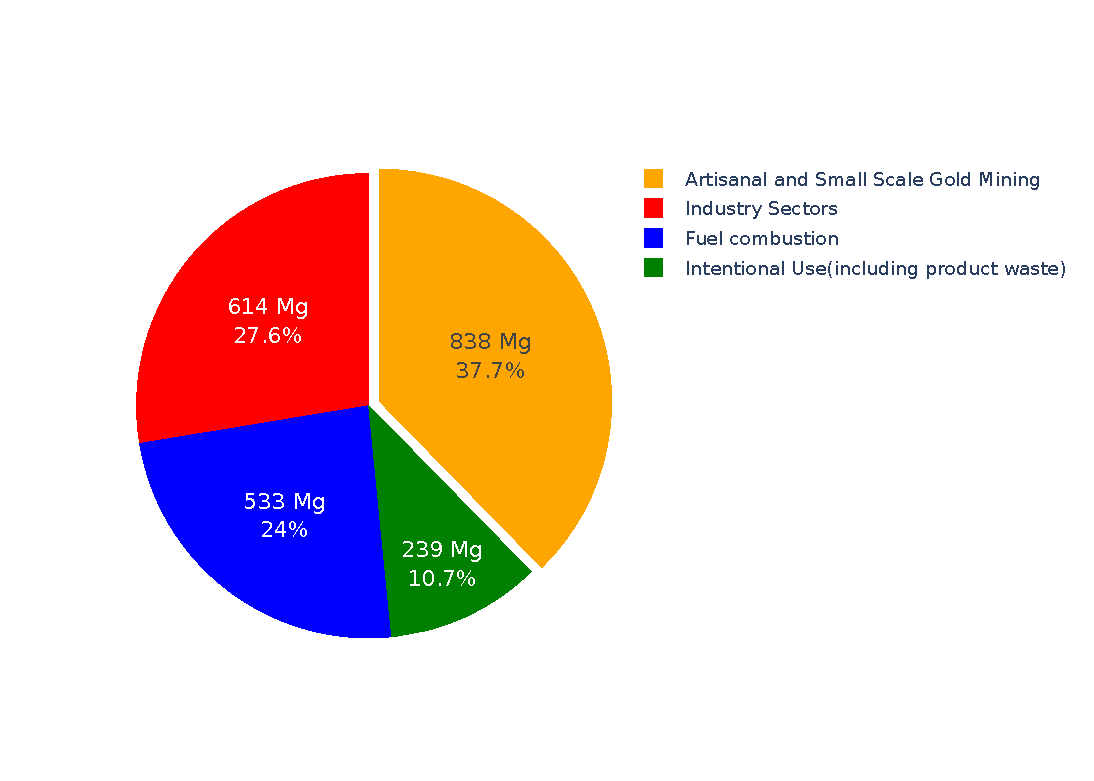
\includegraphics[width=0.8\textwidth]{templates/figures/07-24-22_gma2018_hg-emissions_by-industry.pdf}
  \centering
  \caption{Pie chart showing the 2018 global mercury assessment (GMA 2018) ASGM \hg emission estimates for different sectors. ASGM is the sector with the highest Hg emissions (shown in orange) at 838 Mg, followed by industry sectors (shown in red) at 614 Mg, then fuel combustion (shown in blue) at 533 Mg, and finally, intentional use sectors excluding ASGM (show in green) at 239 Mg \cite{united_nations_environment_programme_technical_2019}.}
  \label{fig:gma2018_hg-emissions_by-industry}
\end{figure}
\FloatBarrier

\section{Motivation}
\begin{flushleft}
While most of the Hg pollution from ASGM is local, its ability to travel across borders and contaminate distant ecosystems bolsters the case for concerted global efforts to eliminate Hg pollution in all forms, including ASGM Hg pollution. The Minamata Convention (MC) is a legally binding global treaty to protect human health and the environment from the adverse effects of mercury. Its text comprises articles that also target ASGM Hg emissions\cite{unep_minamata_2013}. Article 22 of the MC demonstrates the importance of consistent and scientifically rigorous reporting, including reporting from ASGM, about Hg releases and emissions, if sound policies and management actions are to be developed that promote sustainable change. 
\end{flushleft}
\begin{flushleft}
More than 100 million people depend on artisanal and small-scale gold mining (ASGM) for their livelihood globally, particularly in the over 81 countries, predominantly in the global south where ASGM exists\cite{planetgold_planetgold_2021}. Additionally, ASGM is an essential source of income and an opportunity for rural development in countries where options and alternatives to ASGM for generating income to buy necessities of daily life are in short supply or nonexistent \cite{planetgold_planetgold_2021}. It is estimated that around 10 to 20 million (ASGM) miners are employed in the ASGM worldwide - about a third of them are women - and they provide 90\% of the global gold mining workforce and extract about 20\% of the world's gold annually \cite{planetgold_planetgold_2021}. For example, in Peru, ASGM sustains the livelihoods of an estimated 1 million people, and between 300,000 and 500,000 miners were involved in Peru's ASGM sector as of 2014. Despite being a vital source of livelihood for the communities that practice ASGM, its activities often lead to several environmental, human, and social harms. In addition to Hg releases to the environment, ASGM externalities include deforestation, tropical diseases such as malaria, dangerous and unsafe working conditions, crime and exploitation of indigenous communities, diesel and gasoline spills, and human trafficking \cite{usaid_usaid_2020}. 
\end{flushleft}

\section{Artisanal and Small-Scale Gold Mining}

\begin{flushleft} 
During ASGM, Hg is added to the gold ore to form a mercury-gold amalgam, a mixture of about equal amounts of Hg and gold\cite{united_nations_environment_programme_reducing_2012}. Heat is applied to the amalgam, which evaporates the Hg, leaving the gold behind. Gold extraction using this method is popular with the ASGM community since it is inexpensive, easy to use, and quick \cite{united_nations_environment_programme_reducing_2012}. Moreover, Hg is relatively effective at capturing gold when there are no other options but often captures less than 40\% \cite{united_nations_environment_programme_developing_2015}. There is usually a tremendous amount of Hg vapor in the air around amalgam burning sites, much higher than the World Health Organization(WHO) limit of 1.0 $\mu$g/m$^{3}$\cite{gibb_mercury_2014}. The Hg emissions in ASGM are harmful to miners and members of their communities.
Additionally, humans and ecosystems far away are also exposed to Hg risks because Hg travels globally through the atmosphere. As vaporized Hg settles in soil, rivers, bays, and oceans, anaerobic organisms transform it into methylmercury, and water bodies can become contaminated with methylmercury\cite{united_nations_environment_programme_technical_2019}. Methylmercury is absorbed and ingested by phytoplankton, zooplankton, and fish, and predator species such as sharks and swordfish that live a long time accumulate methylmercury and are usually the source of poisoning for people who eat fish\cite{gibb_mercury_2014}. Figure \ref{fig:world_hg_emisions} shows how the annual average of the total Hg emissions from  all global anthropogenic Hg emissions sources is distributed. 
\end{flushleft}

\begin{figure}[H]
  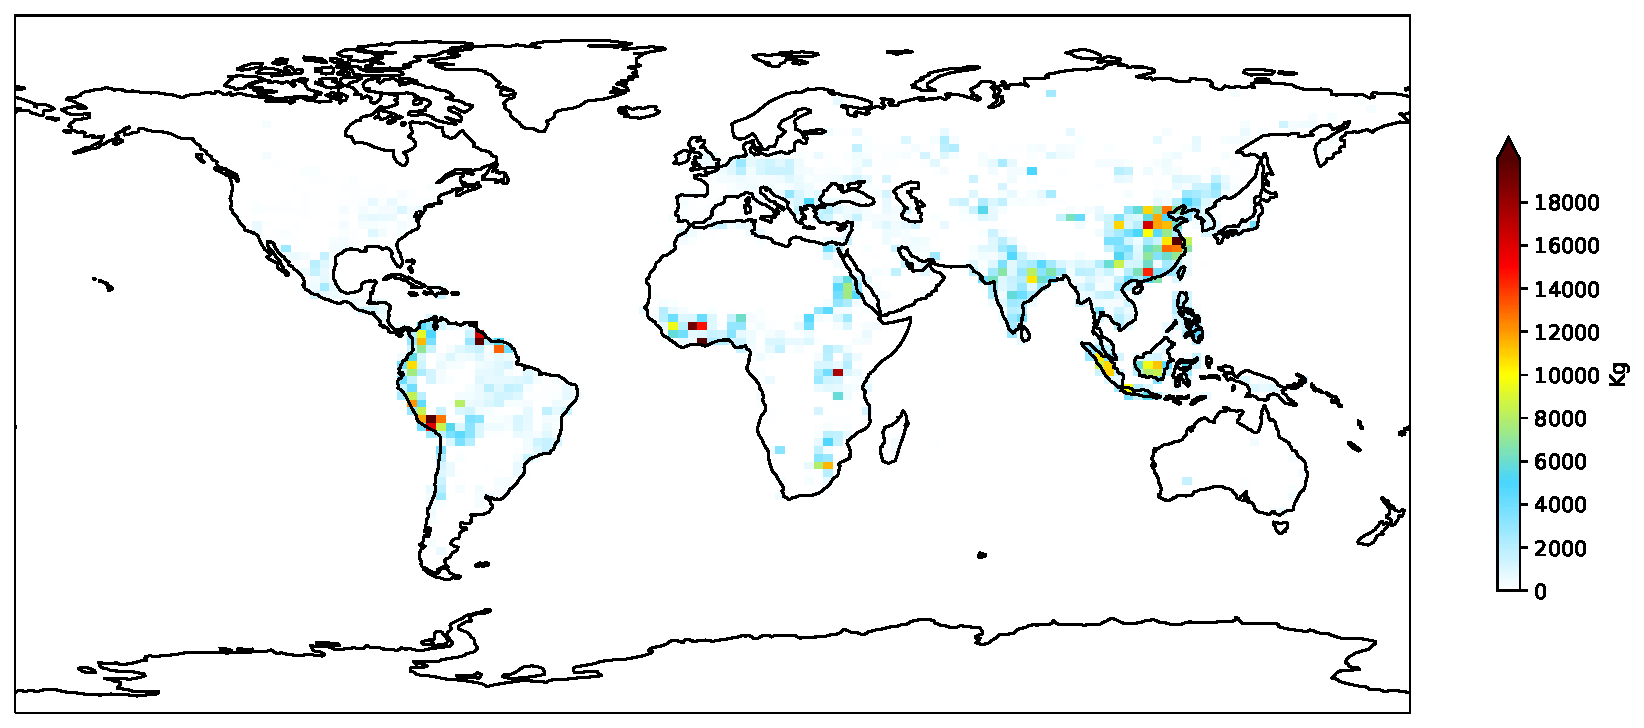
\includegraphics[width=0.8\textwidth]{templates/figures/06-12-22_total_Hg0-emissions-per-year_globally_001.pdf}
  \centering
  \caption{Spatial distribution of annual average Hg anthropogenic emissions for a year between July 2014 and July 2015 \cite{united_nations_environment_programme_technical_2019}}
  \label{fig:world_hg_emisions}
\end{figure}
\FloatBarrier

\section{ASGM Measures in the Minamata Convention}
\begin{flushleft}
    

The MC is a global treaty that was agreed upon at the fifth meeting of the Intergovernmental Negotiating Committee on Hg in Geneva, Switzerland, in January 2013 and formally adopted in October that year in Kumamoto, Japan. Moreover, the treaty entered into force on 16 August 2017, 90 days after the 50\textsuperscript{th} instrument of ratification was deposited, and currently has 137 parties to the convention\cite{unep_minamata_2013}. The MC's goal is to protect human health and the environment from the adverse effects of mercury, and it affirmed that global action is essential to address the Hg pollution problem. Article 7 and Annex C of the MC target ASGM. Article 7 requires countries where Hg is used in ASGM to develop a National Action Plan (NAP) that details ways to reduce and, where possible, eliminate the use of Hg and Hg compounds. Each country should include in its NAP actions to stop some of the worst practices of ASGM, which include, among other things, (i) whole ore amalgamation, (ii) open burning of amalgam, (iii) burning of amalgam in residential areas (iv), and cyanide leaching in sediment or tailings to which Hg has been added without first removing the Hg \cite{united_nations_environment_programme_technical_2019}.
Moreover, countries are required to include in their NAPs baseline estimates the quantities of Hg used in ASGM. The guidance document on developing a national action plan states that the goal should be to produce an estimate that has an accuracy of $\pm$ 30\% and, at worst, $\pm$ 50\%. The authors argue that this is an obtainable level of confidence in the context of effort, time, and financial resources while being good enough to inform the NAP and allow for prioritization of actions \cite{unep_developing_2017}. A vital component of the MC is Article 22, which specifies a variety of information that must be included when conducting the effectiveness evaluation of the MC. The article states that "the Conference of the Parties shall, at its first meeting, initiate the establishment of arrangements for providing itself with comparable monitoring data on the presence and movement of Hg and Hg compounds in the environment as well as trends in levels of Hg and Hg compounds observed in biotic media and vulnerable populations." In addition, the MC secretariat recently published the monitoring guidance, which explains the role of monitoring in the effectiveness evaluation and sets realistic expectations about what can be learned over time, among other guidance goals \cite{unep_guidance_2021}. 
\end{flushleft}

\section{Case Study Region}
\begin{flushleft}
Based on Yoshimura et al.'s (2021) estimate of mercury losses and gold production by ASGM, Latin America has the highest average ratio of mercury losses to gold production, 4.63, while Africa and Asia have the lowest at 1.96 and 1.23, respectively. Moreover, the GMA 2018 reported that ASGM Hg emissions in Latin America were the highest, and Figure \ref{fig:global_asgm_emissions_above_a_tone_barchart} shows that Peru is one of the top emitters of ASGM-related Hg and 60\% of the top 10 ASGM Hg emitting countries in the world are in Latin America  \cite{united_nations_environment_programme_technical_2019}. However, atmospheric Hg data from Latin America are rare; hence Hg dynamics in the region are not well understood. 
\end{flushleft}
\begin{figure}[H]
  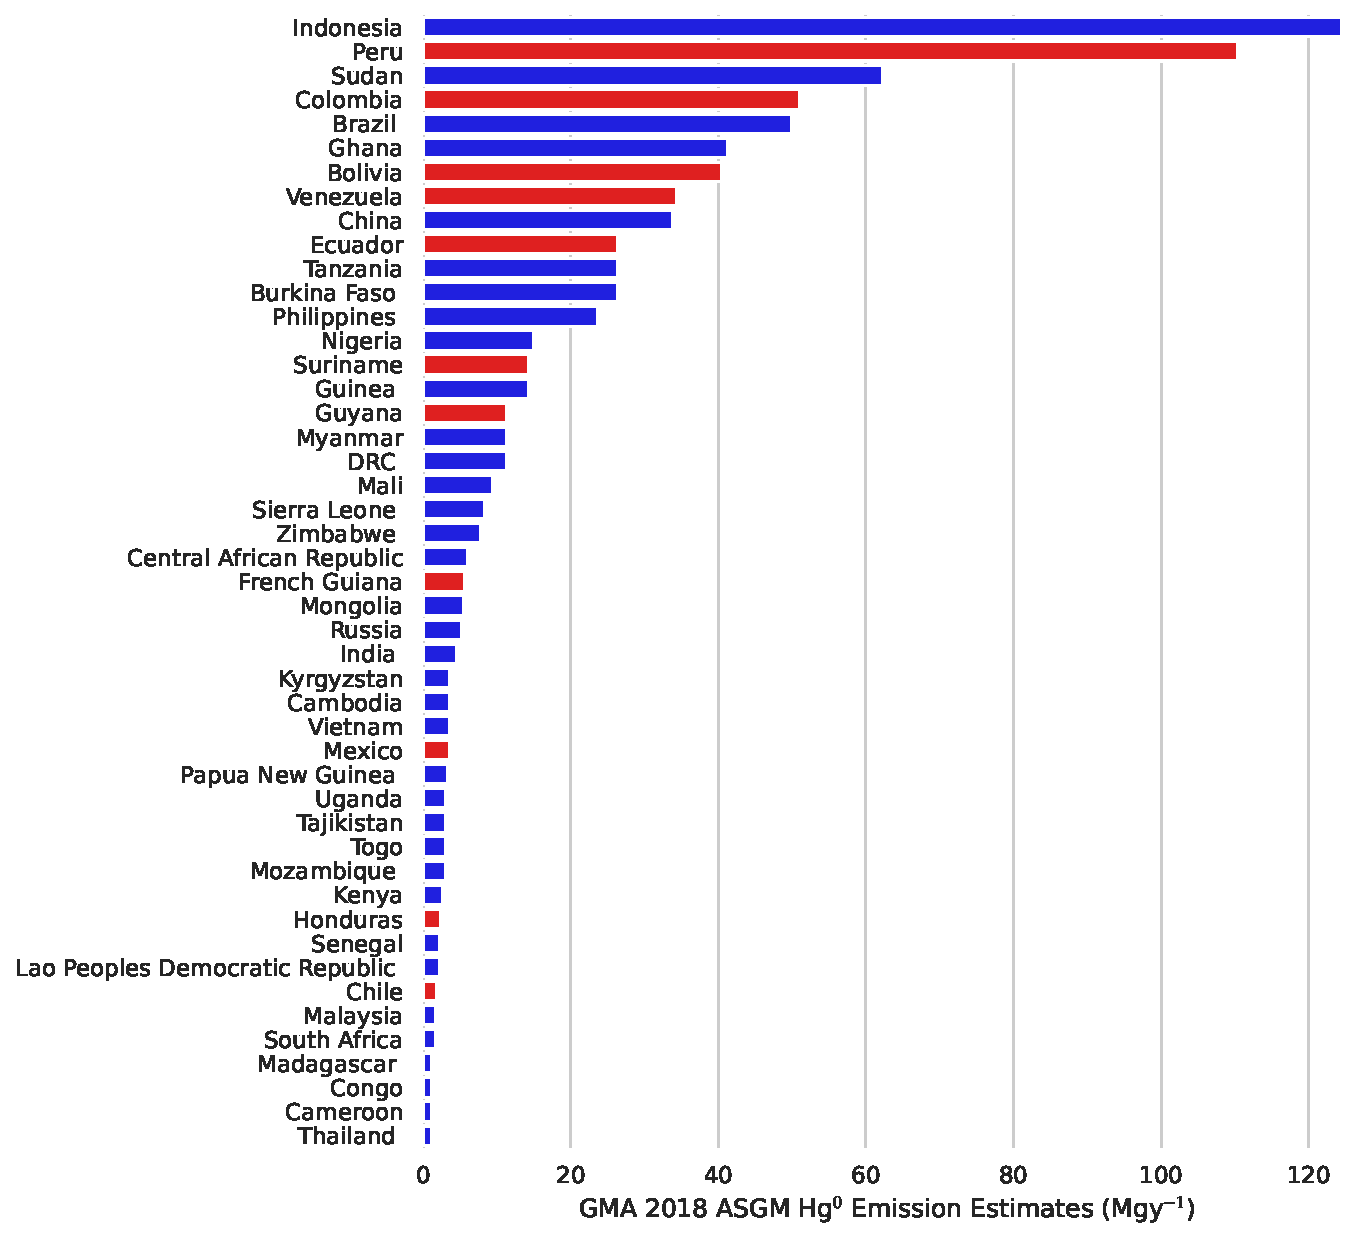
\includegraphics[width=\textwidth]{templates/figures/07-14-22_gma2018_top-asgm-emmiting-countries.pdf}
  \centering
  \caption{Bar chart showing the GMA 2018 ASGM \hg emission estimates for all countries worldwide that have estimated ASGM \hg emissions above 1 Mg. The red bars highlight countries in Latin America \cite{united_nations_environment_programme_technical_2019}}
  \label{fig:global_asgm_emissions_above_a_tone_barchart}
\end{figure}
\FloatBarrier
\begin{flushleft}
Additionally, Peru is the source of the largest ASGM emissions in Latin America, as seen in Figure \ref{fig:global_asgm_emissions_above_a_tone_barchart} and the Madre de Dios region in Peru was estimated to have released the largest quantities of Hg to the environment and the atmosphere\cite{agc_reporte_2017}. Madre de Dios, shown by the red outline in Figure \ref{fig:PeruCS} is a rainforest region between Bolivia and Brazil and covers roughly 85,000 square kilometers. The region's name is derived from the name of a major river that runs through it, and smaller streams and rivers cross through it to provide transportation and fishing for indigenous communities. Furthermore, these waterways are the main sites of ASGM and, subsequently, Hg contamination \cite{ashe_elevated_2012,agc_reporte_2017}. 
\begin{figure}[H]
  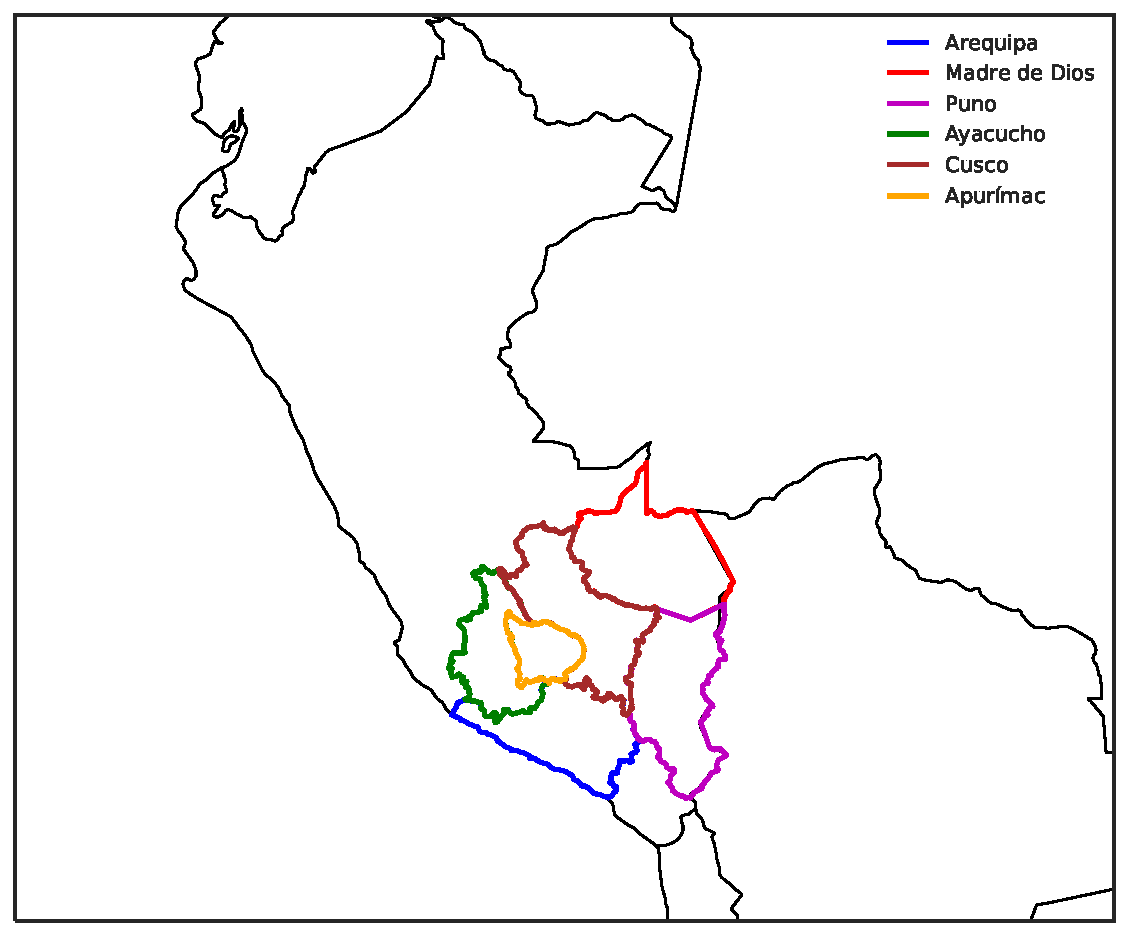
\includegraphics[width=0.6\textwidth]{templates/figures/Peru_Maps/CasestudyRegion.pdf}
  \centering
  \caption{Departments predicted to be the prominent sources of ASGM Hg releases according to the Artisanal Gold Council's  Inventory Report for the ASGM sector in Peru (2017) }
  \label{fig:PeruCS}
\end{figure}
\FloatBarrier

Hg has been extensively studied in Madre de Dios, both in people and in the environment. Therefore, this thesis project seeks to complement previous studies and distinguishes itself  by investigating the extent to which the GEOS-Chem model can leverage existing measurements of Hg in the atmosphere and bottom-up Hg emission estimates in published Hg global and national inventories to constrain the amount of ASGM Hg emissions from the case study region in Peru. 

\end{flushleft}
\begin{flushleft}


\section{Thesis Questions}
According to Evers et al.(2016), country-specific actions under Article 7 of the MC will differ from country to country, and this variability poses a challenge to assessing the MC's effectiveness. Additionally, they argue that changes in the overall use of Hg in the global ASGM sector can be informed by progress in individual countries. They suggest a compilation, visualization, and mapping of the respective data to track this progress across ASGM countries. Moreover, N.E Selin (2014) highlighted that the existing global-scale monitoring networks for background Hg levels could not indicate whether the MC would lead to changes in the global biogeochemical cycling of Hg. She further argued that monitoring policy effectiveness in reducing emissions requires better knowledge of and the ability to explain baseline levels in the global biogeochemical cycle without policy and track potential changes. This value added by baseline estimates of emissions to policy making is also recognized in the MC's paragraph 3 of Article 7, which stipulates that each party that notifies the secretariat that (ASGM) and processing in its territory is more than insignificant shall develop and implement a national action plan (NAP) per annex C to the MC. In addition, annex C (d) states that the NAP shall include baseline estimates of the quantities of Hg used and the practices employed in ASGM and processing. As of this writing, 18 countries have submitted their respective NAPs, and the estimates of how much Hg is used in their territories are shown in Figure\ref{fig:global-hg-emission-estimates_vs_nap_estimates}. 

\begin{figure}[H]
  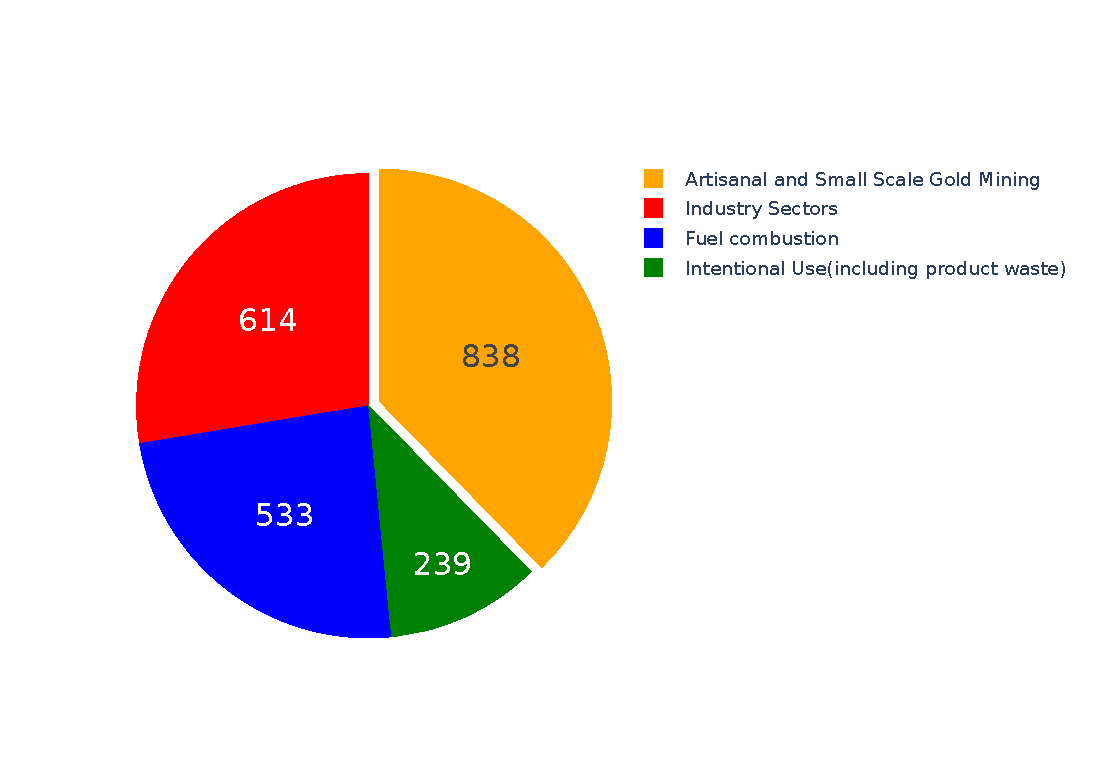
\includegraphics[width=\textwidth]{templates/figures/07-24-22_global-hg-emission-estimates_vs_nap_estimates.pdf}
  \centering
  \caption{Bar chart comparing the estimates of annual average Hg emissions predicted in the GMA 2018 inventory in light blue vs. annual average Hg emissions baseline estimates (shown in dark blue) that were reported by the respective countries in their NAPs \cite{united_nations_environment_programme_technical_2019} }
  \label{fig:global-hg-emission-estimates_vs_nap_estimates}
\end{figure}
\FloatBarrier


 It is evident in Figure \ref{fig:global-hg-emission-estimates_vs_nap_estimates} that the difference between the global estimates and the NAP estimates is vast for some countries. While the baseline estimates of Hg use in ASGM as reported in the NAPs and global inventories are critical, data from monitoring networks combined with atmospheric models provide additional tools to evaluate the changes in Hg in the atmosphere. Several studies have identified atmospheric mercury monitoring as a primary and appropriate method to assess the effectiveness of the MC\cite{sprovieri_atmospheric_2016,evers_evaluating_2016,gustin_measuring_2015,united_nations_environment_programme_technical_2019}. Likewise, the monitoring guidance,\cite{unep_guidance_2021} echoes this by emphasizing the provision of data for the development and improvement of transport and chemistry models as one of the primary objectives of monitoring Hg in the atmosphere. Nevertheless, few studies have demonstrated how models can inform policy on ASGM Hg emissions using monitoring data. Consequently, I aim to answer the following questions based on the assumption that using chemical transport models (CTMs) such as GEOS-Chem can provide a means to synthesize data from national and global Hg inventories and atmospheric monitoring networks to track progress and measure MC's effectiveness.:
\begin{enumerate}
  \item To what extent can regional atmospheric modeling and monitoring help reconcile the differences in the current global estimates of emissions and national emissions?
  \item What regional monitoring networks are essential to improve models' effectiveness in evaluating the MC's effectiveness?
  \item Which policies are essential to catalyzing action towards the expansion of regional monitoring, particularly in the regions where ASGM emissions are the dominant source?
\end{enumerate}
\end{flushleft}




 
\section{Organization}
 
\begin{flushleft}
  This introductory chapter has provided a general background on ASGM concerning Hg emissions and the extent of global efforts to protect people and the environment from the adverse effects of Hg pollution. Chapter 2 addresses the first thesis question by evaluating GEOS-Chem modeled atmospheric Hg concentrations across Latin America with observed Hg concentrations at various regional sites. The strengths and limitations of the GEOS-Chem model are highlighted, and strategies to improve the model's usefulness are discussed. Chapter 3 addresses the second thesis question by presenting a method to produce top-down estimates of ASGM Hg emissions and discussing possible network configurations to monitor ASGM Hg emissions. Finally, chapter 4 presents policy recommendations and conclusions to address the third research question.  
\end{flushleft}



%\section{Organization}
%% This is an example first chapter.  You should put chapter/appendix that you
%% write into a separate file, and add a line \include{yourfilename} to
%% main.tex, where `yourfilename.tex' is the name of the chapter/appendix file.
%% You can process specific files by typing their names in at the 
%% \files=
%% prompt when you run the file main.tex through LaTeX.
%% prompt when you run the file main.tex through LaTeX.
\chapter{Use of a Global Model to Understand Atmospheric Mercury Observations at Monitoring Sites in Latin America }
%% BACKGROUND
\begin{flushleft}
Environmental pollution from Hg can damage ecosystems through its transformation into toxic methylmercury and bio-accumulation in food chains. Further, Hg is highly mobile in the atmosphere, allowing it to travel to faraway places, resulting in worldwide distribution of its elemental form, \hg, which can last for as long as six months in the atmosphere\cite{horowitz_new_2017,shah_improved_2021}. Hg in the atmosphere can be classified as gaseous elemental Hg (GEM), gaseous oxidized Hg (GOM), and particulate-bound Hg (PBM) less than 2.5$\mu$m in diameter \cite{lindberg_synthesis_2007,schroeder_atmospheric_1998,landis_development_2002}. In most cases, Hg emissions occur as gaseous elemental Hg0, which is relatively inert and sparingly soluble in water\cite{horowitz_new_2017}. Since most Hg entering ecosystems comes from the atmosphere, monitoring and modeling atmospheric Hg and Hg deposition enables us to understand its biogeochemical cycle. In addition, a better understanding of Hg's circulation in the environment would enable effective policies to reduce its harmful effects.
\end{flushleft}
\section{Background}
\begin{flushleft}

Hg monitoring networks and atmospheric Hg models are closely interconnected in the literature. For instance, Gustin et al., (2015) analyzed the state of the science of monitoring and modeling Hg in the atmosphere to deal with the challenge of developing links between Hg ambient levels, deposition, and ecosystem contamination. Notably, the mutual dependency between atmospheric modeling and monitoring is presented in the MC's "Guidance on Monitoring Mercury and Mercury Compounds to Support the Effectiveness Evaluation of the Minamata Convention," which states that observations are needed not only to detect and quantify changes, but also to improve and evaluate models of mercury transport, fate, exposure, and impacts\cite{unep_guidance_2021}. Similarly, Sprovieri et al. emphasize the importance of making consistent global Hg measurements to validate regional and global-scale models\cite{sprovieri_atmospheric_2016}.  According to Brasseur and Jacob, (2017), it is crucial to have a large ensemble of observations to evaluate atmospheric Hg modeling outputs, and several studies have published results using different ensembles of Hg monitoring data. For instance, Weiss-Penzias et al,(2015) used the GEOs-Chem model to develop an understanding of speciated atmospheric mercury observations at five high elevation sites(4 in the USA and 1 in Taiwan)\cite{weiss-penzias_use_2015}. Until now, no detailed model comparison has been conducted in some world regions with high anthropogenic Hg emissions, such as Latin America. The lack of high-frequency atmospheric Hg monitoring capacity in these regions may have limited studies comparing observations to models in these regions, as shown in Figure \ref{fig:global-hg-monitoring-networks}, which illustrates the distribution of global Hg monitoring networks published in the GMA 2018. As seen in Figure \ref{fig:global-hg-monitoring-networks}, Latin America, Africa, and South East Asia remain significantly behind Europe and North America regarding access to relevant observation ensembles. 
\end{flushleft}

\begin{figure}[H]
  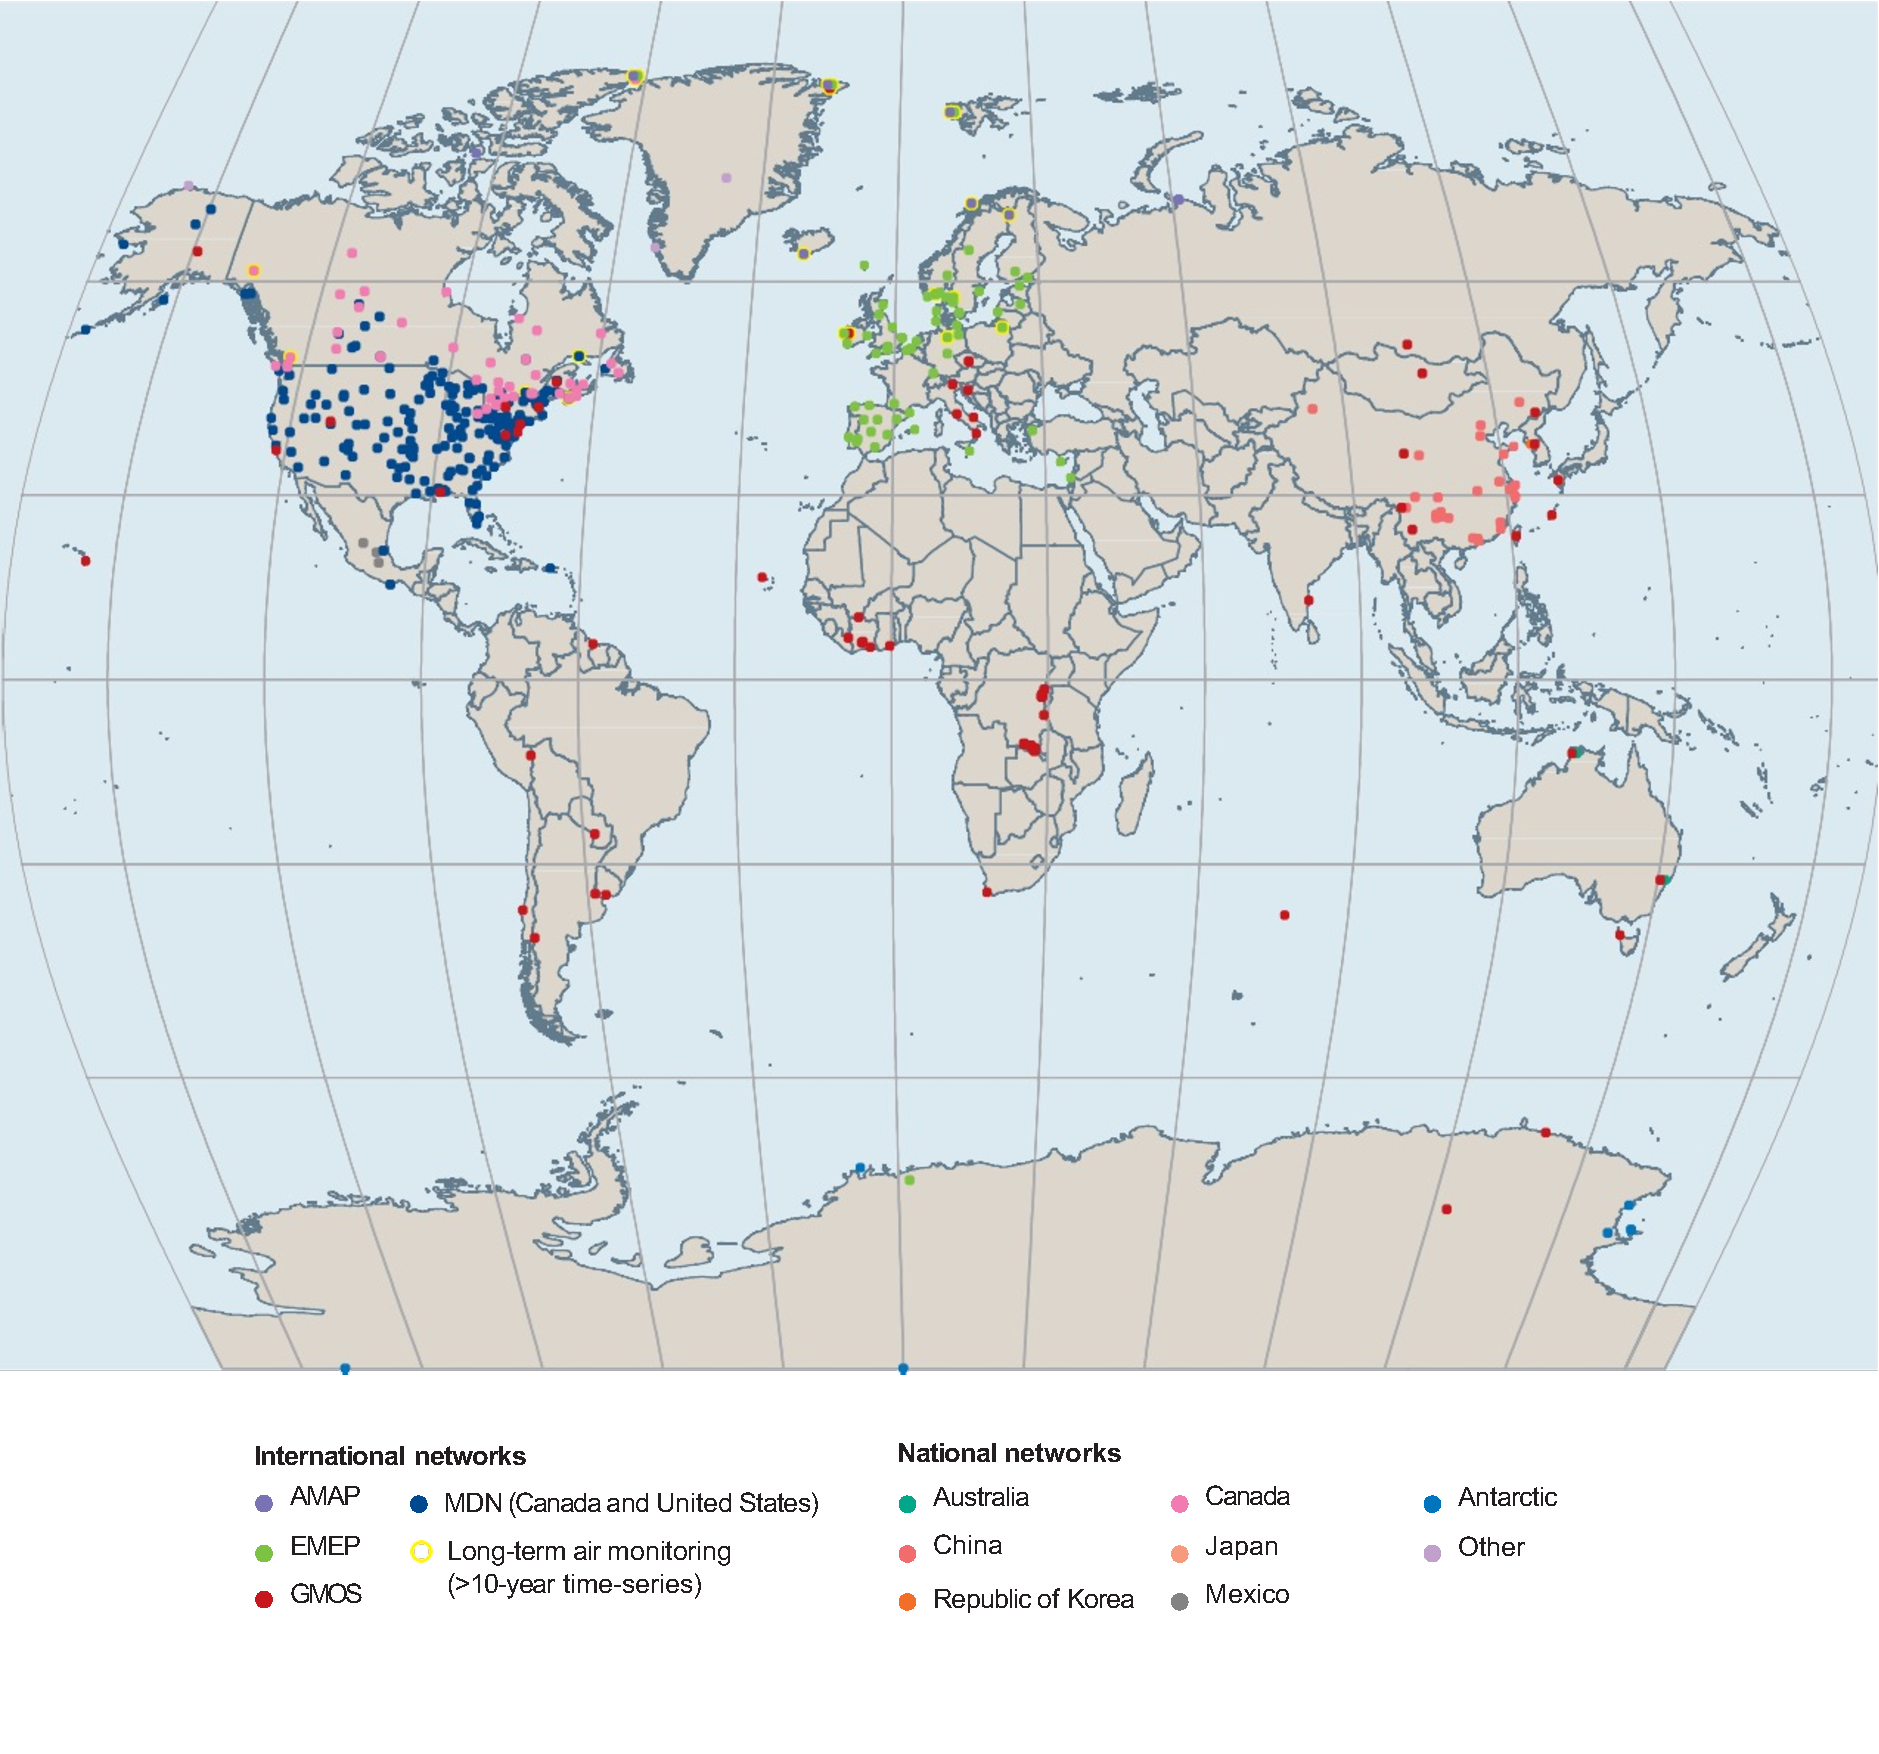
\includegraphics[width=\textwidth]{templates/figures/global-hg-monitoring-networks.pdf}
  \caption{Global map of Hg monitoring networks \cite{united_nations_environment_programme_technical_2019}}
  \label{fig:global-hg-monitoring-networks}
  \centering
  
\end{figure}
\FloatBarrier

\begin{flushleft}
 In this chapter, I compare outputs of the GEOS-Chem model with observed Hg at multiple sites in Latin America. I combine simulations of Hg in the atmosphere produced by the \gc CTM (Sect. 2.2.1) with ground-based observations of atmospheric total gaseous mercury (TGM) (Sect. 2.2.2) from the Global Mercury Observation System (GMOS)\cite{sprovieri_atmospheric_2016} and gaseous elemental mercury (GEM) data from a network of passive air samplers (PAS) distributed across Latin America. Section 2.3 presents results and discussion\cite{quant_measuring_2021}. Comparisons of observations and model outputs are given in Sect. 2.3.1. Finally, I discuss the implications of the current state of atmospheric monitoring and modeling atmospheric Hg in Latin America (Sect. 2.3.2) and summarize my conclusions (Sect. 2.4).
\end{flushleft}




%%----------------------------METHODS-------------------------------------------
\section{Methods}
\subsection{GEOS-Chem Description}
\begin{flushleft}


The global atmospheric Hg concentration was simulated using version 12.8.1 of GEOS-Chem, whose Hg simulation is described by Horowitz et al. (2017)\cite{horowitz_new_2017}. All the simulations in this study were run globally for 47 vertical layers at a resolution of 2.0$\times$2.5, which is approximately equal to a 222 km$\times$277.5 km grid square at the equator \cite{horowitz_new_2017}. Moreover, the MERRA-2 assimilated meteorological data,\cite{gelaro_modern-era_2017} drive the model's atmospheric transport, which calculates atmospheric Hg from three tracers: elemental Hg, Hg\textsuperscript{0}, divalent Hg, Hg\textsuperscript{2+}, and particulate-bound divalent Hg,Hg\textsuperscript{p}. The Hg chemical scheme in the GEOS-Chem version used in this study considers bromine (Br) to be the primary \hg oxidant\cite{horowitz_new_2017} and employs monthly mean Br oxidant concentrations from Schmidt et al.,(2016)\cite{schmidt_modeling_2016}. 
\end{flushleft}
\begin{flushleft}
\subsection{GEOS-Chem Simulations}
The GMA 2018 emissions inventory was used to represent anthropogenic emissions sources from all sectors\cite{steenhuisen_development_2019}. Different inputs to the GEOS-Chem model, such as emissions sources, can be toggled on or off depending on the research objective; hence a reference simulation, \on was created by turning on all Hg emissions sources globally. Moreover, a \off was generated by turning off the ASGM source globally to evaluate the contribution of ASGM to the baseline \hg in the atmosphere by calculating the difference between the \on and \off.
\end{flushleft}


\begin{table}[H]
\captionof{table}{Description of GEOS-Chem Simulations Conducted}
\label{tab:geos_chem_simulation_description}

\centering
\resizebox{\textwidth}{!}{\begin{tabular}{lcp{0.6\linewidth}}

Simulation Name  & Resolution & Description  \\
                        
\hline
Base (ASGM=ON)         & 2.0$\times$2.5 & All Hg anthropogenic emission sources are turned on  \\
No ASGM (ASGM=OFF)        & 2.0$\times$2.5 & All ASGM emissions are turned off

\end{tabular}}

\end{table}
\begin{flushleft}
 The frequency of the simulation output was set to output daily \hg averages at the global scale, while the \hg output for the grid boxes corresponding to the locations of the GMOS observation sites was set to an hourly frequency. The GEOS-Chem outputs for all the simulations conducted were in units of parts per trillion (ppt) and were converted to \nang at standard temperature and pressure (273 K, 1 atm) to compare them to observations.
\end{flushleft}

\subsection{Monitoring Site Characteristics}
\begin{flushleft}
 The GMOS network is one of a few major global projects to develop a global observing system for mercury pollution. GMOS aims to provide high-quality Hg data sets in the Northern and Southern hemispheres to enable a more comprehensive assessment of atmospheric Hg concentrations and their dependence on meteorology, long-range atmospheric transport, and atmospheric emissions\cite{sprovieri_atmospheric_2016}. A vast network of ground-based monitoring stations, regular oceanographic cruises, and lower, upper, and stratospheric measurements make up this European Union-funded project \cite{koenig_seasonal_2021,sprovieri_atmospheric_2016}. More than 40 ground-based monitoring sites constitute the international network, covering many regions with limited to no observational data available before GMOS\cite{sprovieri_atmospheric_2016}. The GMOS monitoring network has five sites in Latin America that actively monitor Hg levels. An analysis of the characteristics of the Sisal, Calhau, Manaus, Nieuw Nickerie, and Bariloche sites has been published by Sproviery et al., (2016), and the Chalcataya site has been analyzed in detail by Koenig et al., (2021) \cite{koenig_seasonal_2021,sprovieri_atmospheric_2016}. A summary of the sites' characteristics is shown in Table \ref{tab:gmos_sites_info}  and they are shown by red triangles in Figure \ref{fig:Latam_Passive_SamplerSites}. A primary objective of this study was to evaluate the degree to which ASGM Hg emissions affected the Hg concentrations in the atmosphere at regional and global scales, so high-frequency GMOS data were collected to facilitate this evaluation.
  \end{flushleft}
  
  \begin{table}[H]
\captionof{table}{The GMOS Sites Evaluated \cite{koenig_seasonal_2021,sprovieri_atmospheric_2016}. }
\label{tab:gmos_sites_info}

\centering
\resizebox{\textwidth}{!}{\begin{tabular}{llccp{0.2\linewidth}rcll}
  \hline

Site                        & Site      & Latitude  & Longitude & Physical  & Elevation    & Number of      & Site &  Measurement  \\
                            & abbrev    &           &           &  Setting  & (m)           & Records (days) & Type&   Period \\
\hline
Sisal, Mexico               & SIS       & 21.16     & -90.05    &   Coastal site        &   7           &   320 &   Secondary    & 1/1/2010-1/1/2016   \\
Calhau, Cape Verde          & CAL       & 16.86     & -24.87    &   Coastal site        &   10          &   309 &   Secondary   & 1/1/2013-12/1/2014  \\
Nieuw Nickerie, Suriname    & NIK       & 5.93      & -56.98    &   Coastal site        &   1           &   215 &    Secondary   & 3/1/2007-12/1/2014 \\
Manaus, Brazil              & MAN       & -2.89     & -59.96    &    Amazon site       &  110          &   100 &   Master   & 1/1/2013-12/1/2014 \\
Chalcataya, Bolivia         & CHC       & -16.2     & -68.12    &    Mountain site       &  5340         &   333 &    Secondary   & 7/1/2014-2/1/2016  \\
Bariloche, Agentina         & BAR       & -41.13    & -72.42    &    Mountain site       &  800          &   333 &  Master     & 10/1/2012-7/1/2017 \\
  \hline
\end{tabular}}

\end{table}

  
 \begin{flushleft}
  The GMOS sites are classified as either secondary or master sites in Table\ref{tab:gmos_sites_info} to indicate the type of data collected and the type of equipment used at the site. The secondary sites used the Tekran continuous mercury vapor analyzer, model 2537A/B (Tekran Instruments Corp., Toronto, Ontario, Canada), except for the Nieuw Nickerie site (NIK), Suriname, which used a Lumex RA-915+ mercury analyzer. The master sites used the Tekran model 2537A/B mercury vapor analyzer coupled with their speciation system model 1130 for GOM and model 1135 for particulate boundaries mercury (PBM2.5) with fractions less than 2.5 $\mu$m in diameter to prevent large particles from depositing on the KCl-coated denuder \cite{koenig_seasonal_2021,sprovieri_atmospheric_2016,gustin_measuring_2015}
     
 
\end{flushleft}

\begin{figure}[H]
 \centering
  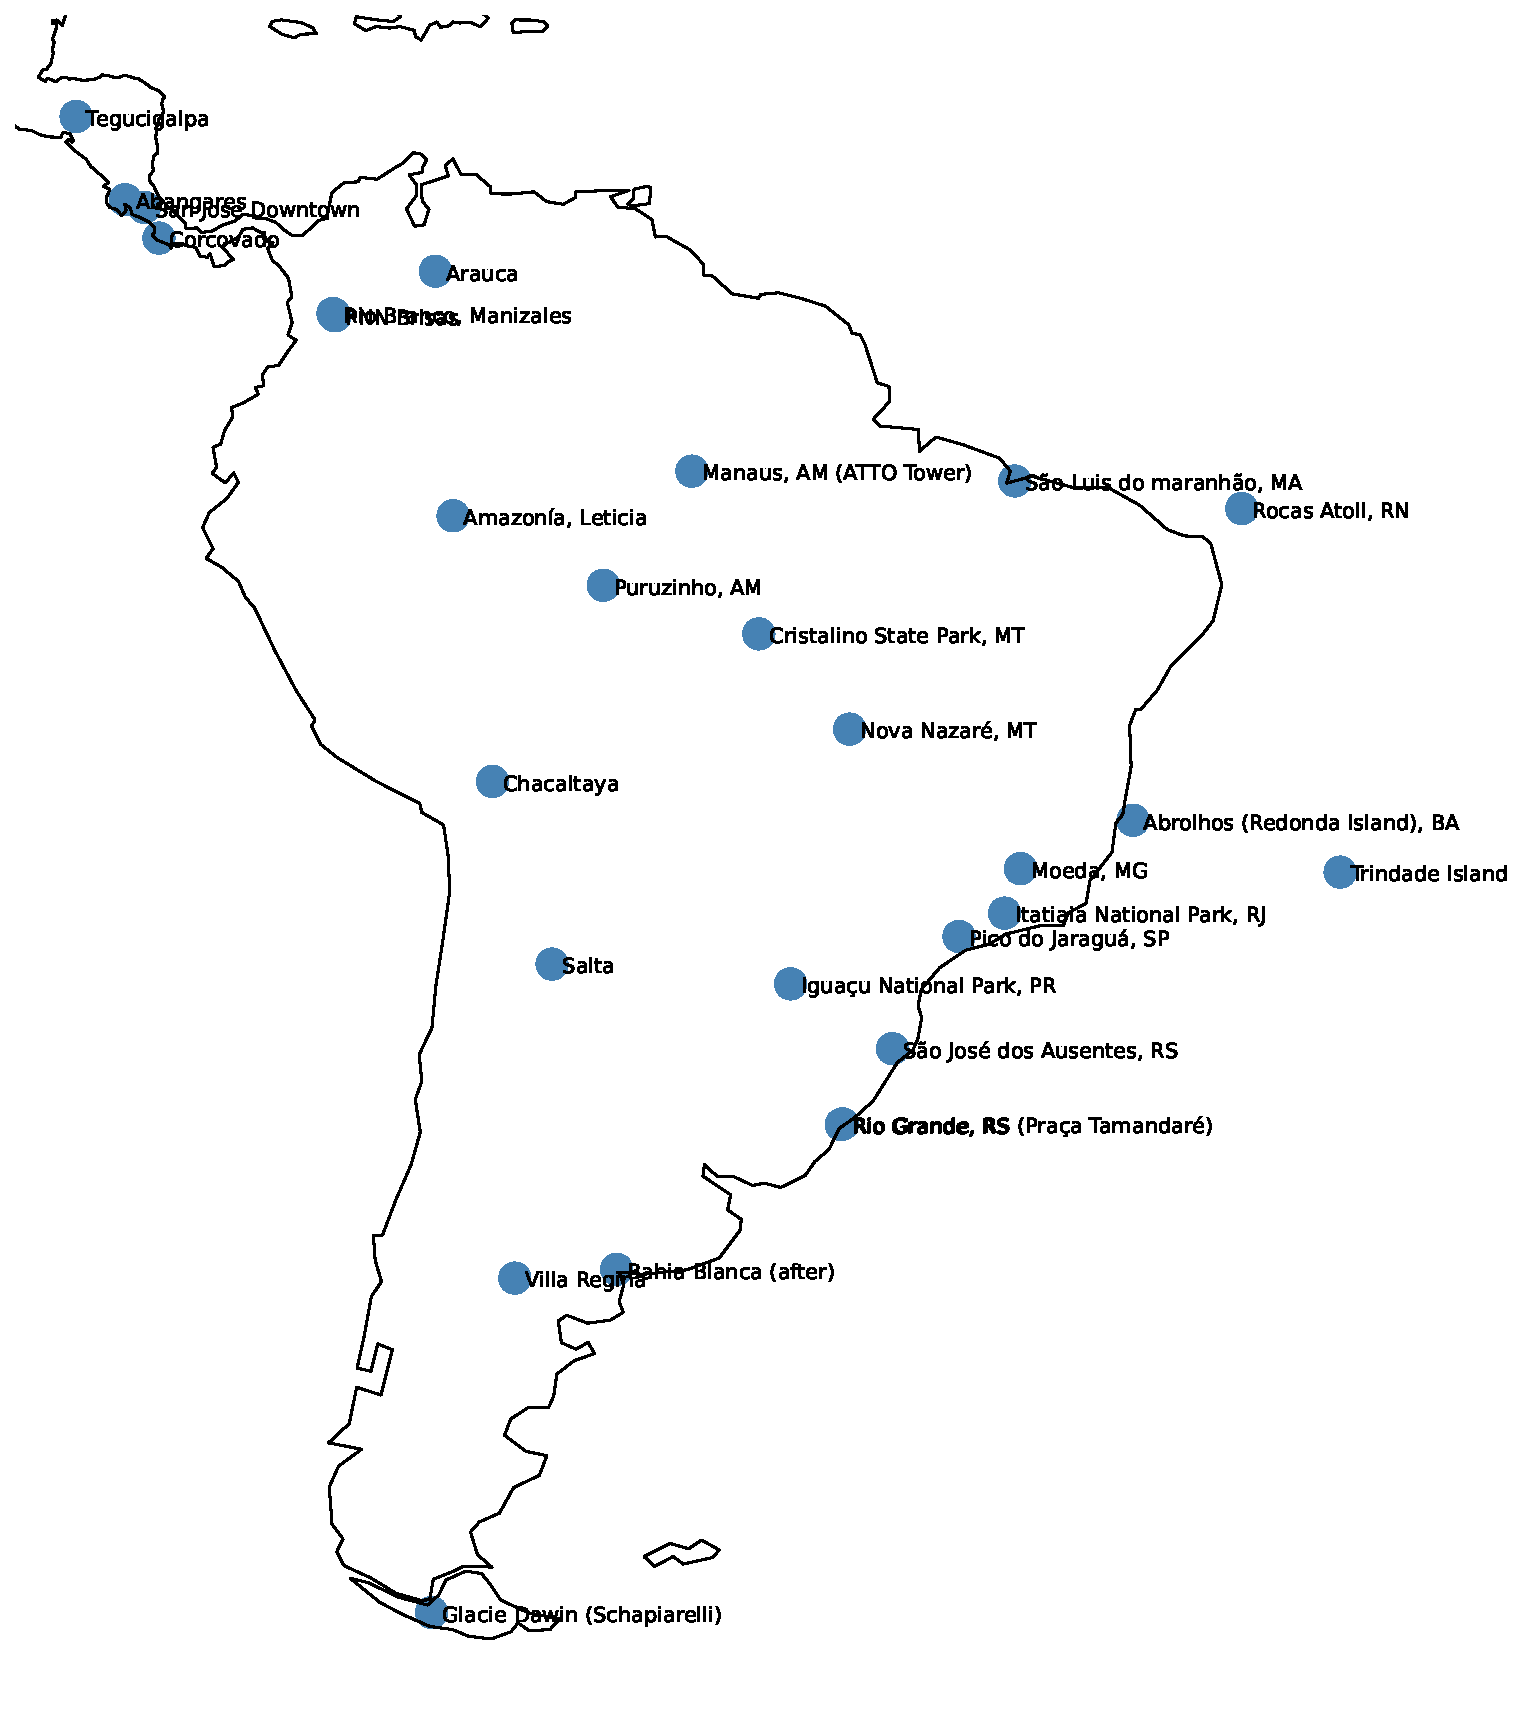
\includegraphics[width=0.8\textwidth]{templates/figures/Passive_Samplers/Latam_Passive_SamplerSites.pdf}
  \caption{Map Showing the GMOS Monitoring Network Sites and Passive Sampler Locations in South America \cite{quant_measuring_2021,koenig_seasonal_2021}}
  \label{fig:Latam_Passive_SamplerSites}
\end{figure}
\FloatBarrier

\begin{flushleft}
    In contrast to active Hg monitoring equipment such as those used in the GMOS network, which can be prohibitively expensive, energy-intensive, and require extensive training, passive air samplers (PAS) require no energy to operate and do not require any special handling skills \cite{quant_measuring_2021}. Furthermore, PAS can be easily deployed for long periods. This combination of attributes of PAS allows more sampling sites to be studied over extended periods enabling significant average GEM concentration estimates to be obtained. PAS monitoring is integral in informing the effectiveness evaluation of the MC\cite{gustin_measuring_2015,unep_guidance_2021}. Quant et al.,(2021) published a detailed analysis of the PAS sites in Latin America, and their respective locations are shown by the blue circles in Figure \ref{fig:Latam_Passive_SamplerSites}. 
\end{flushleft}

\subsection{Observation Data Sourcing and Manipulation}
\begin{flushleft}
  Additionally, average annual GEM concentration data for 27 sites in Latin America was obtained from Quant et al.,(2021), which included information about the coordinates of the deployment sites and the period of measurement \cite{quant_measuring_2021}. Available Hg observation data from the GMOS stations on Figure  \ref{fig:Latam_Passive_SamplerSites} was obtained from the GMOS online database (http://www.gmos.eu), as well as published studies about the Hg monitoring data from the different sites  \cite{koenig_seasonal_2021}. The data sets were pre-processed based on the information in Sproviery et al.,(2016) and Koenig et al.,(2021) and daily and annual averages to compare with the \gc output\cite{koenig_seasonal_2021,sprovieri_atmospheric_2016}. The PAS data was compared to the modeled annual average Hg concentration for 2015 to evaluate, and the coordinate information from the PAS data was used to directly compare the GEM observations and model outputs at the respective PAS sites.
\end{flushleft}





%%----------------------------RESULTS AND DISCUSSION---------------------------
\section{Results and Discussion}

\begin{figure}[H]
\centering
  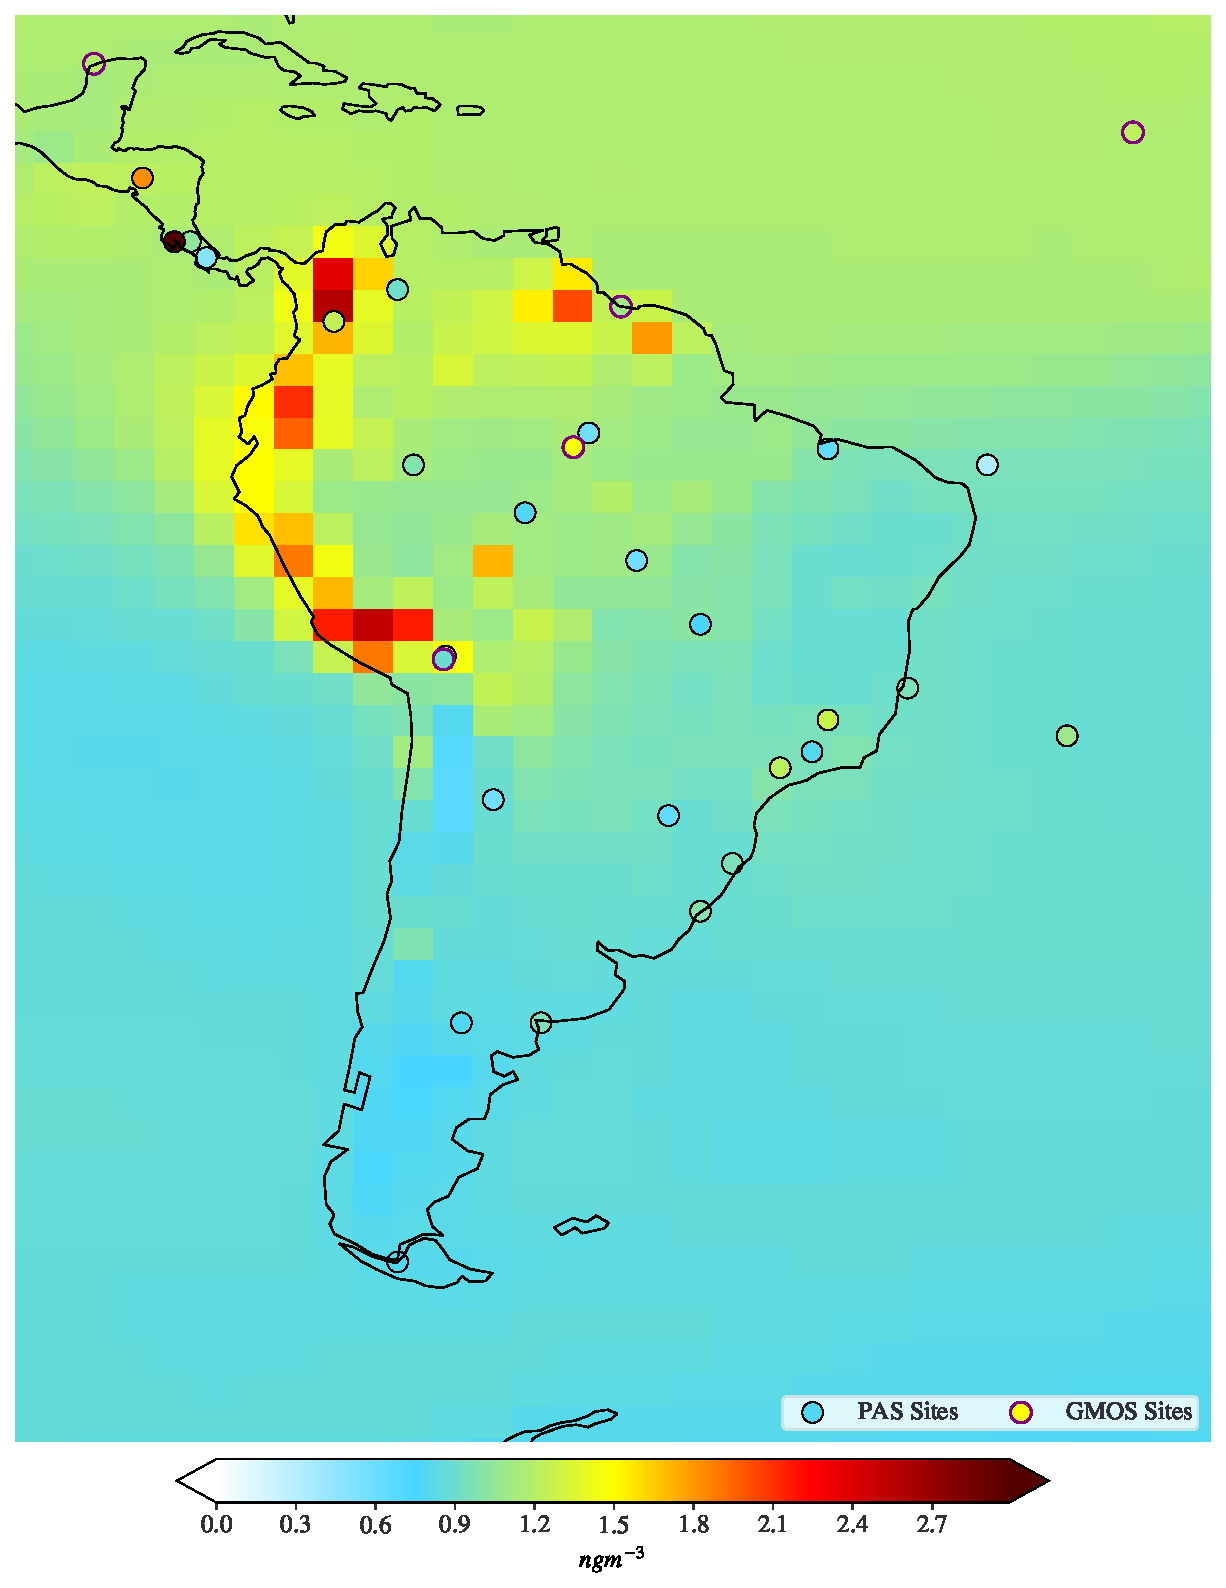
\includegraphics[width=0.7\textwidth]{templates/figures/Passive_Samplers/07-27-22_pas_vs_model_Hg0-per-year_001.pdf}
  \caption{Annual average Hg concentration on the surface in Latin America averaged. The background is the annual average \hgc produced by the \on for 2015. The circles are the annual average GEM concentration from the PAS sites, while the triangles are the annual average TGM concentrations from the GMOS sites.\cite{quant_measuring_2021,sprovieri_atmospheric_2016,koenig_seasonal_2021}}
  \label{fig:06-12-22_pas_vs_model_Hg0-per-year_001}
  
  
\end{figure}
\FloatBarrier
\begin{flushleft}
 Recent publications analyzing global Hg monitoring data highlight an observed interhemispheric gradient of Hg where Hg concentration in the southern hemisphere is lower than Hg concentration in the northern hemisphere\cite{sprovieri_atmospheric_2016}. This gradient is evident in the simulated background annual average \hg concentration as seen in Figure \ref{fig:06-12-22_pas_vs_model_Hg0-per-year_001}. Moreover, most of the GMOS sites validate the modeled interhemispheric gradient except the Chalcataya GMOS site. The model matches the PAS GEM measurement at Chalcataya. This may be explained by the fact that the GMOS Chalcataya Site is a high-altitude site where the Hg concentration was measured at 5340 m above sea level, yet the modeled background shown in Figure \ref{fig:06-12-22_pas_vs_model_Hg0-per-year_001} is the Hg annual average on the surface. Compared with PAS data, the GEOS-Chem model overestimates atmospheric concentrations. Inland sites exhibit this phenomenon more than those located along the coast. There is a difference between the model and the inland PAS sites, especially those in the Amazon region because this version of the GEOS Chem model underestimates Hg uptake by vegetation. Figure \ref{fig:06-12-22_pas_vs_model_Hg0-per-year_by-latitude_001} which shows the modeled (blue circles) and observed (red circles) annual average \hg plotted as a function of latitude clearly indicates the interhemispheric gradient observed in GEOS-Chem. The observation error bars represent the replicate precision of the observations, while the model error bars represent the 95\textsuperscript{th} bootstrap confidence interval for the mean annual \hg. As opposed to the GMOS sites, where GEOS-Chem overestimates the concentrations at all sites, GEOS-Chem only overestimates the concentrations at 15 of the PAS sites, and four of these sites are within the error bars. Evident on Figure \ref{fig:06-12-22_pas_vs_model_Hg0-per-year_by-latitude_001}  is that \gc underestimates Hg concentrations at low latitudes and overestimates those at high latitudes. However, this trend is addressed by the vegetation uptake argument since the Amazon forest is in the northern latitude of Latin America.
\end{flushleft}

\begin{figure}[H]
  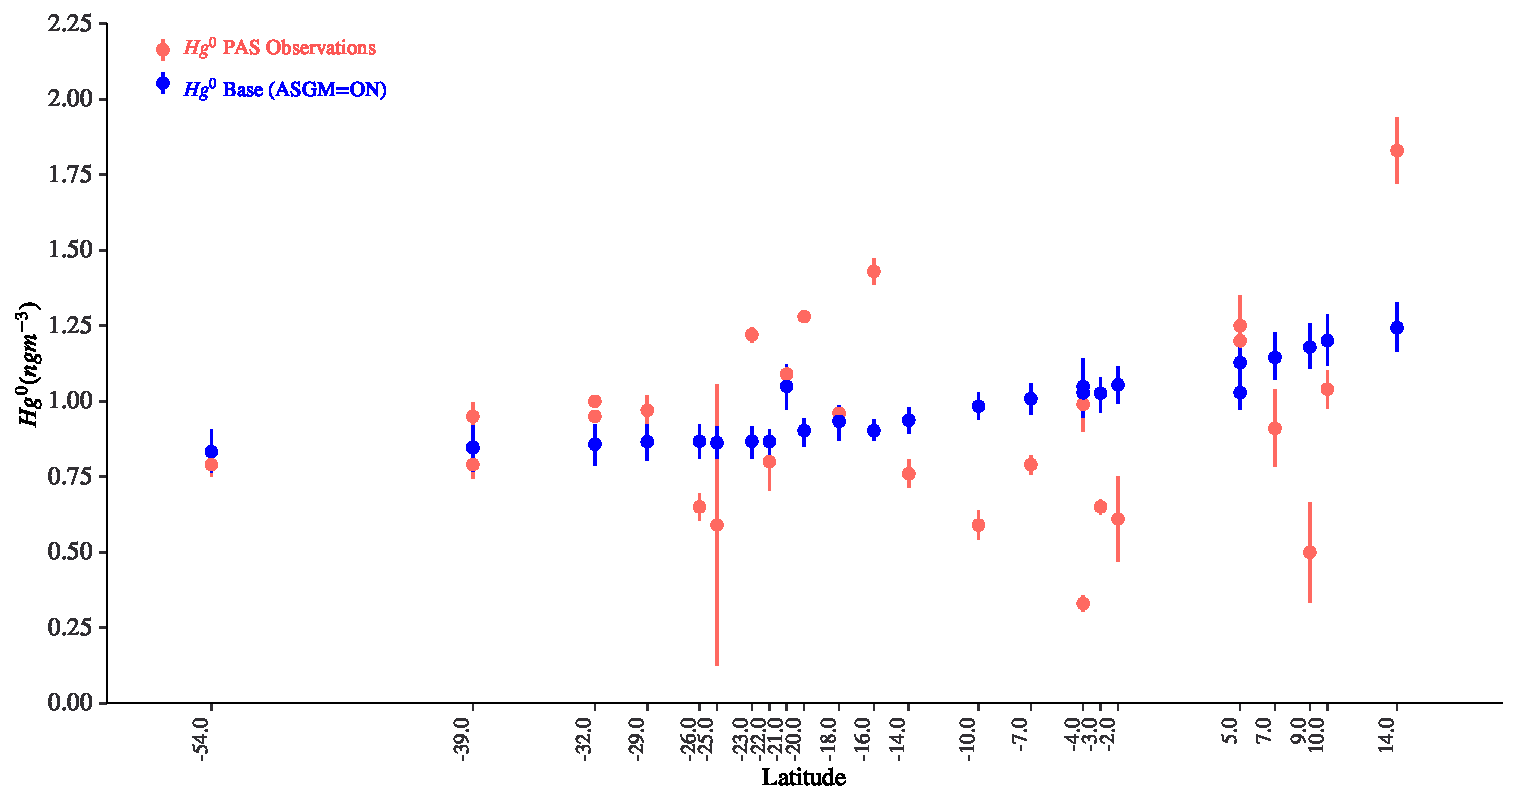
\includegraphics[width=\textwidth]{templates/figures/Passive_Samplers/06-12-22_pas_vs_model_Hg0-per-year_by-latitude_001.pdf}
  \caption{\hg in the atmosphere as a function of Latitude. The \on (blue circles) and observed (red circles) annual average \hg plotted are plotted as a function of latitude to evaluate spatial trends across the continent. The observation error bars represent the replicate precision of the observations while the model error bars represent the 95\textsuperscript{th} bootstrap confidence interval for the mean annual \hg.}
  \label{fig:06-12-22_pas_vs_model_Hg0-per-year_by-latitude_001}
  \centering
  
\end{figure}
\FloatBarrier
\begin{flushleft}
    \gcs overestimation of Hg concentration in the Amazon region observed above was also addressed in Feinberg et al. (2022), who compared simulations with litterfall, throughfall, and flux tower measurements from 93 forested sites to evaluate vegetation as a Hg sink. According to their results, the \gc version, 12.8 underestimates \hg dry deposition, which may explain why measurements of Hg concentration in Latin America were lower than predicted by \gc. 

\end{flushleft}

\subsection{Modeled vs. Observed Temporal Trends}
\begin{figure}[H]
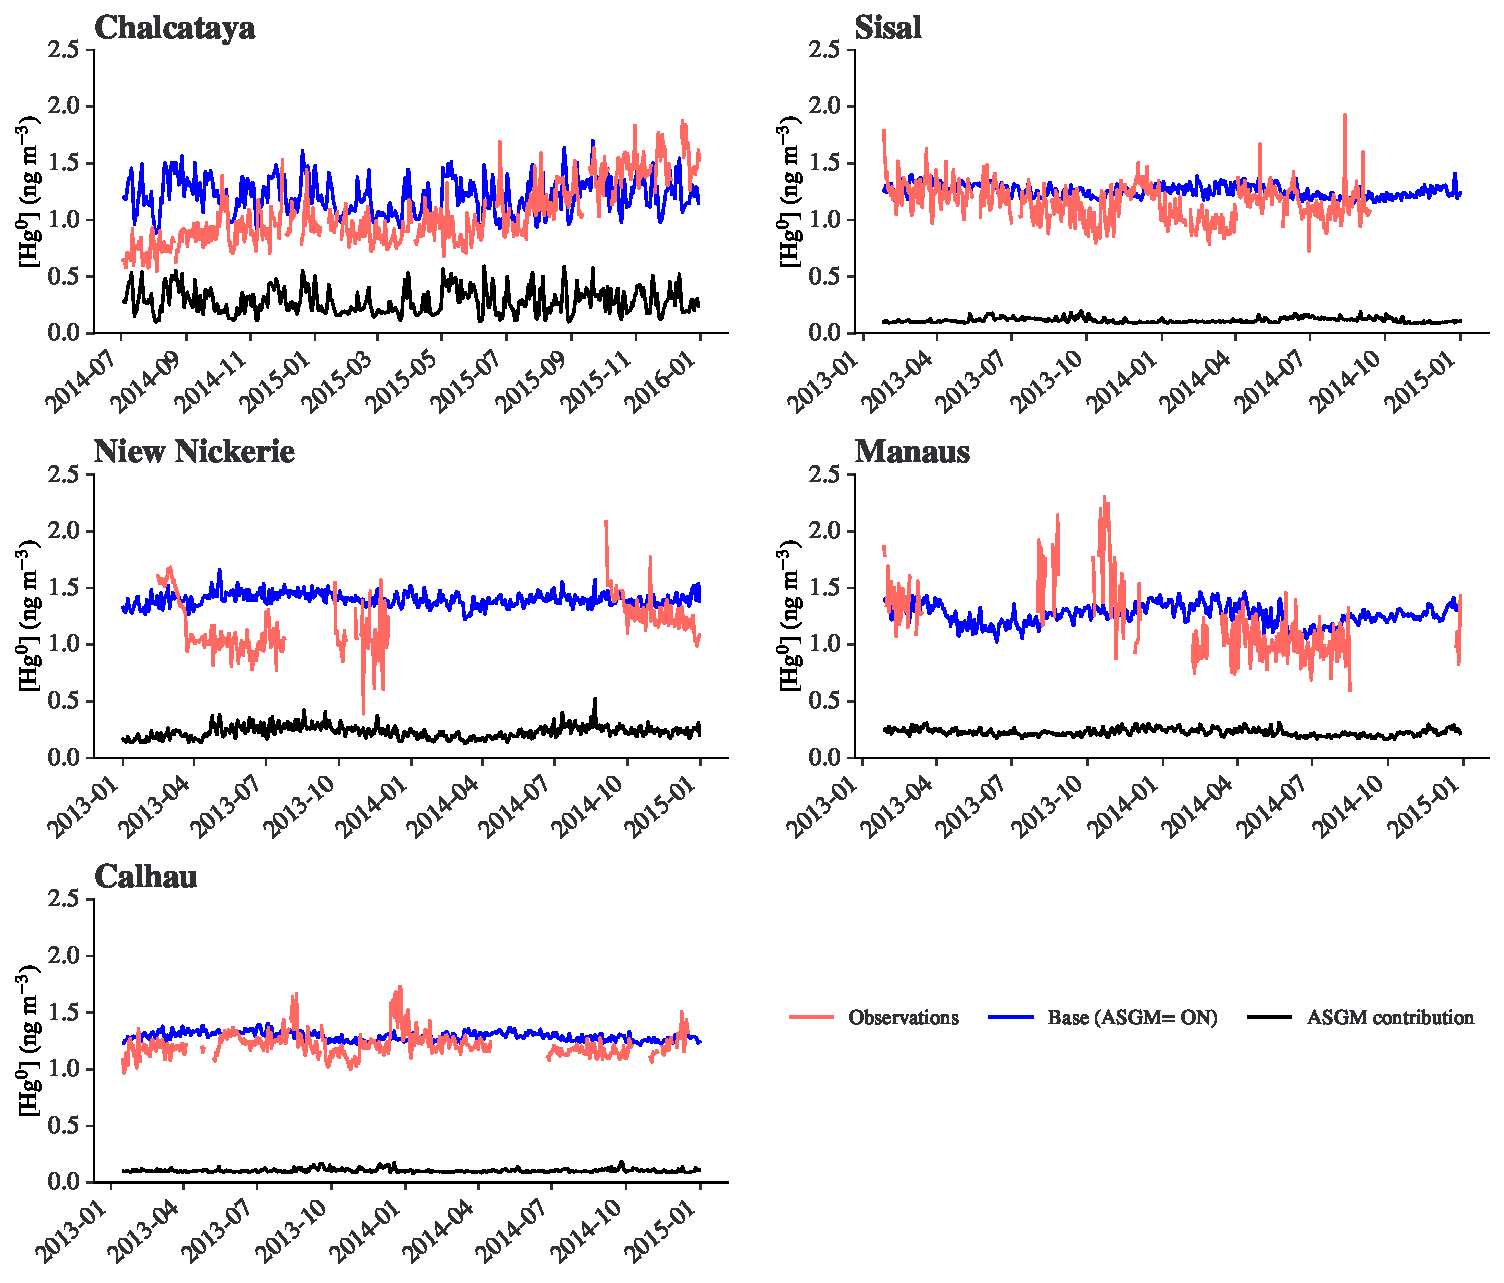
\includegraphics[width=\textwidth]{templates/figures/GMOS_Sites/GMOS_Sites.pdf}
\centering
\captionof{figure}{Time series plots of the observed TGM concentrations at different GMOS sites in red with the corresponding modeled concentration in blue and the associated ASGM contribution in green. Except for the CHC site, where the data are from July 2014 and January 2016, the available data and corresponding model outputs were plotted between January 2013 and January 2016.}
\label{fig:GMOSvsGC}
\end{figure}
\FloatBarrier


\begin{flushleft}


 This study also compared observed and modeled data on a daily resolution as seen in Figure \ref{fig:GMOSvsGC}, which shows the time series of the modeled \hgc in the atmosphere alongside the observed Hg and the simulated ASGM contribution to the atmospheric Hg concentration at the GMOS sites. The \gc model version used in this study overestimated the concentration of Hg on most days. However, the \gc estimated average \hgc over the available observation period was within one standard deviation of the observed Hg in most of the sites except for the Manaus and Nieuw Nickerie sites. \gcs overestimates the observed GEM concentrations at the Manaus and Bariloche master sites by over 25\%  and the GEM concentration at Nieuw Nickerie by 20\%, which may be indicative of poor parameterization of GEM in the model. Moreover, the overestimation of GEM concentrations in Manaus further indicates the model's poor implementation of Hg plant uptake through dry deposition, as discussed in Feinberg et al.(2022)\cite{feinberg_evaluating_2022}.
\end{flushleft}


\begin{figure}[H]
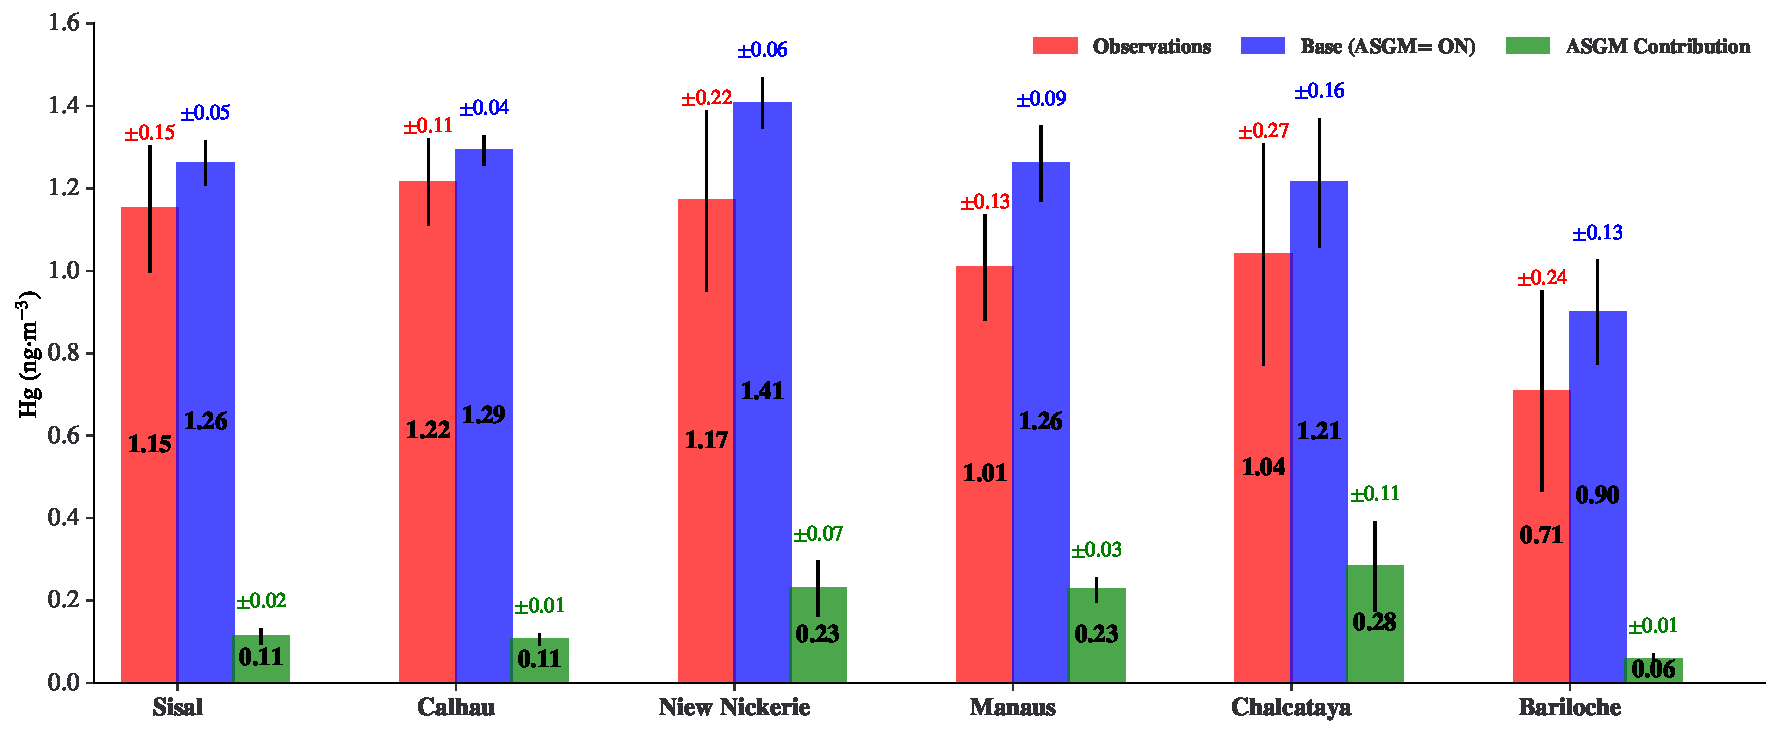
\includegraphics[width=\textwidth]{templates/figures/GMOS_Sites/gmos_sites_stats.pdf}
\centering
\captionof{figure}{Bar chart comparing the modeled and observed average Hg concentration at the respective GMOS Sites. The bars are annotated with the average Hg concentration values. Moreover, the error bars and the annotated value above the bars show the standard deviation in each data set. }
\label{fig:gmos_sites_stats}
\end{figure}
\FloatBarrier
\begin{flushleft}
Moreover, Figure \ref{fig:GMOSvsGC} and Figure \ref{fig:gmos_sites_stats} clearly show that ASGMs modeled contribution is low in most sites except for Calcataya, Manaus, and Nieuw Nickerie. The model's behavior regarding the predicted ASGM contribution at these sites is not surprising since these sites are in countries estimated to be among the top 10 Latin American ASGM Hg emitters in the ASGM emission inventory used for \gc simulation. Even though the model estimates a notable ASGM contribution at the Manaus (18\%) and Nieuw Nickerie (16\%) sites, the sites lack enough data to fully characterize the ASGM contribution to the Hg concentration over the long term. However, the predicted  ASGM Hg contribution at Chalcataya is the highest at 23\% as seen in Table \ref{tab:model_percentage_overestimation_of_mean}. 
\end{flushleft}

\begin{table}[H]
\captionof{table}{Table showing the extent to which the model predicts the observations showed by the percentage difference between the model predictions and the observations }
\label{tab:model_percentage_overestimation_of_mean}

\center
\resizebox{\textwidth}{!}{\begin{tabular}{lcccc}
  \hline

GMOS Site       & Observed Average TGM/GEM  & Modeled Average \hg        &  Percentage difference between       &   Percentage ASGM\\
                &  Concentration (\nang )   &  Concentration (\nang)     &  modeled and observed average (\%)   &   Contribution (\%) \\
                        
\hline
Sisal          &     1.15               &             1.26               & 10                                   & 9 \\
Calhau         &     1.22               &             1.29               & 6                                    & 9 \\
Nieuw Nickerie &     1.17               &             1.41               & 20                                   & 16\\
Manaus         &     1.01               &             1.26               & 25                                   & 18 \\
Chalcataya     &     1.04               &             1.21               & 17                                   & 23 \\
Bariloche      &     0.71               &             0.9                & 27                                   & 6 \\
  \hline
\end{tabular}}
\end{table}


\begin{flushleft}
 Correlations across the time series in Fig.\ref{fig:GMOSvsGC} between observations and the model are shown in Fig. \ref{fig:gmos_sites_scatter}. The general observation is that model poorly matched the observations (mild and even flat slope)  and shallow $r^2$ values. The low correlations between the model and observations may be attributed to poor vegetation uptake, which has already been discussed\cite{feinberg_evaluating_2022}. Moreover, the poor parameterizations of emissions in the model may reduce the extent to which the model recreates the observed atmospheric Hg concentrations. 
\end{flushleft}
 \begin{figure}[H]
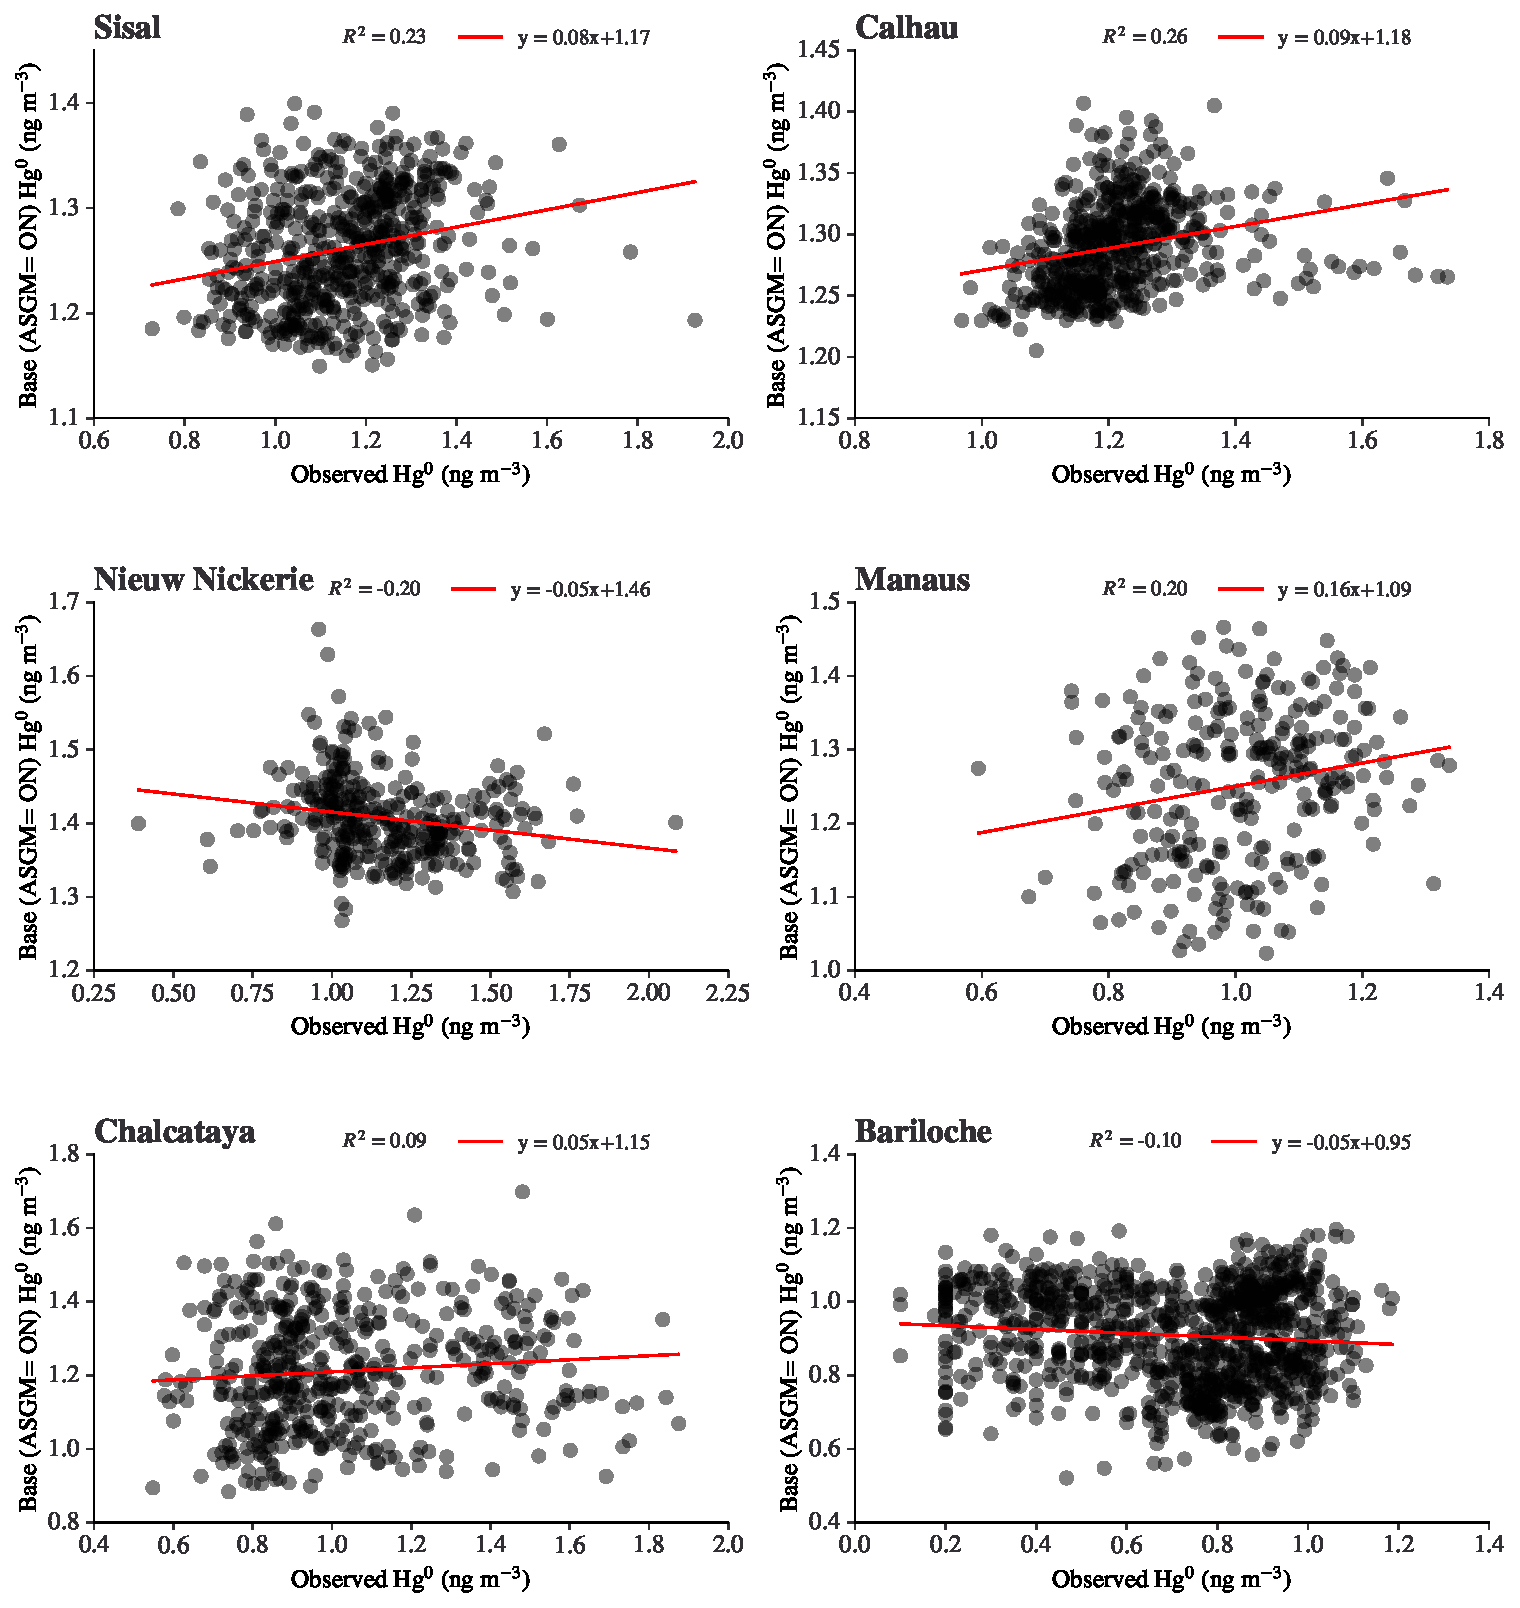
\includegraphics[width=\textwidth]{templates/figures/GMOS_Sites/gmos_sites_scatter.pdf}
\centering
\captionof{figure}{Scatter plots of the modeled Hg concentration as a function of the observed concentration. The red line is used to investigate the extent of the linear relationship between the modeled and observed Hg concentrations}
\label{fig:gmos_sites_scatter}
\end{figure}
\FloatBarrier


\section{Conclusion}

\begin{flushleft}
For this study, we compiled the atmospheric Hg measurements from six GMOS sites across Latin America discussed in \cite{koenig_seasonal_2021,sprovieri_atmospheric_2016}. Additionally, we gathered annual average GEM measurements from 27 PAS sites across Latin America, published in Quant et al.,(2021). These data on the measured atmospheric GEM and TGM concentration in Latin America were compared with \hgc simulated by the GEOS-Chem global Hg model with the oxidation scheme explained in Horowitz et al.,(2017) to examine spatiotemporal trends and test for evidence of ASGM contributions to measured Hg. A relatively weak relationship was found between the observed mercury species (GEM and TGM) and those in the /on, demonstrating a need for an improved understanding of fundamental chemistry in the \gc model.

\end{flushleft}
\chapter{Top-down Constraints on Atmospheric Mercury Emissions from ASGM Activities}
\section{Background}
\begin{flushleft}


 Numerous prior studies have quantified anthropogenic Hg sources, including ASGM Hg emissions using different methodologies. Bottom-up estimates leverage collected data on underlying activities and emission factors to estimate regional and global totals. For instance, the bottom-up global inventory in the GMA 2018 estimated ASGM Hg emissions to be 838 Mg with an uncertainty range of 675-1000 Mg for 2015 \cite{united_nations_environment_programme_technical_2019,steenhuisen_development_2019}. Moreover, Streets et al. (2019) tested six different proxies for scaling emissions to other years and used an average value to scale the inventory of emissions to the year 2015, thus estimating that ASGM was the largest source and responsible for 775 Mg of emissions\cite{streets_global_2019}. Muntean et al. (2014) also used a bottom-up technique in which they found that poverty in gold ore-rich countries (as measured by the GINI index \cite{sadefo_kamdem_nice_2012}, where available) was correlated with data on ASGM production activity. The poverty-based approach they used estimated that ASGM was responsible for 728.27 Mg emissions in 2010, equivalent to 41.1\% of the global Hg emissions\cite{muntean_evaluating_2018}. Such inventories are essential and a critical input to model Hg using CTMs such as \gc. However, the different assumptions on the activity data and emission factors induce significant uncertainty in the emission inventories. An additional bias in the bottom-up approach originates from the reliance on officially reported emissions data, which might cause differences in accuracy between countries and regions. 
 \end{flushleft}
 \begin{flushleft}
    National baseline Hg-use estimates are bottom-up inventories where countries identify and quantify the sources of Hg released within their borders. Under Article 7 of the MC and Annex C, countries must include in their NAPs baseline estimates of the quantities of mercury used in ASGM within their territory \cite{united_nations_environment_programme_estimating_2017}.  
 \end{flushleft}
 



\begin{flushleft}
On the contrary, top-down emission estimation approaches combine atmospheric transport and chemistry models with atmospheric concentration measurements to quantify emissions. Even though the atmospheric chemistry literature has various top-down method applications, no study explicitly constrains ASGM Hg emissions. For instance, Bousquet et al., 1999 applied top-down methods to infer surface fluxes of atmospheric CO\textsubscript{2} from observed concentrations\cite{bousquet_inverse_1999}. Furthermore, Kopacz et al., 2009, employed top-down techniques to quantify source contributions to ozone pollution at two adjacent sites on the U.S. west coast in the spring of 2006. They highlight that they used  \gc as a common intercomparison platform to show global consistency between the different satellite datasets and the in situ data. This underscores the role models such as GEOS-chem have as integration platforms for differently sourced data to generate unified insights. Likewise, Hg emissions have been constrained using top-down methods in Song et al., 2015 where a top-down approach at a global scale is applied to quantitatively estimate present-day Hg emission sources and critical parameters in GEOS-Chem to better constrain the global biogeochemical cycle of Hg. Moreover, Denzler et al., 2017 used a top-down approach to quantify Hg emissions on a European scale based on the atmospheric Hg measurements conducted at the remote high-altitude monitoring station, Jungfraujoch, Switzerland. 
\end{flushleft}
\begin{flushleft}
In this chapter, I apply a top-down approach at a regional scale to estimate ASGM Hg emissions (emission inversion) from Peru. Until now, no scientific studies have provided top-down constraints for ASGM emissions using atmospheric transport models and Hg atmospheric monitoring data. Section 3.2 describes the overall methodology. I combine ground-based observations of atmospheric Hg from the case study region\cite{koenig_seasonal_2021}, a national inventory for Peru\cite{artisanal_gold_council_reporte_2017} and simulations with the GEOS-Chem global CTM. Reference (also known as a priori) emissions are from the GMA 2018\cite{steenhuisen_development_2019,united_nations_environment_programme_technical_2019}. The Markov Chain Monte Carlo is the inversion method used (Sect. 3.2.2) to obtain the optimized (a posteriori) emissions, considering uncertainties associated with reference and ground-based observations. Section 3.3 presents results and discussion. Comparisons of observations and model outputs are given in Sect. 3.3.1. The optimized emissions from 5 regions in Peru are shown in Sect. 3.3.2. Finally, I discuss the implications of the inversion results for providing baseline estimates of ASGM Hg emissions  and summarize my conclusions (Sect. 3.3.4).

\end{flushleft}
\newpage
\section{Methods}
\begin{flushleft}
    In the results section of chapter 2 of this thesis, I discussed the differences between the \gc model predictions of Hg at various measuring stations and in Latin America. One of the hypotheses proposed attributed the differences between the model and the observations to how the emissions were parameterized in \gc. The input emissions in \gc are determined by the Hg inventory; hence, I first evaluated the Hg inventory used in the model against other global inventories. Next, the inventory was compared to a national inventory for Peru \cite{agc_reporte_2017}. Once the differences between the global inventory\cite{steenhuisen_development_2019} and the Peruvian national inventory were analyzed, the global inventory was re-gridded to the GEOS-Chem grid, and the emissions from grid boxes corresponding to different departments in Peru were scaled. The scaled inventories were used to create the simulations described in Table \ref{tab:all_geos_chem_simulations}. These simulations were used to determine the sensitivity of the Hg concentration at distant locations to the changes in emissions from the grid boxes in the case study region. The simulated \hgc in the atmosphere was compared to the observed TGM concentration in the atmosphere to determine the sensitivity of the \hgc to the changes in emissions from individual grid boxes and multiple grid boxes. 
\end{flushleft}

\subsection{Mercury Emission Inventories}
\begin{flushleft}


Globally gridded emissions inventories such as those shown in Figure \ref{fig:Hg_inventories} are a critical input to CTMs such as \gc. The GMA 2018 ASGM emissions estimates for the year 2015 were used in all the GEOS-Chem simulations we carried out. This inventory was used because it was more representative of the ASGM emissions than the other two inventories. ASGM emissions in this inventory were distributed based on a system that uses a probability approach to estimate ASGM activity and then distributes the emission estimate according to that probability\cite{steenhuisen_development_2019}. The global alluvial gold map and a (gold) mining concessions  \href{(https://data.globalforestwatch.org/search?collection=Dataset&q=mining)}{data set} were used to distribute ASGM emissions for Peru. 
\end{flushleft}
\begin{figure}[H]
  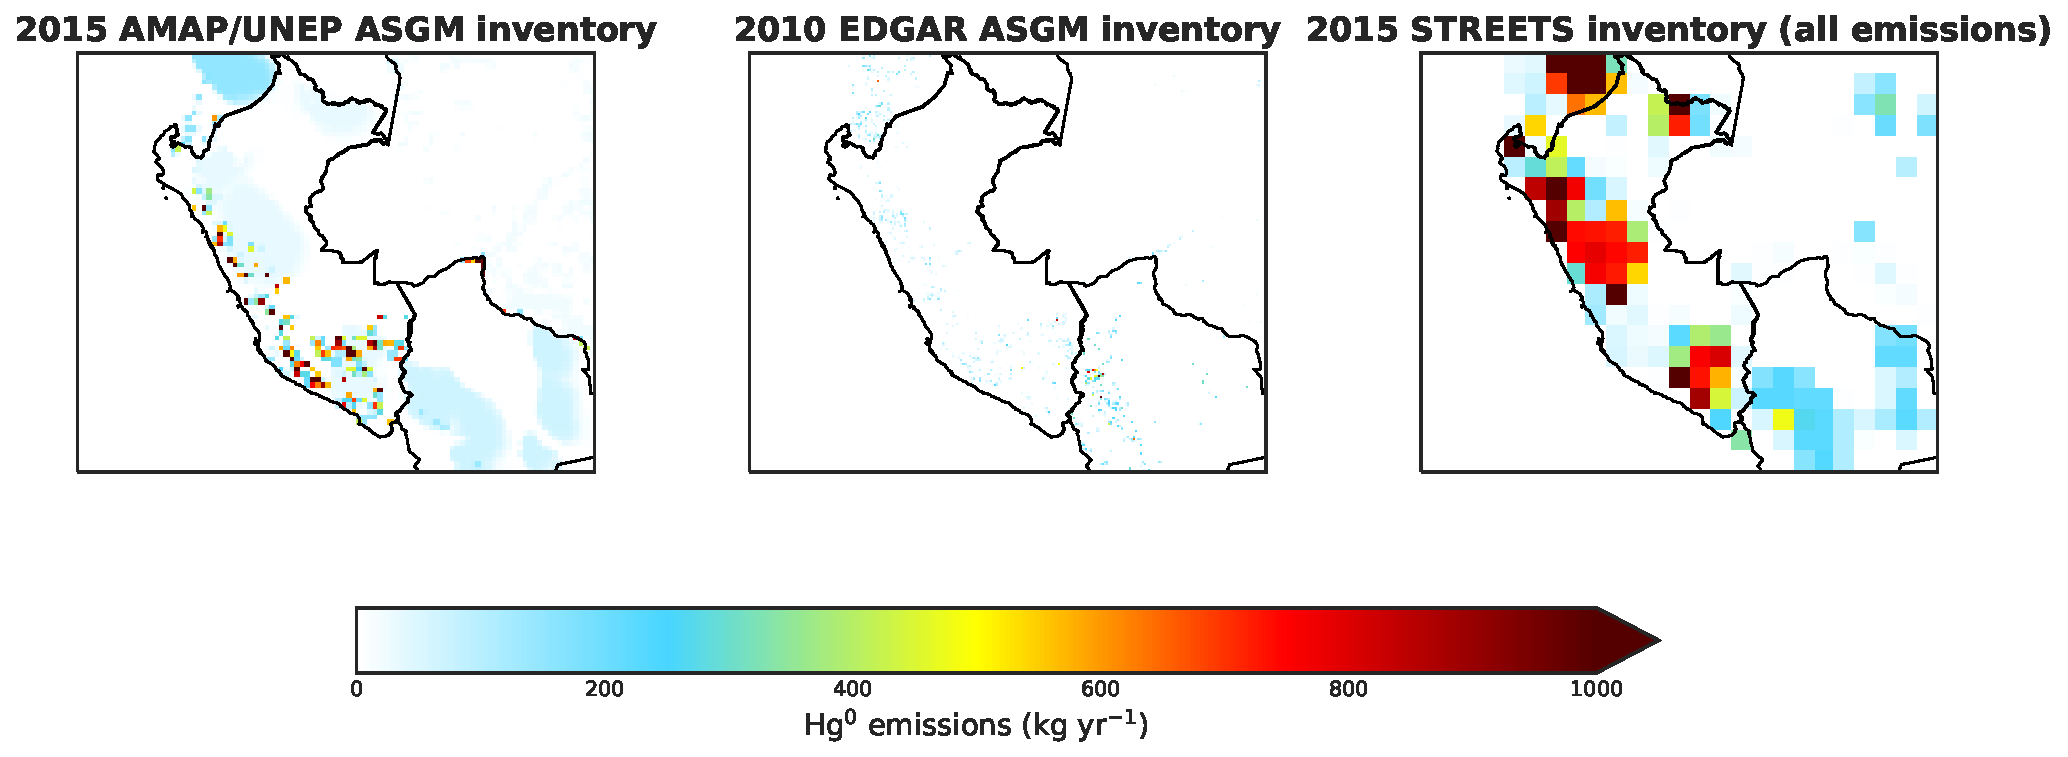
\includegraphics[width=\textwidth]{templates/figures/Peru_Maps/Hg_inventories.pdf}
  \centering
  \caption{Comparison of Hg emission from Peru as estimated by different global inventories \cite{united_nations_environment_programme_technical_2019,steenhuisen_development_2019,muntean_evaluating_2018,streets_global_2019}}
  \label{fig:Hg_inventories}
\end{figure}
\FloatBarrier


\subsection{Emission Modification and \gc Simulations}
\begin{flushleft}
    Six more simulations were added to the \on and \off \gc simulations presented in Chapter 2. The first additional simulation was similar to the \on but was  conducted at a higher resolution. The other five simulations were sensitivity runs that used modified emission inventories corresponding to changes in emissions from one of the grid boxes in the case study region.
\begin{figure}[H]
\centering

\begin{tabular}[H]{c}

\subfloat[GMA 2015 Grid]{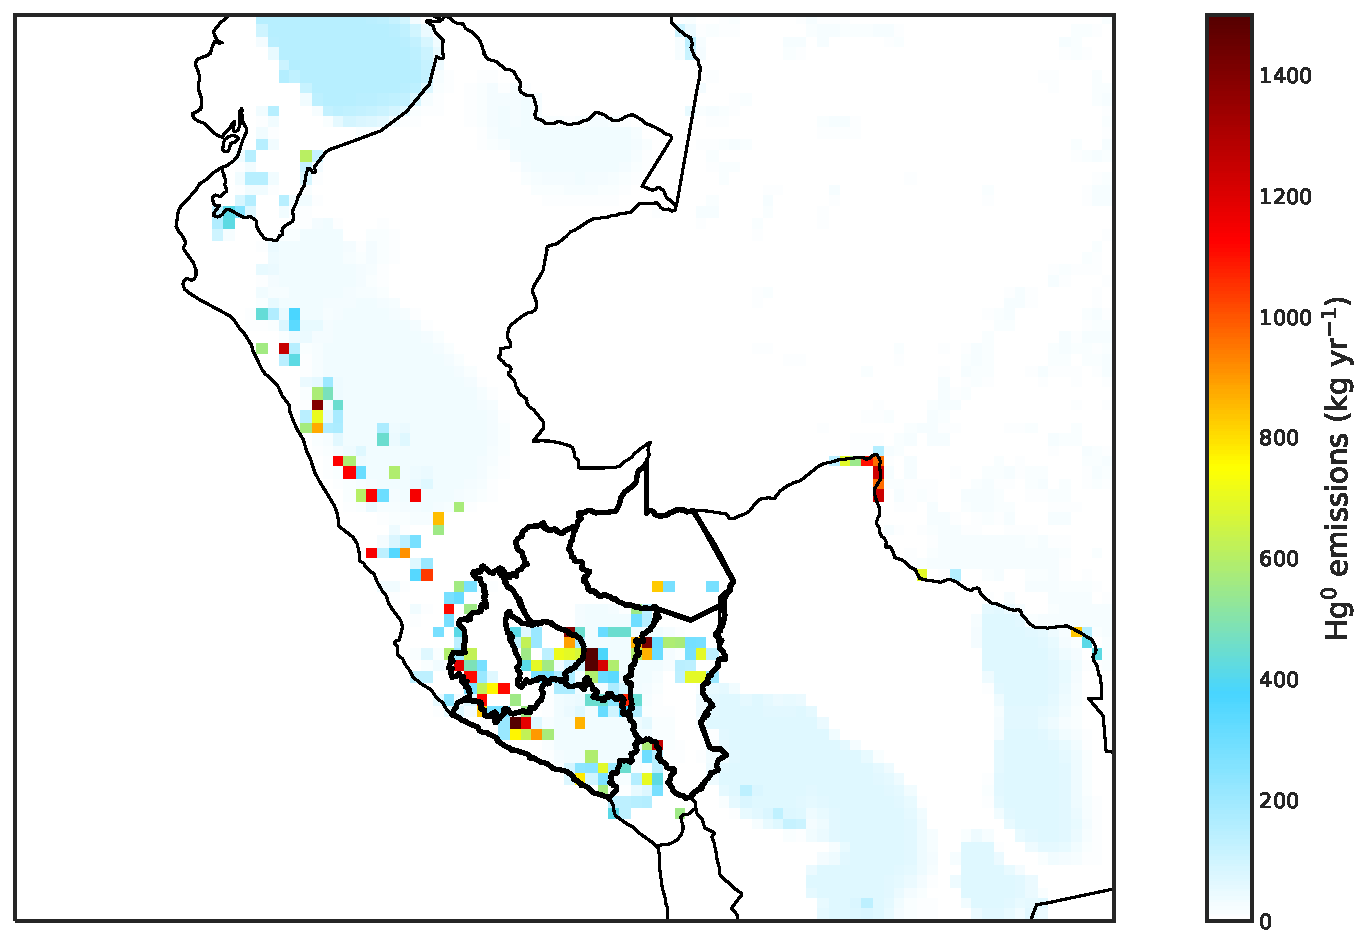
\includegraphics[width = 0.8\linewidth]{templates/figures/Peru_Maps/GMA2018inventory025x025.pdf}}\\
\subfloat[GEOS Chem Grid]{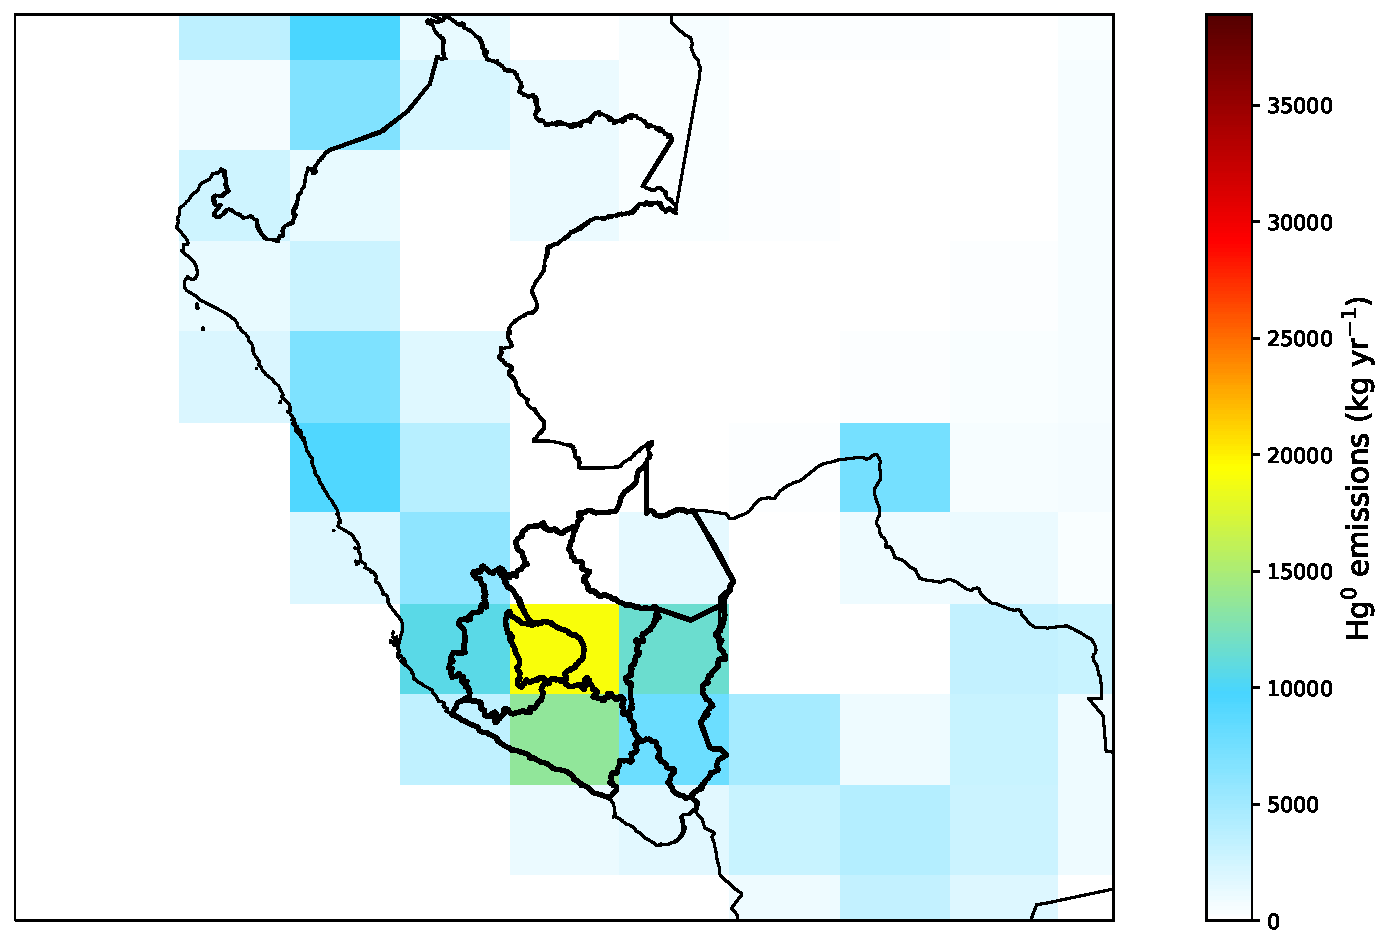
\includegraphics[width = 0.8\linewidth]{templates/figures/Peru_Maps/GMA2018inventory2x25.pdf}}


\end{tabular}
  

\captionof{figure}{Maps showing how the GMA2018 emission estimates for the year 2015 were distributed for Peru before re-griding (a) and after re-gridding to the \gc grid (b) }
\label{fig:GMA2018}
\end{figure}
\FloatBarrier
\end{flushleft}


\begin{table}[H]
\caption{Table showing the different GEOS-Chem simulations used in the analysis}
    \label{tab:all_geos_chem_simulations}
\begin{tabular}{lcp{0.5\linewidth}}

\textbf{Simulation Name}    &  Resolution       & \textbf{Description Estimate}                             \\
\hline
Base (ASGM=ON)              & 2.0$\times$2.5        & All Hg anthropogenic emission sources are turned on  \\
No ASGM (ASGM=OFF)          & 2.0$\times$2.5        & All ASGM emissions are turned off                     \\
Mdd                         & 2.0$\times$2.5        & Emissions from the \gc grid box located in  Madre de Dios  were scaled up by a factor of 2 \\

Apr                         & 2.0$\times$2.5        & Emissions from the \gc grid box located in Apurimac were scaled down by a factor of 0.5\\

Aqp                         & 2.0$\times$2.5        & Emissions from the \gc grid box located in Arequipa department were scaled up by a factor of 2\\

Npun                        & 2.0$\times$2.5        & Emissions from the \gc grid box located in the northern region of Puno were scaled up by a factor of 2 \\

Spun                        & 2.0$\times$2.5        & Emissions from the \gc grid box located in the southern region of the Puno were scaled up by a factor of 2 \\
\hline
\end{tabular}
\centering
\end{table}

\newpage
\subsection{Simulated Atmospheric Mercury Concentration Signals}
\begin{flushleft}
The relationship between the \hg emissions from a specific grid box and the \gc simulated atmospheric \hg concentration at distant points from the emissions source is assumed to be defined by a linear function. This means that an increase in emissions is expected to result in an increase in the \hg concentration. Consequently, the relationship between emissions and concentrations can be represented by the following equation:


\begin{equation}
\label{doublingSig}
Hg^0_{sig(region)}=Hg_{m_0}+\small\frac{(Hg_{m_1} -Hg_{m_0})}{(m_1 -m_0)}(m_{(region)} -m_0)
\end{equation}
where:
\end{flushleft}

\begin{description}[leftmargin=!,labelwidth={5 em}]
    \item [$region$] is the location of the emission source within the case study region.
    \item [$Hg^0_{sig(region)}$] is the simulated \hg concentration at the observation site due to $m_{(region)}$ at the grid box in the specific $region $ of interest.
    \item [$Hg_{m_0}$] is the Hg concentration  at the observation site generated by the Base (ASGM =ON) simulation. 
    \item [$Hg_{m_1}$] is the Hg concentration  at the observation site generated by the $i^{th}$ region simulation $i$=Mdd,Apr,Aqp,Npun,Spun. 
    \item [$m_1$] is the amount of emissions in Mega grams after scaling the emissions from a specific grid box.
    \item [$m_0$] is the amount of emissions in Mega grams before scaling the emissions from a specific grid box.
\end{description}


% \begin{flushleft}
% $Hg_{sig(region)}$ gives the Hg concentration signal in the atmosphere that results from a unit change in the tonnes of emissions from a specific grid box. Therefore, $Hg_{sig(region)}$ was used to investigate the sensitivity of the observations to the different amounts of additional ASGM Hg emissions and the regional grid boxes. The Hg concentration in the atmosphere that results from a specific change in emissions from a particular grid box was calculated using Equation \ref{ysignal} below.
% \begin{equation}
% \label{ysignal}
% \small{Hg_{m(region)}} =Hg_{sig(region)}(m-m_o), 
% \end{equation}
% where:
% \end{flushleft}


% \begin{description}[leftmargin=!,labelwidth={1.5 em}]
    
%     \item [$m_0$] is the GMA 2018 ASGM emissions estimate in metric tonnes for the particular grid box corresponding to a place in the case study region
    
%     \item [$m$] is the amount of emissions, in metric tonnes, from a grid box required to produce $Hg_{m}$ concentration in the atmosphere
% \end{description}




% \begin{flushleft}
% For each grid box in the case study region, the emissions were modified from their original GMA 2018 estimates to new values based on Hg emission estimates produced by the Artisanal Gold Council(AGC)
% \end{flushleft}

\subsection{Observation Site Selection}

\begin{flushleft}
TGM and GEM observation data from different locations in Latin America were analyzed and compared to the \gc simulated \hg concentrations for those sites in Chapter 2. The \gc predictions for ASGM contributions to atmospheric Hg concentration were higher at the CHC, making it an excellent candidate to use as a reference for comparison with the modified \gc Hg concentration predictions. Moreover, this site is the closest monitoring site to Peru hence it is expected that it would be more likely to detect atmospheric \hg changes that result from the changes in Hg emissions from the case study region. The time series of the observed concentration at the CHC station between July 2014 and January 2016 is shown in Figure \ref{fig:chc_time_series}.
\end{flushleft}

\begin{figure}[H]
  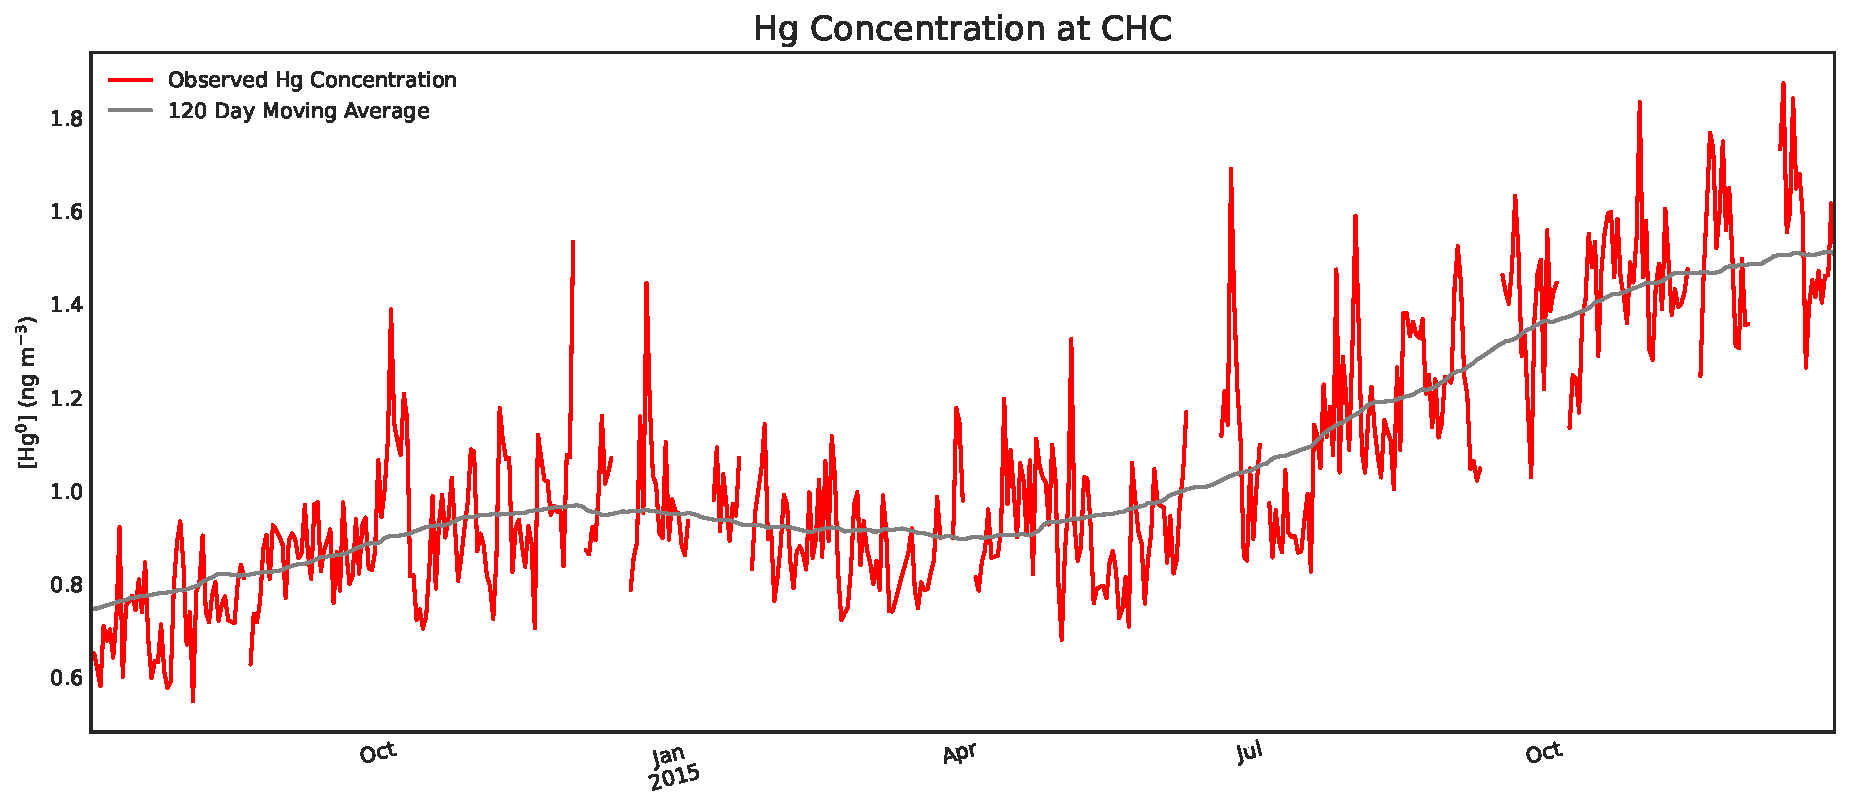
\includegraphics[width=\textwidth]{templates/figures/GMOS_Sites/ObsTimeSeries.pdf}
 
  \caption{The average daily TGM concentration at CHC in ng m\textsuperscript{-3} as a function of time over the measurement period from July 2014 to January 2016. The daily average concentration is indicated by the red line, while the grey line shows the 120-day moving average, which highlights the upward trend in the daily averages}
  \label{fig:chc_time_series}
  \centering
\end{figure}
\FloatBarrier
\begin{flushleft}

The detailed characteristics of the observations over this measurement period were described in Koenig et al. (2020); hence our analysis focused on using the observation TGM data to evaluate the performance of the GEOS-Chem model in predicting the \hg based on the input \hg emission inventories. As shown in Figure \ref{fig:chc_time_series}, the TGM concentration at CHC showed an upward trend, which Koenig et al. (2021) attribute to El Ni\~no-Southern Oscillation (ENSO)\cite{koenig_seasonal_2021}. As a result, they categorized the measured TGM concentrations in the atmosphere at the CHC site as normal conditions (NC), 2014-07 to 2015-05, and ENSO conditions 2015-06 to 2016-01. To reduce the number of records associated with ENSO, I limited my analysis to one year's worth of data from 2014-07 to 2015-07.
\end{flushleft}

\subsection{Markov Chain Monte Carlo}

\begin{flushleft}
The Markov-Chain Monte Carlo (MCMC) is a valuable sampling method for fitting models to data\cite{hogg_data_2018}. We apply the MCMC to constrain ASGM Hg emissions from the case study region in Peru.  The model is generated by a set of parameters and emissions, and we aim to sample from the parameters that best fit our data. The MCMC compares the modeled concentrations to the observed data using metrics such as the \nft confidence interval, mean, and the \iq. The MCMC generatively models given data by sampling around optimum values from the posterior distribution. The MCMC is a Bayesian approach; hence it requires the definition of priors on the parameters of interest. The priors encode information that we already know of the system. The probability of the model given the observed data is given by the posterior probability, $P(\theta|D)$, which is calculated using the Bayes theorem:

\begin{equation}
\label{bayes_eq}
P(\theta|D)=\frac{P(D|\theta)P(\theta)}{P(D)}
\end{equation}
where:
\end{flushleft}

\begin{description}[leftmargin=!,labelwidth={3 em}]
    \item [$P(D|\theta)$] is the likelihood which is the probability of the data given the model
    \item [$P(\theta)$] is the prior, which is the probability of the model and 
    \item [$P(D)$] is the evidence which is the probability of the data.
\end{description}

\begin{flushleft}
The MCMC enables the estimation of the sampling of the posterior distribution, which is the left-hand side of Equation~\ref{bayes_eq}. The MCMC is set up by following a set of steps that include defining a function that outputs a model given a set of input parameters and establishing an ensemble of walkers defined by a $\theta$ vector that contains a set of parameters from the model generating function. For the model generating function, the Hg concentration at a particular grid box is defined as a linear combination of Hg concentration signals from the case study region and the baseline Hg concentration produced by the \on as shown in the Equation \ref{Hg_conc} below:

\begin{align}
\begin{split}\label{Hg_conc}
Hg_{conc}= {}&Hg_{m(MdD)}+ Hg_{m(S-Puno)} + Hg_{m(N-Puno)} + Hg_{m(Apr)}+ Hg_{m(Aqp)}\\
            & +Hg_{m_0}
\end{split}
\end{align}

where:
\end{flushleft}

\begin{description}[leftmargin=!,labelwidth={5 em}]
    \item [$Hg_{m(MdD)}$] is the Hg concentration signal resulting from emissions from the Madre de Dios (MdD) grid box
    \item [$Hg_{m(S-Puno)}$] is the Hg concentration signal resulting from emissions from the South Puno (S-Puno) grid box
    \item [$Hg_{m(N-Puno)}$] is the Hg concentration signal resulting from emissions from the North Puno (N-Puno) grid box
    \item [$Hg_{m(Apr)}$] is the Hg concentration signal resulting from emissions from the Apurimac (Apr) grid box
    \item [$Hg_{m(Aqp)}$] is the Hg concentration signal resulting from emissions from the Arequipa (Aqp) grid box
    \item [$Hg_{m_0}$] is the baseline Hg concentration signal.
\end{description}

\begin{flushleft}
Each of the $Hg_{m(region)}$ terms of Equation \ref{Hg_conc} represent signals from the different departments are calculated using Equation~\ref{doublingSig}. The $m_(region)$ terms are the only unknowns and the equation can be expanded to isolate the terms with $m_(region)$, which is the parameter we are optimizing for in the MCMC method. The expanded form of Equation \ref{Hg_conc} is shown below:

\begin{align}
\begin{split}\label{Cs36PoGd2l}
Hg_{conc}={}& (m_{(MdD)}Hg_{sig_{(MdD)}} -m_oHg_{sig_{(MdD)}})+ (m_{(S-Puno)}Hg_{sig_{(S-Puno)}} -m_oHg_{sig_{(S-Puno)}}) \\
            &+ (m_{(N-Puno)}Hg_{sig_{(N-Puno)}} -m_0Hg_{sig_{(N-Puno)}}) + (m_{(Apr)}Hg_{sig_{(Apr)}} -m_oHg_{sig_{(Apr)}}) \\
            &+ (m_{(Aqp)}Hg_{sig_{(Aqp)}} -m_oHg_{sig_{(Aqp)}})+Hg_{m_0}
\end{split}
\end{align}

Since the values of $m_{(region)}$ are the parameters that we want to estimate using MCMC, they can be represented as $\theta_i=m_{(region)}, i=1$ and the other terms, including the background concentration, are combined into one constant, C:

\begin{equation}
\begin{aligned}
    Hg_{conc}  & = \theta_0C  + \theta_1Hg_{sig_{(MdD)}}+ \theta_2Hg_{sig_{(S-Puno)}} +  \theta_3Hg_{sig_{(N-Puno)}} \\
                & \ \ \ \  +\theta_4Hg_{sig_{(Apr)}} +  \theta_5Hg_{sig_{(Aqp)}}
\end{aligned}
\end{equation}

\begin{align}
Hg_{conc} =\begin{bmatrix} C & Hg_{sig_{(MdD)}} & Hg_{sig_{(S-Puno)}} &Hg_{sig_{(N-Puno)}} &Hg_{sig_{(Apr)}} &Hg_{sig_{(Aqp)}}\end{bmatrix} \times 
            \begin{bmatrix} \theta_0 \\ \theta_1 \\ \theta_2\\ \theta_3\\ \theta_4\\ \theta_5  \end{bmatrix}
\end{align}
where $\theta_0=1$ and $Hg_{conc}$ is the modeled Hg concentration at the observation site of interest.
\end{flushleft}

\begin{flushleft}
Next, the metrics being compared to their observed counterparts are calculated to be used in Equation \ref{model_definition} during the MCMC simulation. 
\end{flushleft}

% \begin{align}
% \begin{split}\label{model_definition}
% \hat{y}= {}&Hg_{m(MdD)}+ 
% \end{split}
% \end{align}


\newpage
\section{Results and Discussion}
\subsection{National vs. Global Mercury Inventory}
Figure \ref{fig:agc_vs_gma18} compares ASGM Hg emissions estimates from two different bottom up inventories regrided to the GEOS-Chem 2$\times$2.5 grid used in the simulations in this study. The GMA 2018 2015 estimates for Hg emissions from ASGM activities in Peru as distributed by Steenhuisen and Wilson\cite{steenhuisen_development_2019} are shown in Figure \ref{fig:agc_vs_gma18},(a). Furthermore, Figure \ref{fig:agc_vs_gma18},(b) represents my interpretation of how the Peru ASGM Hg emissions estimates from the Artisanal Gold Council's(AGC) inventory\cite{agc_reporte_2017} would be mapped on to the GEOS Chem Grid. The estimates for the total ASGM emissions from Peru are almost similar in both inventories, 110.4 t/y in the GMA 2018 and 108.74 t/y in the AGC national inventory.

% \begin{figure}[H]
% \centering

% \begin{tabular}[H]{cc}

% \subfloat[]{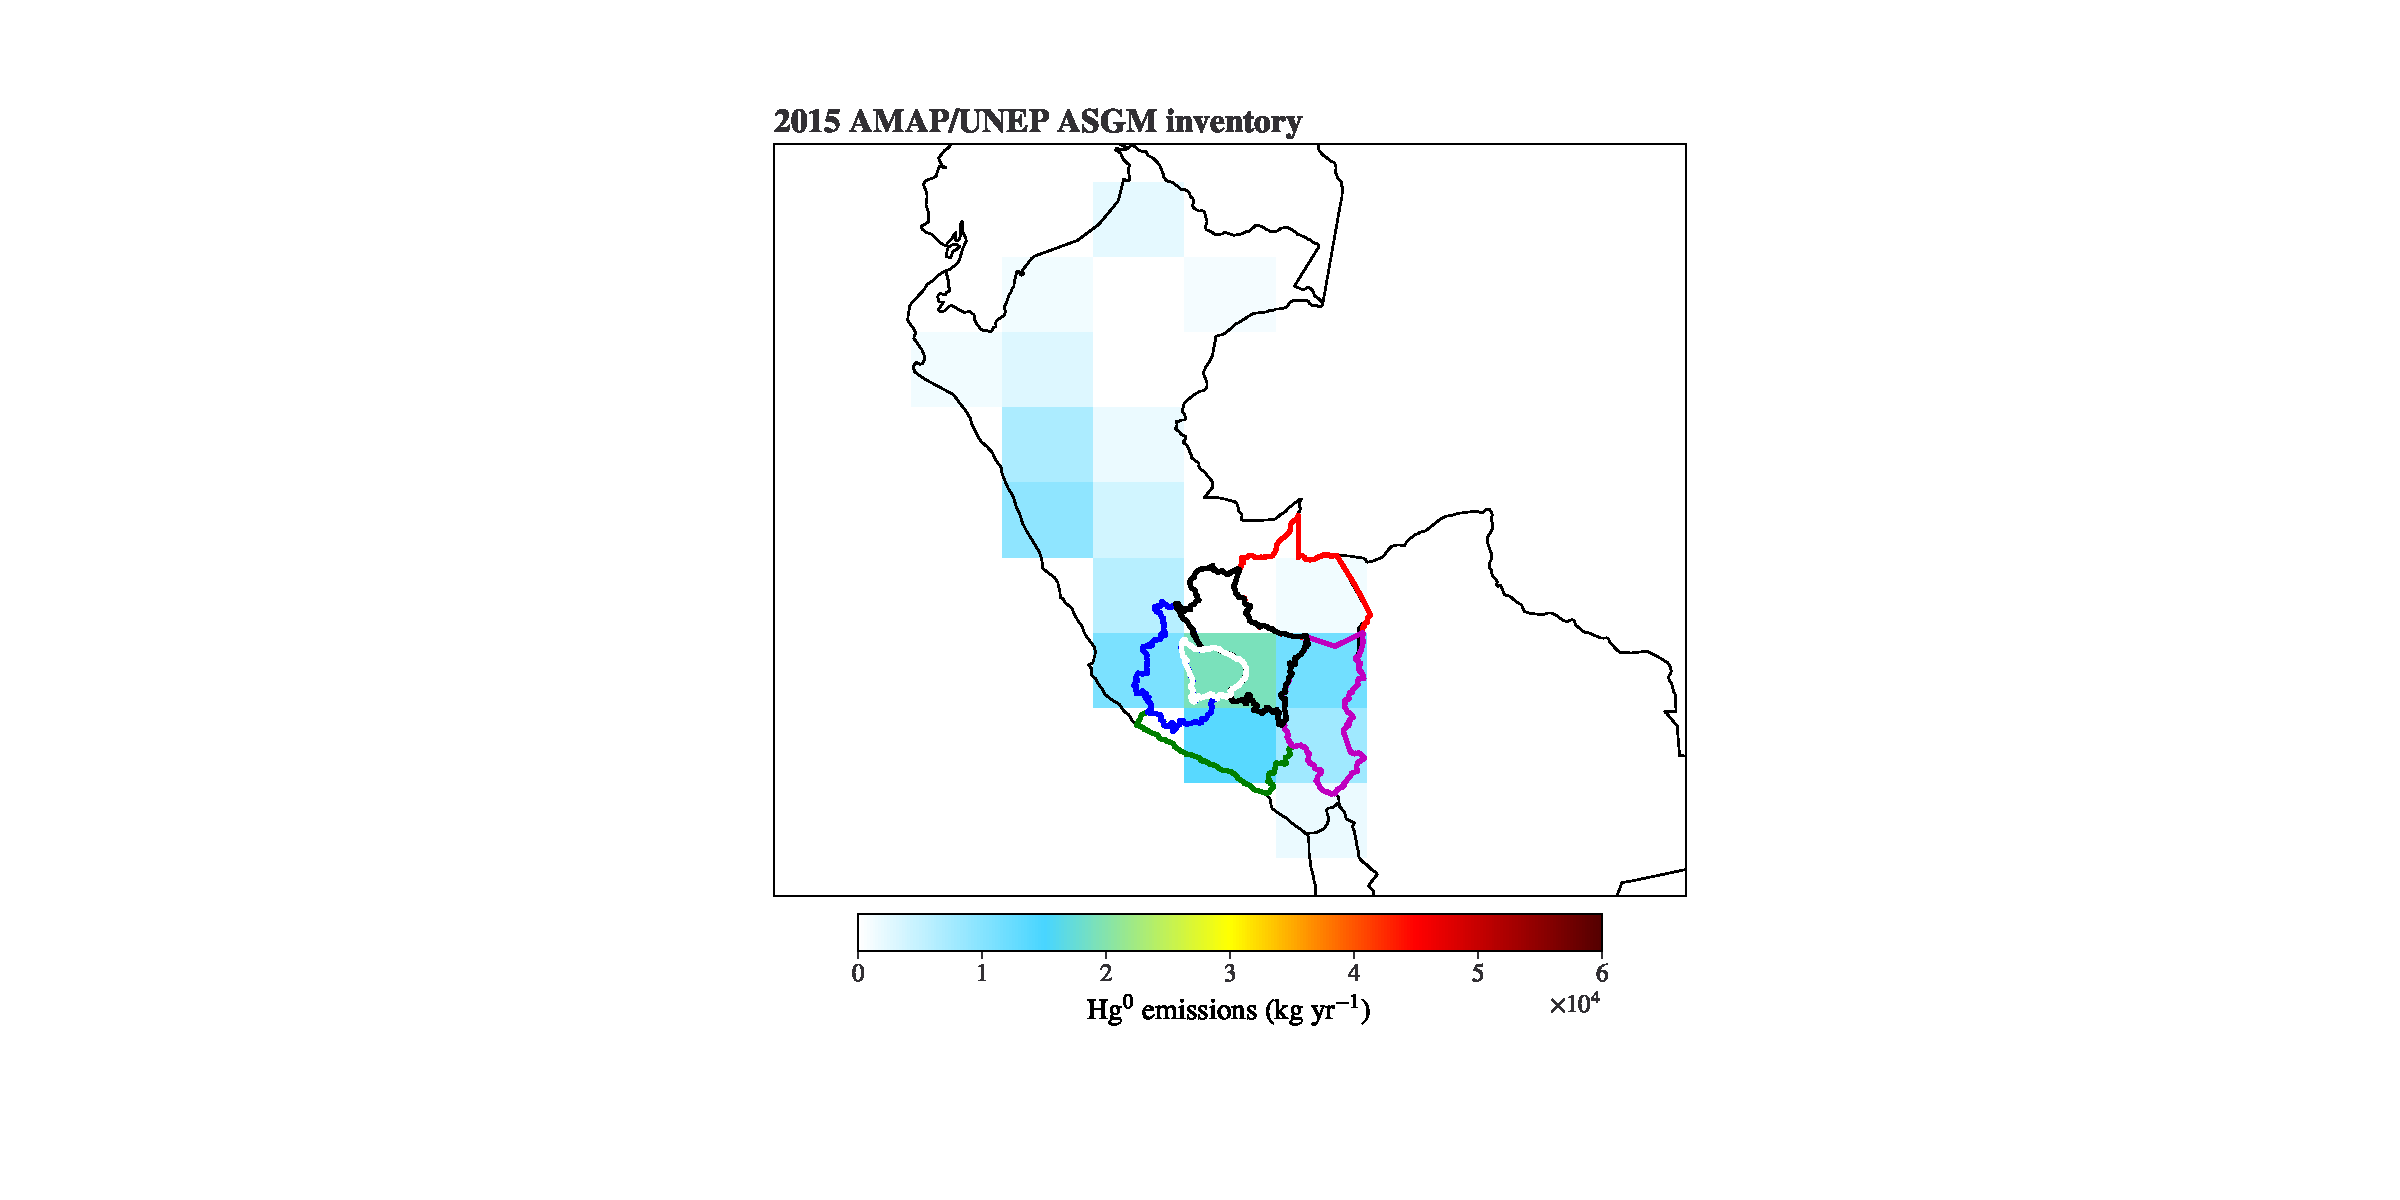
\includegraphics[width = 0.5\linewidth]{templates/figures/Peru_Maps/GMA2018inventory2x25Peru.pdf}}
% \subfloat[]{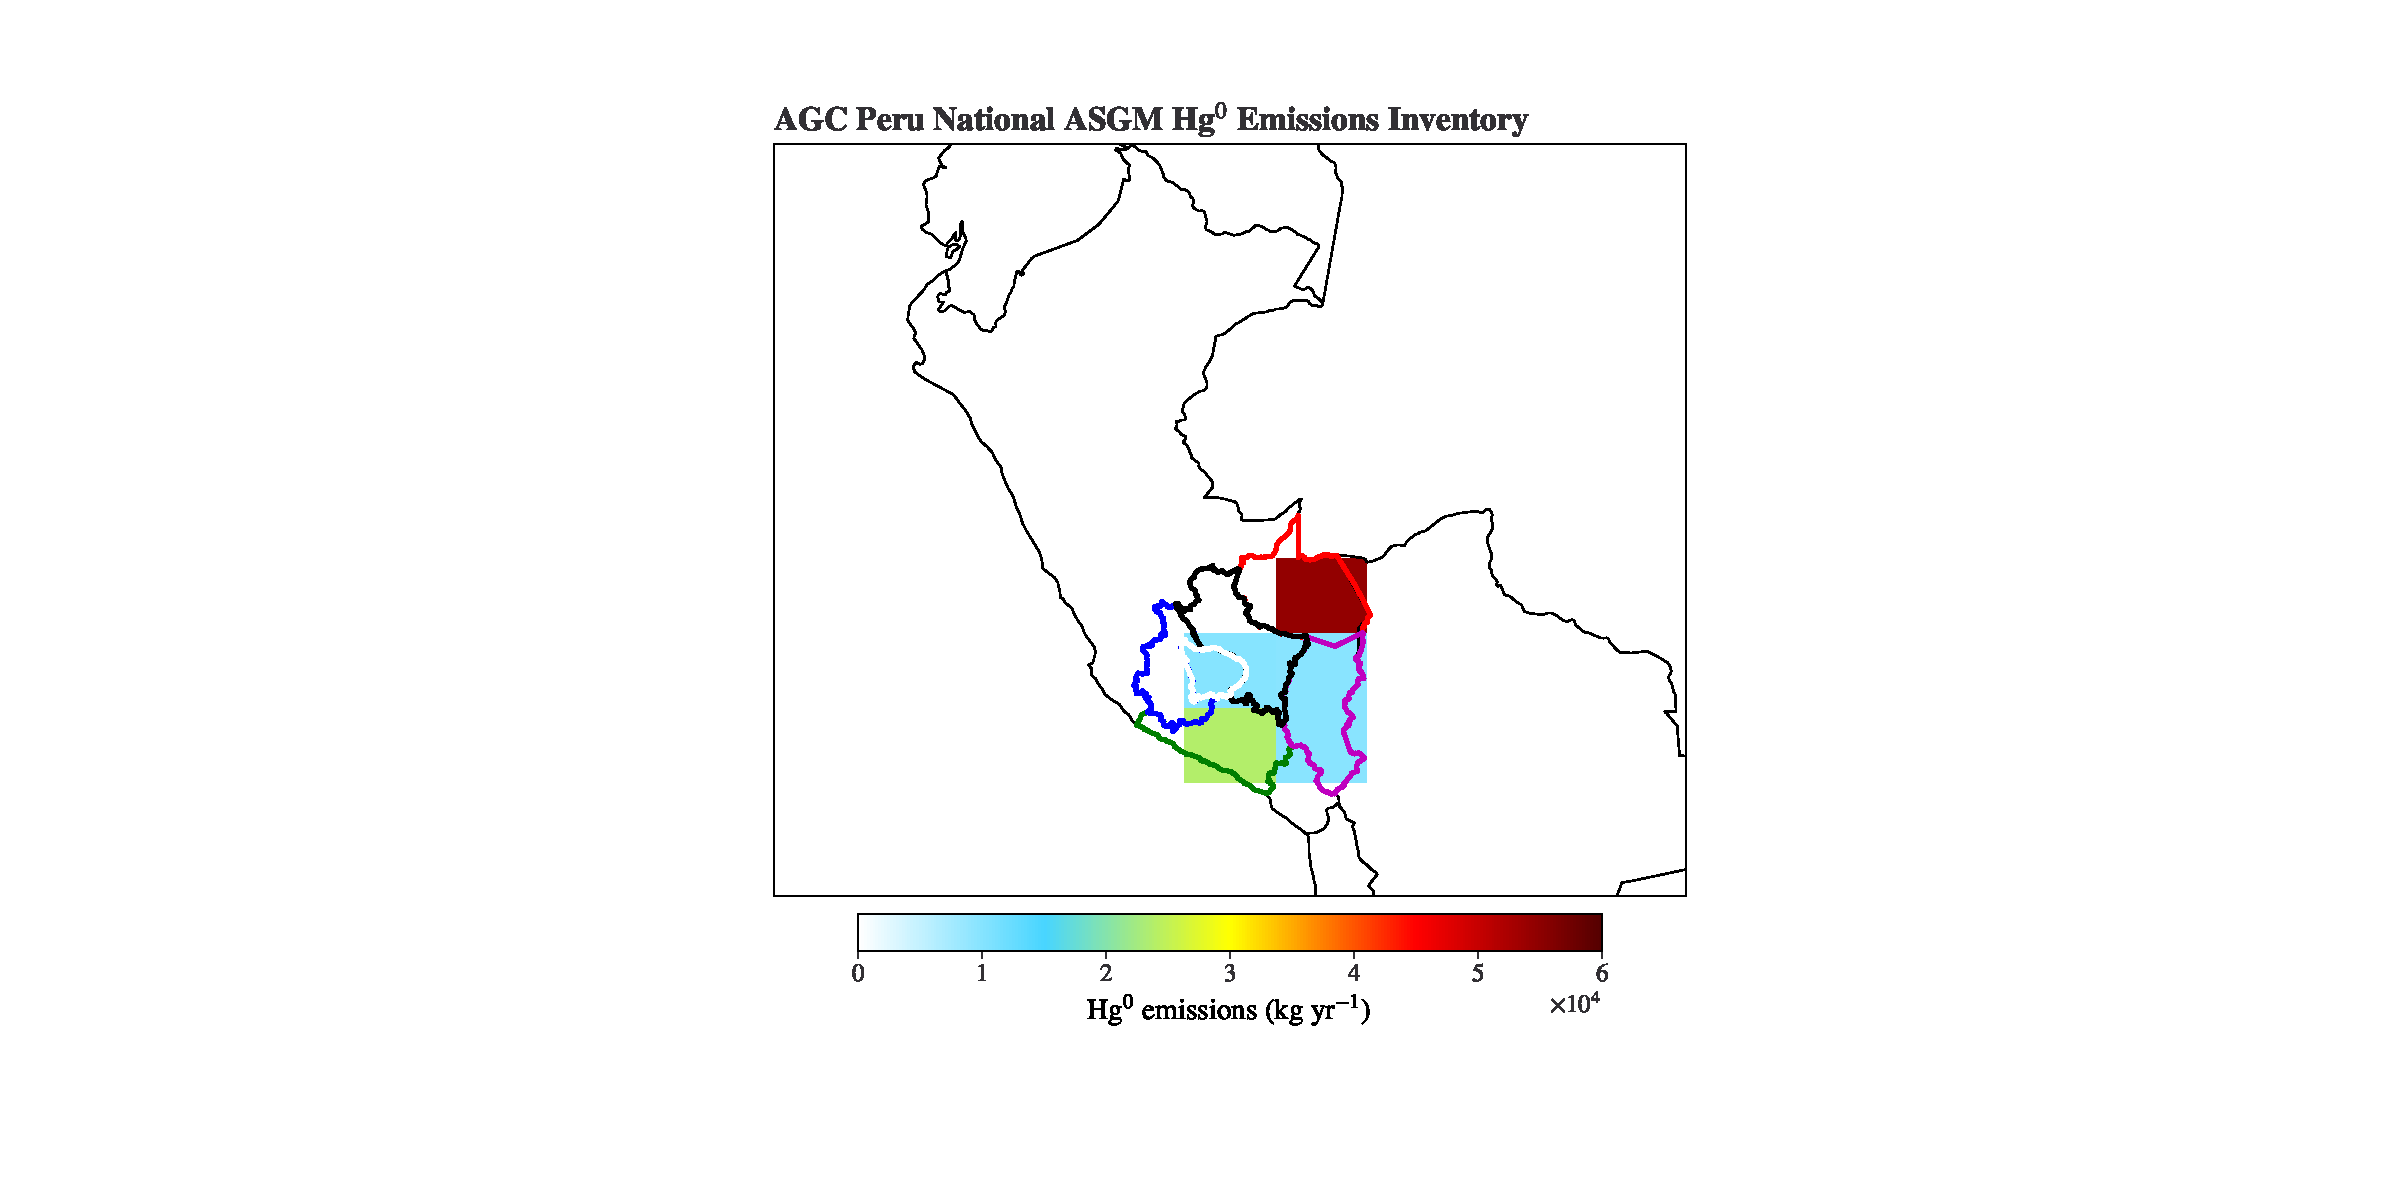
\includegraphics[width = 0.5\linewidth]{templates/figures/Peru_Maps/AGCinventory2x25Peru.pdf}}\\


% \end{tabular}
\begin{figure}[H]
\centering
  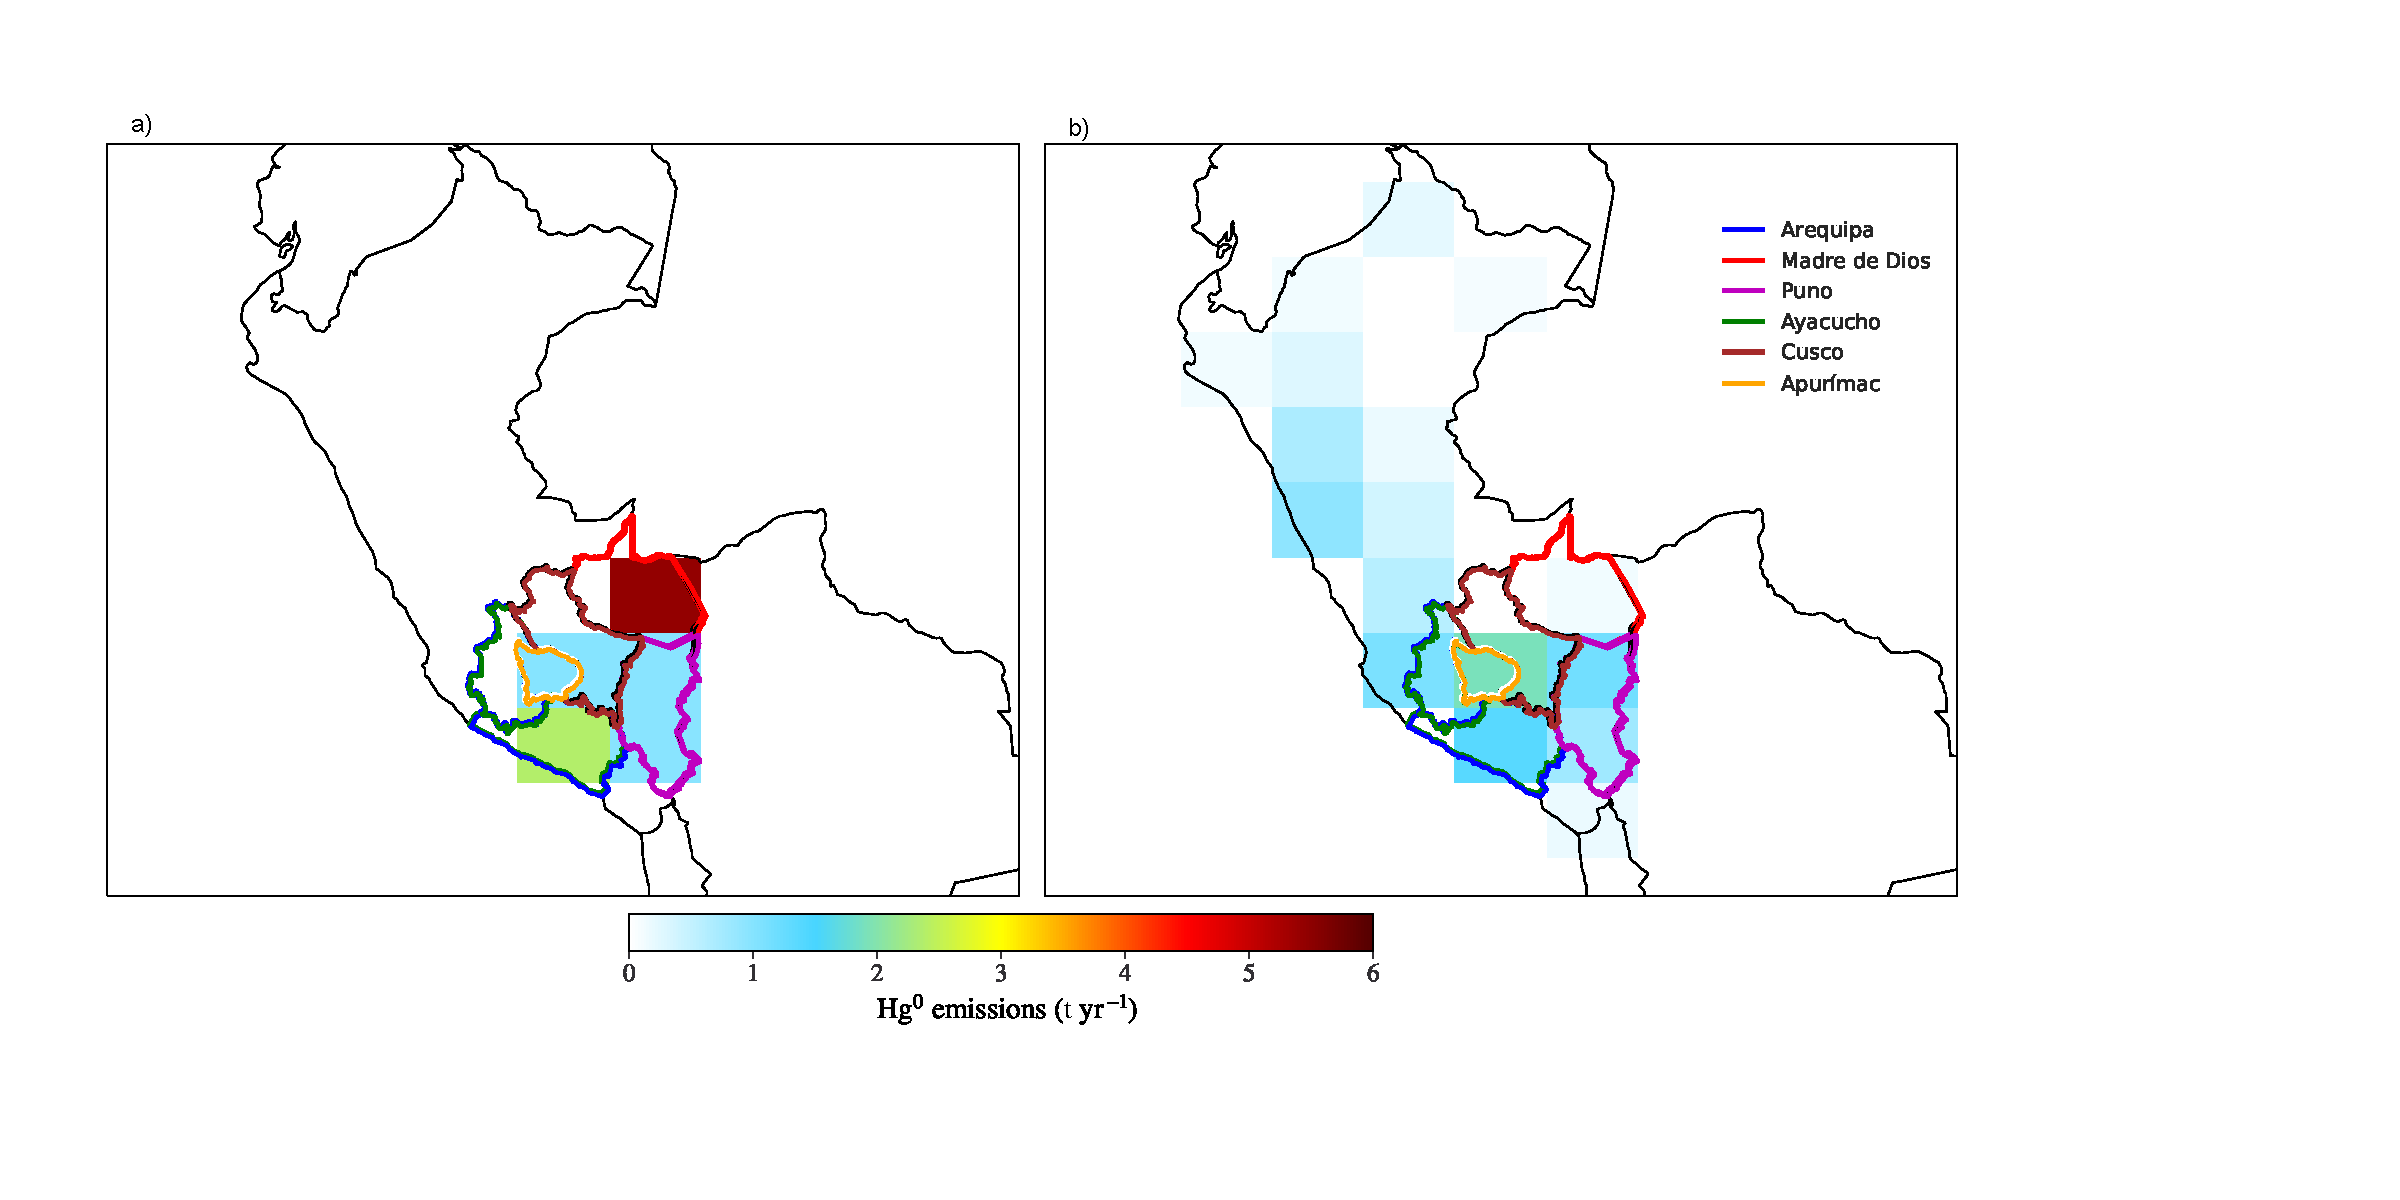
\includegraphics[width=\textwidth]{templates/figures/Peru_Maps/comparison_AGC_GMA18.pdf}  

\captionof{figure}{The AGC Peru National ASGM Hg emissions inventory as published in \cite{agc_reporte_2017} and regridded to the GEOS-Chem 2$\times$2.5 grid resolution is shown in (a).How the ASGM Hg emissions in Peru were distributed in two bottom-up inventories. The GMA2018 ASGM Hg emissions inventory for 2015 as distributed in \cite{steenhuisen_development_2019} and regridded  to the GEOS-Chem 2$\times$2.5 grid resolution is shown in (b).}
\label{fig:agc_vs_gma18}
\end{figure}
\FloatBarrier
\begin{flushleft}
The AGC's Peru national inventory attributed most of the ASGM Hg emissions to the South Eastern departments in the country\cite{agc_reporte_2017}. As seen in Table\ref{tab:agc_vs_gma18}, the Madre de Dios department is the largest source of Hg emissions, followed by Arequipa,Puno, Ayacucho, Cusco, respectively. The rest of Peru together contributes about 0.98 tonnes of Hg emissions annually. Contrary to the AGC's method, Steenhuisen and Wilson (2019) based the Hg emissions spatial distribution on a proxy based on the likelihood of gold occurrence in soils, sediments, and bedrock and knowledge of actual ASGM activity. For Peru, they used the global alluvial gold map and a (gold) mining concessions dataset, which includes large-scale mining. Considering that the AGC estimate was developed in line with the requirement of the NAP process, I assumed it is more reflective of the ground truth. Furthermore, the Madre de Dios is a well known ASGM hotbed in Peru and within the Amazon region hence the GMA 2018 estimate of Hg emissions of 1.39 t/y can be easily identified as inaccurate. Both inventories are essential and complement each other. The AGC's inventory gives a baseline of the amount and distribution of ASGM Hg emissions at the national level but does not show the influence of the emissions at the regional and global levels. On the other hand, the global inventory is a source of information about local, regional and global emissions. 
\end{flushleft}
\begin{flushleft}
    The global and national inventory differences informed the hypothesis that incorrect emissions parameterization in \gc may be why the \on does not reproduce the observed atmospheric concentrations. The following sections present the results from the analysis where the emissions from the departments in the case study were scaled to compare with observations and produce top-down estimates of Hg emissions for the case study region.
\end{flushleft}
\setlength{\tabcolsep}{5pt}
\begin{table}[H]
  \begin{center}
    \caption{Comparison of ASGM Hg emissions from Peru as published in the GMA2018 inventory for 2015 and the Peru national inventory of ASGM emissions in the case study region. The emissions are in t/year, and the right-most column shows the percentage difference between the AGC and GMA 2018 Hg emissions estimates }
    \label{tab:agc_vs_gma18}
    \begin{tabular}{lrrr}
       %<-- added & and content for each column
      
    \textbf{Region}     & \textbf{AGC}      & \textbf{GMA 2018}             & \textbf{Percentage Difference}       \\
                        & (t$\cdot y^{-1}$) & (t$\cdot y^{-1}$)                    &        (\%)\\
\hline    
    Madre de Dios       & 54.46             & 1.39                          &    -97.45       \\
    Puno                & 19.37             & 19.42                         &    +0.26     \\
    Arequipa            & 23.86             & 18.99                         &    -20.41       \\ % <--
    Apurimac            & 0.03              & 19.32                         &    +64300.00    \\
    Ayacucho            & 9.15              & 8.99                          &    -1.75           \\ % <--
    Cusco               & 0.89              & 0.04                          &    -95.50           \\
    Rest of Peru        &  0.98             & 42.25                         &    +4211.22        \\
   
    \hline
    \textbf{Total}           &110.4             &108.74     &        \\
    \end{tabular}
  \end{center}
\end{table}

\subsection{GEOS-Chem Predictions vs. Observations at Chalcataya}
\begin{flushleft}
The comparison of the \gc predicted \hgc to observed TGM at CHC for the one-year period from 2014/07/03 to 2015/07/03 is shown in Table \ref{tab:ModelvsObsStats}. The metrics being compared on the table are the mean ($\mu$), standard deviation ($\sigma$), interquartile range(\iq), Spearman correlation ($r_s$) and Pearson correlation ($r$).The mean \hg concentration produced by the \off  was within 1\% of the observed TGM concentration as seen in Table \ref{tab:ModelvsObsStats}. On the contrary, the average \hg produced by the \on overestimated the mean by 29\%.
\end{flushleft}
\setlength{\tabcolsep}{3.5pt}
\begin{table}[H]
  \begin{center}
    \caption{Characteristics of observed and modeled Hg concentration in CHC where $\mu$ is the annual average Hg concentration, $\sigma$ is the standard deviation, \iq is the interquartile range, $r_s$ is the Spearman correlation, $r$ is the Pearson correlation }
    \label{tab:ModelvsObsStats}
    \begin{tabular}{lccccc}
       %<-- added & and content for each column
      
                            & $\mu$                 & $\sigma$              & \iq                & & \\
                            &  (ng m$^{-3}$)/year)  & (ng m$^{-3}$)/year)   & (ng m$^{-3}$)/year)   & & \\
     \cmidrule{2-4}
     Observations           & 0.90                  & 0.16                  & 0.18                  &  & \\
     \textbf{Simulations}   &                       &                       &                       &\textbf{$r_s$} &\textbf{$r$} \\ %
      \hline
      No ASGM (ASGM=OFF)    & 0.91                  & 0.06                  & 0.11                  & 0.170          & 0.144        \\ 
      Base (ASGM=ON)        & 1.16                  & 0.14                  & 0.20                  & 0.124         & 0.101         \\ % <--
    \end{tabular}
  \end{center}
\end{table}
\FloatBarrier
\begin{flushleft}
   Figure \ref{fig:ModelvsObsNstats} shows a detailed comparison of the simulated \hg concentration and the observed TGM concentration at CHC. The observations (in red) are plotted as a function of time in plots (a) and (c) with the \off (in green) in plot (a)  and the \on in (blue) in plot (c). The scatter plots in (b) and (d) represent the modeled \hg  as a function of the measured TGM concentration. The scatter plot in (b) shows that the variability in the observed TGM concentration is not captured by the \off, while the scatter plot in (d) shows that the \on overestimates the observed TGM concentration values. However, the \on closely approximates the variability in the observed Hg concentration as its standard deviation is only 12.5\% less than the observation standard deviation, yet the \off standard deviation is 62.5 \% less than the observation standard deviation. These results mirror Chapter 2 results, where the entire CHC dataset was compared to the modeled \hgc at CHC even though here the dataset has been truncated to the one-year period from 2014/07/03 to 2015/07/03. 
\end{flushleft}
\begin{figure}[H]
  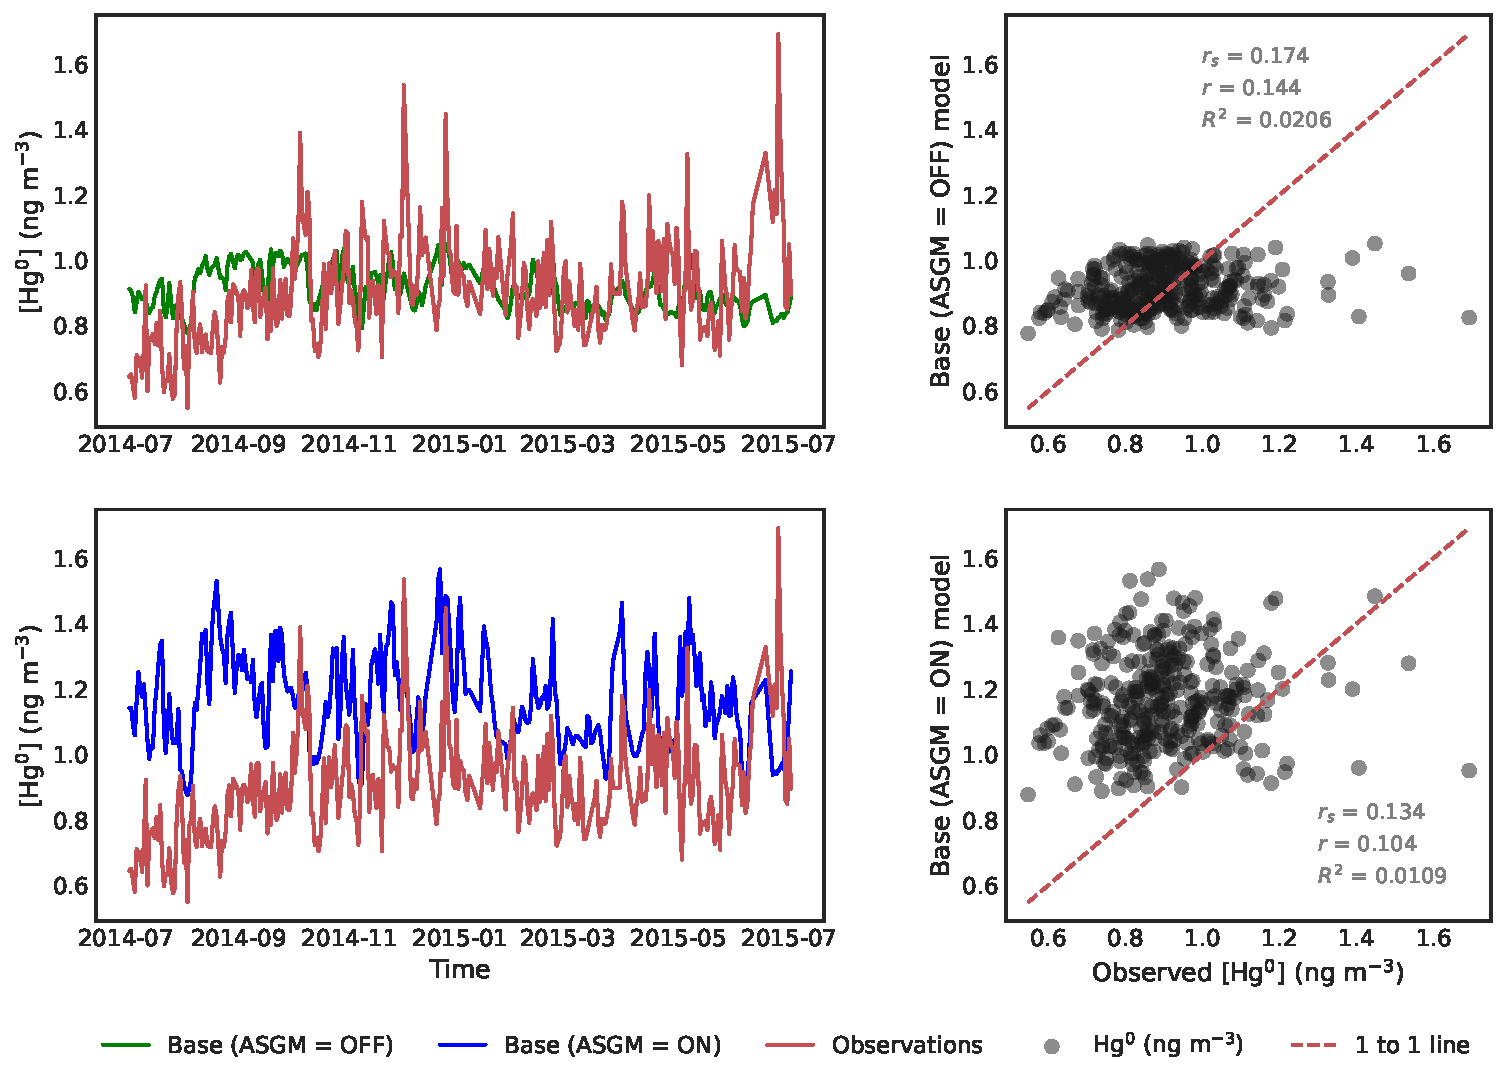
\includegraphics[width=0.85\textwidth]{templates/figures/ModelvsObs/TimeSeriesNsactter_obsVmodel_v1.pdf}
  \centering
  \caption{The observations (in red) are plotted as a function of time in plots (a) and (c) with the \off (in green) in plot (a) and the \on in (blue) in the plot (c). Analysis of the observed Hg concentrations vs. the \off  shows how the modeled mean closely approximates the observed mean and poorly estimates the daily variability, as shown by the difference in the size of the daily spikes of the Hg concentrations. The scatter plots in (b) and (d) represent the modeled \hg  as a function of the measured TGM concentration.}
  \label{fig:ModelvsObsNstats}
\end{figure}
\FloatBarrier

\begin{flushleft}
    Even though GEOS-Chem closely approximated the mean Hg concentrations at CHC in the \off, the Spearman ($r_s$) and Pearson ($r$) correlations between the modeled and observed concentrations were very low at 0.17 and 0.144, respectively. Moreover, the coefficient of determination, $R^2$ between the observed and modeled concentrations in \off case was almost zero at 0.0207. This is in line with the general result in Chapter 2 that the model poorly estimates the observed Hg emission concentrations in the atmosphere. Brasseur and Jacob (p.471 2017) argue that in cases where a model captures the observed means but not the observed variability, the mean may be wrongly interpreted \cite{brasseur_modeling_2017}. The mean in the \off case assumes zero Hg emissions from ASGM hence its direct comparison with the observations may be interpreted as wrong the observed Hg concentration is influenced by ASGM Hg emissions. Furthermore, the model underestimates the observed Hg concentrations due to a poor definition of dry deposition or vegetation uptake.  
\end{flushleft}

\begin{flushleft}
However, the \on reproduces the \iq and 95th \% confidence interval better than it reproduces the mean, as seen in Figure \ref{fig:density_plots_noASGM_vs_ASGM_vsObs}. Density plots of the modeled and observed Hg concentration at Chalcataya are shown in Figure \ref{fig:density_plots_noASGM_vs_ASGM_vsObs}. In (a), the actual distributions for the two simulations and the observations are plotted where the observed TGM concentration distribution is shown in red, the distribution of the \hgc predicted by the \off is shown in green, and that produced by the \on is shown in blue. Figure \ref{fig:density_plots_noASGM_vs_ASGM_vsObs} (b) shows the identical distributions to (a) after standardization by subtracting the mean in each distribution to see how the shapes of the distributions compare with each other.  
\end{flushleft}



\begin{figure}[H]

\begin{tabular}[H]{cc}
\centering

\subfloat[]{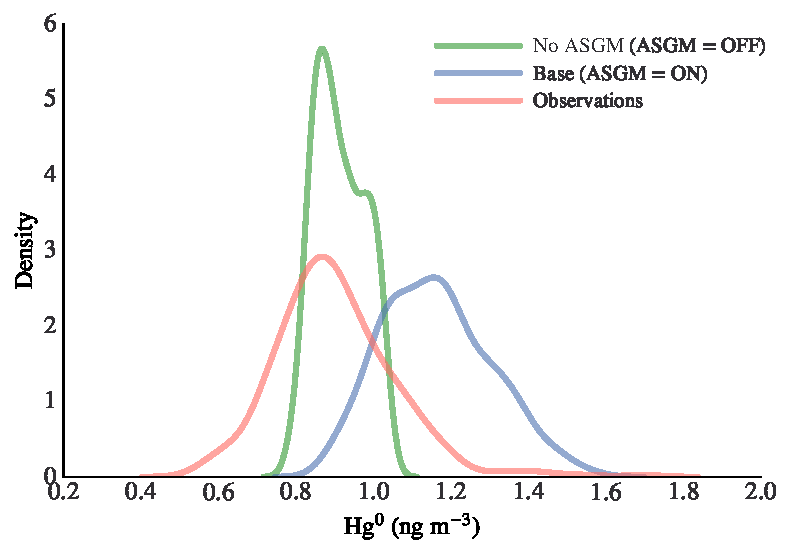
\includegraphics[width = 0.45\linewidth]{templates/figures/ModelvsObs/06-12-22_models_vs_observations_density-plot.pdf}} &
\subfloat[]{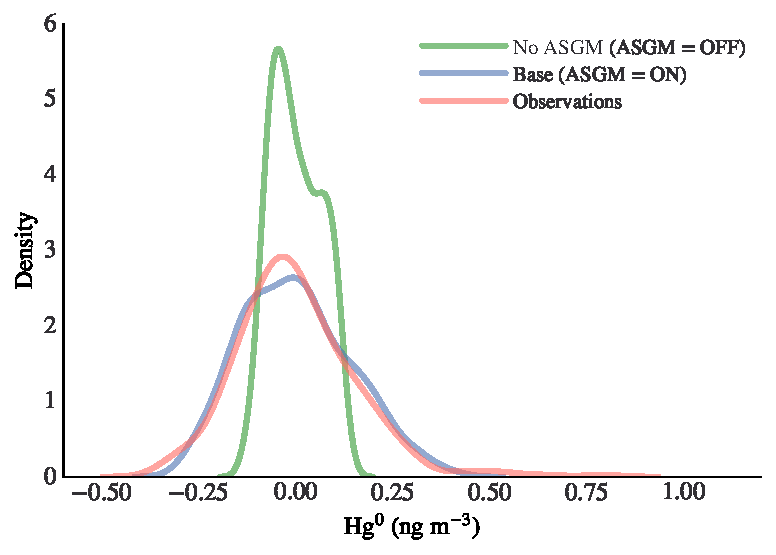
\includegraphics[width = 0.45\linewidth]{templates/figures/ModelvsObs/06-12-22_models_vs_observations_density-plot_std.pdf}}
\end{tabular}

\captionof{figure}{Density plots of the modeled and observed Hg concentration at Chalcataya. In (a), the actual distributions for the two simulations and the observations are plotted where the observed TGM concentration distribution is shown in red, the distribution of the \hgc predicted by the \off is shown in green, and that produced by the \on is shown in blue. In (b), the same distributions are shown after standardization by subtracting the mean in each distribution for easy comparison of the shapes of the distributions}
\label{fig:density_plots_noASGM_vs_ASGM_vsObs}
\end{figure}
\FloatBarrier
\begin{flushleft}
    Figure \ref{fig:density_plots_noASGM_vs_ASGM_vsObs}, b) shows how the \hgc produced by the \on have a distribution that is similar to the distribution of the observations in terms of standard deviation, \iq and \nft. The \off produced \modelc which shows no instance of high \hg concentrations at CHC, and the high concentrations are only produced by the \on. These density plots inform us that the range of observed Hg concentrations in the atmosphere at CHC is primarily influenced by ASGM emissions. Consequently, metrics such as the standard deviation, \iq, and \nft may provide better information about ASGM Hg emission's influence on the observed Hg concentration in the atmosphere than the mean.
\end{flushleft}
\newpage
\subsection{Comparison of Observations with Emission Modification}
\begin{flushleft}
The sensitivity of the modeled \hgc at CHC to the changes in Hg emissions from each grid box in the case study region was investigated by finding the mean, \iq, and correlation as functions of the emissions from each specific grid box. Figure \ref{fig:mean_of_signals_vs_emissions_per_site} shows the plots of the relationship between the means of \modelc as a function of Hg emissions from the grid box corresponding to the respective regions in the case study. The means of \modelc for a given amount of Hg emissions from each grid box are compared to the red horizontal line, which indicates the value of the mean of the observed TGM concentration of 0.90 as presented in Table \ref{tab:ModelvsObsStats}. 
\end{flushleft}

\begin{flushleft}
Moreover, the blue dashed line shows the linear regression line for the values of \modelc as a function of the Hg emissions. All the plots show that the mean of the Hg concentration changes linearly with an increase in emissions and have a $R^2$ value of 1, which means that the percentage variation in the mean of \modelc is explained by the relationship between the emissions and the mean of \modelc. 
%The effect of reducing emissions from each site was explored through the negative values of Hg emissions, and it did not lead to mean Hg concentration values that matched the mean of the observed concentration at CHC for the range of emission reductions explored.
\end{flushleft}
\begin{figure}[H]

\begin{tabular}[H]{cc}
\centering

\subfloat[South Puno]{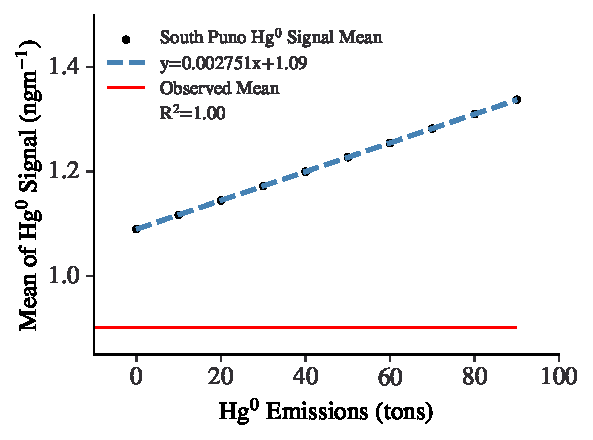
\includegraphics[width = 0.45\linewidth]{templates/figures/individual_site_modifications/mean_Spun_sigs.pdf}} &
\subfloat[North Puno]{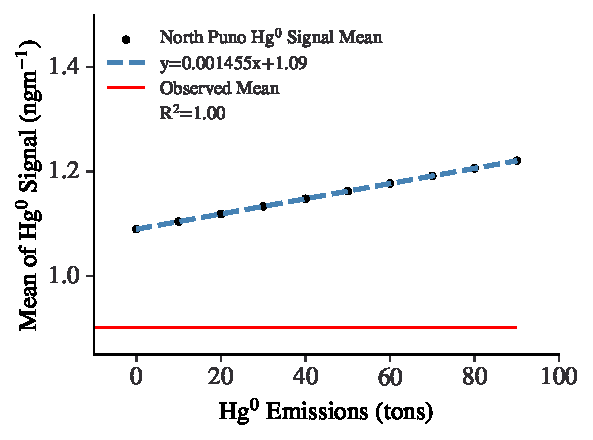
\includegraphics[width = 0.45\linewidth]{templates/figures/individual_site_modifications/mean_Npun_sigs.pdf}}\\
\subfloat[Arequipa]{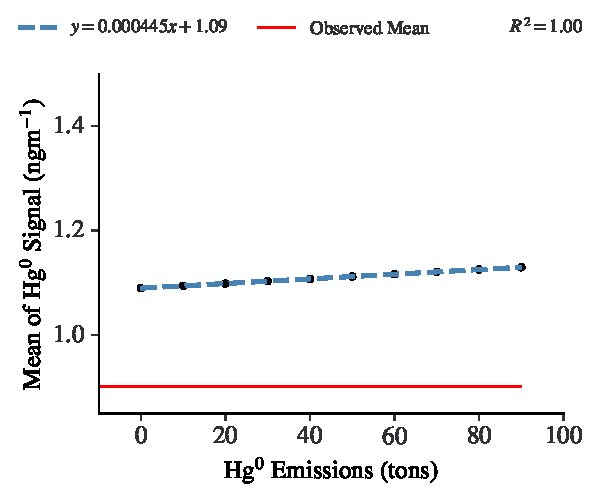
\includegraphics[width = 0.45\linewidth]{templates/figures/individual_site_modifications/mean_Aqp_sigs.pdf}} &
\subfloat[Apurimac]{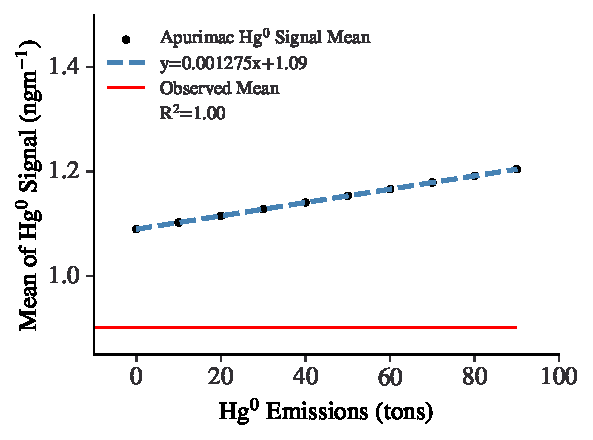
\includegraphics[width = 0.45\linewidth]{templates/figures/individual_site_modifications/mean_Apr_sigs.pdf}}\\
\subfloat[Madre de Dios]{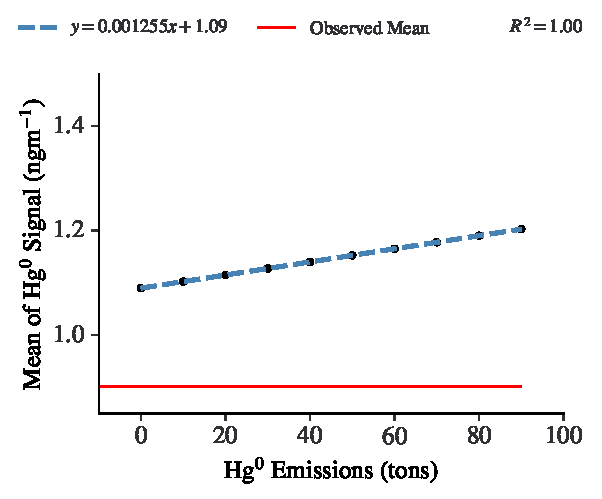
\includegraphics[width = 0.45\linewidth]{templates/figures/individual_site_modifications/mean_Mdd_sigs.pdf}} & \subfloat{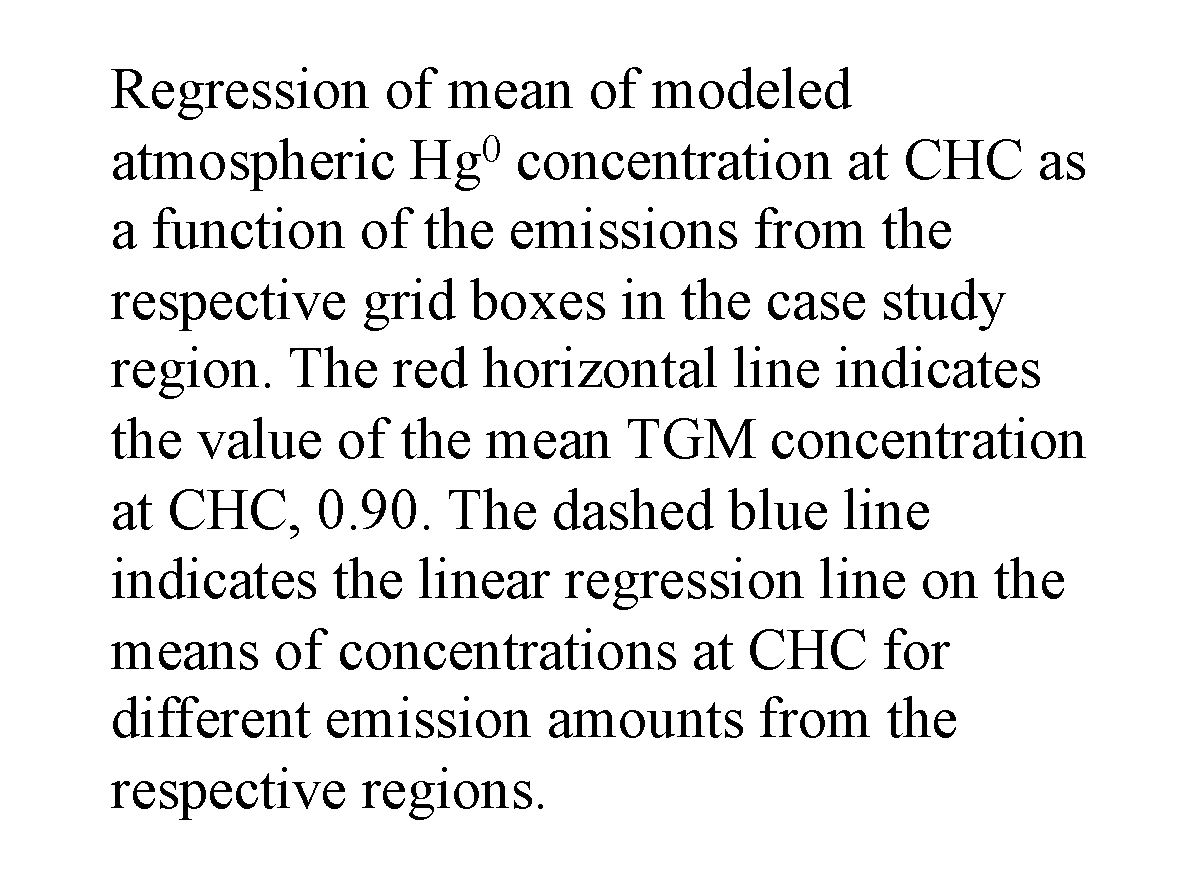
\includegraphics[width = 0.45\linewidth]{templates/figures/individual_site_modifications/mean_caption.pdf}}
\end{tabular}
\caption{ }
\label{fig:mean_of_signals_vs_emissions_per_site}
\end{figure}
\FloatBarrier

% \begin{figure}[H]
%   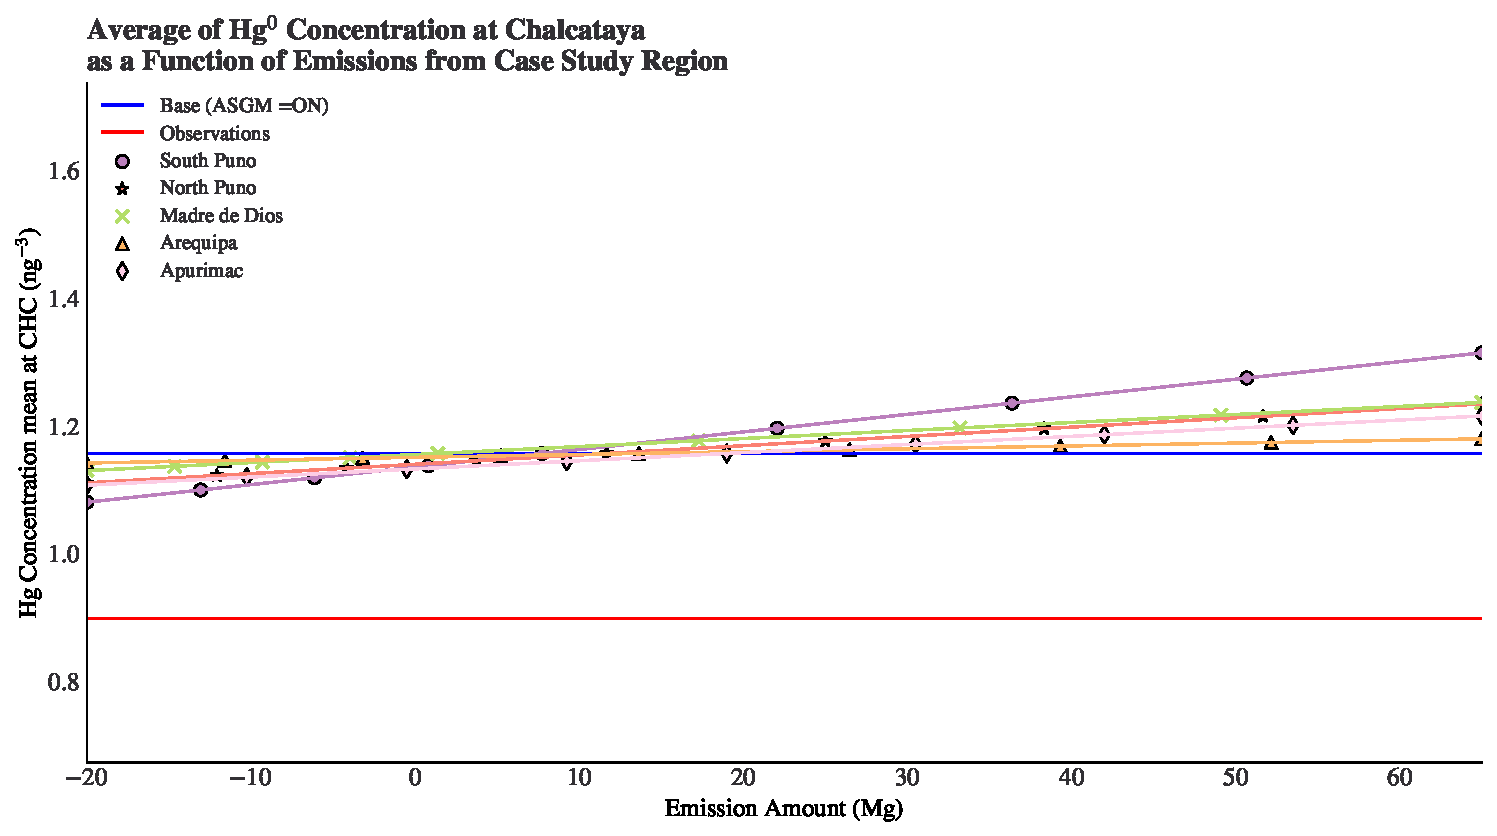
\includegraphics[width=\textwidth]{templates/figures/individual_site_modifications/mean_vs_emissions.pdf}
%   \centering
%   \caption{Modeled average atmospheric \hg concentrations at CHC between 2014/07-2015/07. The red horizontal line indicates the y coordinate observed average TGM concentration of 0.90. The blue horizontal line indicates the average value of the \hg predicted by the \on. The following shapes show the relationships between the concentration at CHC and the emissions from grid boxes in the case study region: South Puno(circles), North Puno (stars), Madre de Dios (green cross), Arequipa (triangle), Apurimac (diamond)  }
%   \label{fig:mean_vs_emissions}
% \end{figure}
% \FloatBarrier
\newpage
\begin{flushleft}
    Contrary to Figure \ref{fig:mean_of_signals_vs_emissions_per_site} where the relationship between the Hg emissions and the mean of \modelc is uniform across all the sites, the relationship between the \iq of \modelc  and the emissions from each grid box in Figure \ref{fig:iqr_vs_emissions_per_site} is not uniform. The plots for the different sites have \rsq values that are different. Even though the \rsq values are different, they are all above 0.85 which means that the regression model given by the equations of the blue dashed line explain the variability of the values of the \iq of \modelc. The values of the \iq for a given amount of Hg emissions from each grid box are compared to the red horizontal line, which indicates the \iq of \obsC, 0.16 as presented in Table \ref{tab:ModelvsObsStats}. 
    %The colored shapes and corresponding lines show the relationships between the \iq of the modeled \hgc at CHC as a function of the emissions from grid boxes in the case study region: South Puno(purple circles connected by the purple line), North Puno (stars connected by the pink line), Madre de Dios (green cross connected by the green line), Arequipa (orange triangles connected by the orange line), Apurimac (peach diamond connected by the peach line).
\end{flushleft}
\begin{flushleft}
     All the lines showing the relationship between the \iq of \modelc and the emissions intersect the red line representing the \iq of \obsC. The Hg emissions value of the point of intersection between the regression line and the red line can be interpreted as what the emissions from the given grid box should be for the \modelc to match the \obsC. The actual values of the emissions can also be calculated using the regression equation given on each plot. These estimates are shown in Table \ref{tab:single_site-change_estimates}, and they provide rough constraints on what the emissions from each grid box would have to be for \modelc to match \obsC.
     
     
\end{flushleft}

% \begin{flushleft}
%     These estimates are the first ever top-down estimates of Hg emissions from ASGM activities. The top-down estimates mostly agree with the bottom-up estimates from Puno
% \end{flushleft}
\begin{figure}[H]
%This could be interpreted to means that the emissions from these grid boxes need to be reduced for \modelc to match \obsC. If the relationship between the \iq and emissions depicted in this Figure were to be taken at face value, the emissions from Madre de Dios would have to be 34.18 tonnes. Moreover, the emissions from North Puno would have to be very close to zero, while those from South Puno would have to be about 4 tonnes, and those from Apurimac would have to be about 6 tonnes.  As bottom-up estimates show, reducing emissions from the Madre de Dios region would not be feasible since emissions from Madre de Dios are higher\cite{agc_reporte_2017}. Thus, the intersection of the lines in Figure \ref{fig:iqr_vs_emissions_per_site} with the line representing the observed \iq should not be taken as an indication that emissions from a single source region can lead to a modeled concentration at CHC that matches the observed \iq. 
\begin{tabular}[H]{cc}
\centering

\subfloat[South Puno]{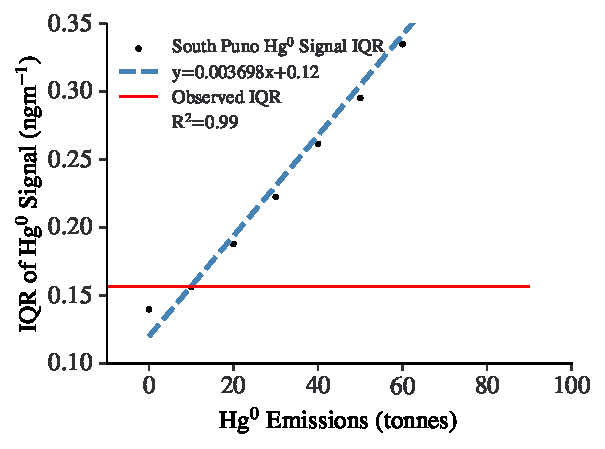
\includegraphics[width = 0.45\linewidth]{templates/figures/individual_site_modifications/iqrSpun_sigs.pdf}} &
\subfloat[North Puno]{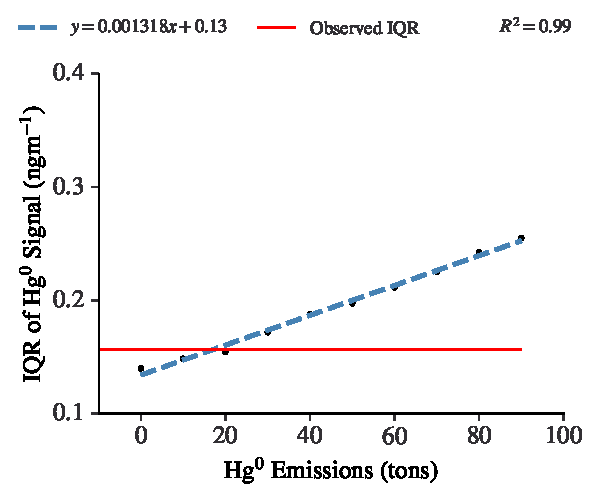
\includegraphics[width = 0.45\linewidth]{templates/figures/individual_site_modifications/iqrNpun_sigs.pdf}}\\
\subfloat[Arequipa]{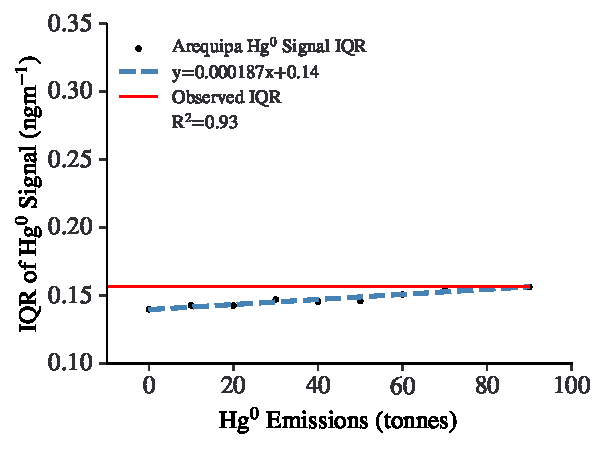
\includegraphics[width = 0.45\linewidth]{templates/figures/individual_site_modifications/iqrAqp_sigs.pdf}} &
\subfloat[Apurimac]{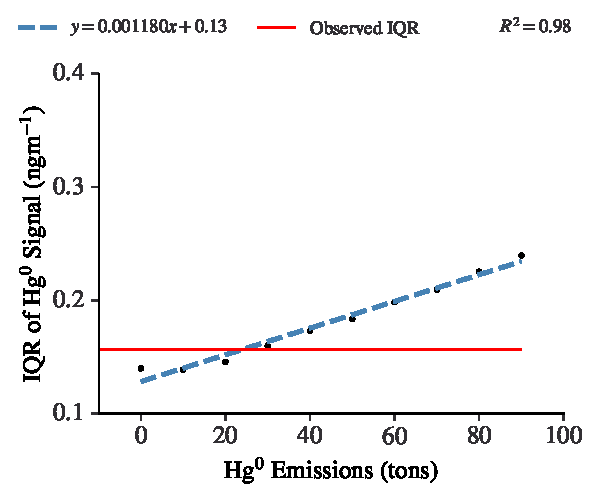
\includegraphics[width = 0.45\linewidth]{templates/figures/individual_site_modifications/iqrApr_sigs.pdf}}\\
\subfloat[Madre de Dios]{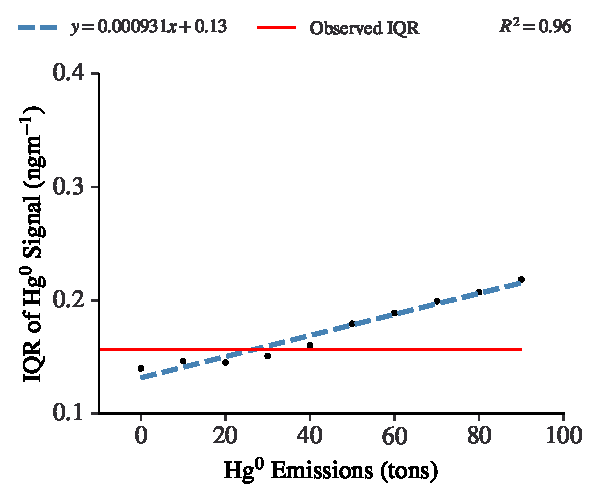
\includegraphics[width = 0.45\linewidth]{templates/figures/individual_site_modifications/iqrMdd_sigs.pdf}} & \subfloat{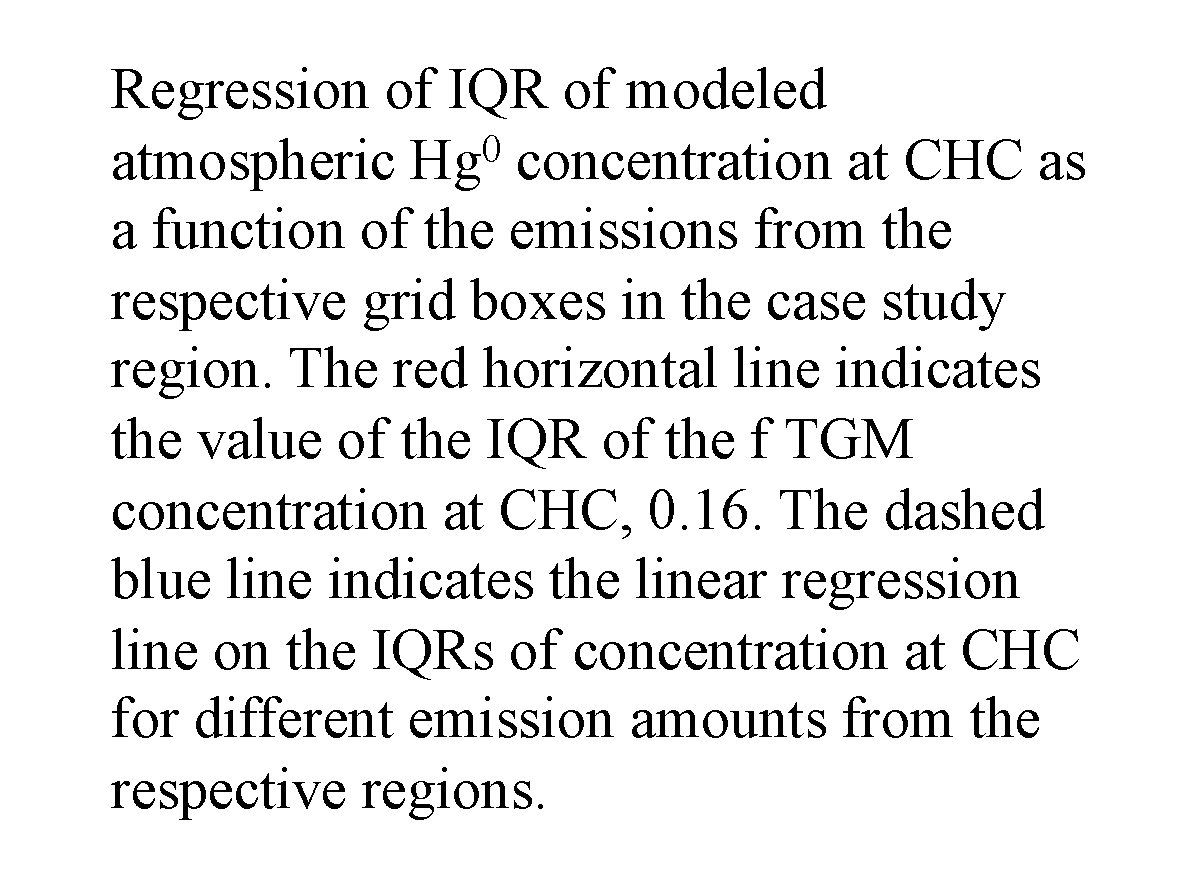
\includegraphics[width = 0.45\linewidth]{templates/figures/individual_site_modifications/iqrcaption.pdf}}
\end{tabular}
\caption{}
\label{fig:iqr_vs_emissions_per_site}
\end{figure}
\FloatBarrier
% \begin{figure}[H]
%   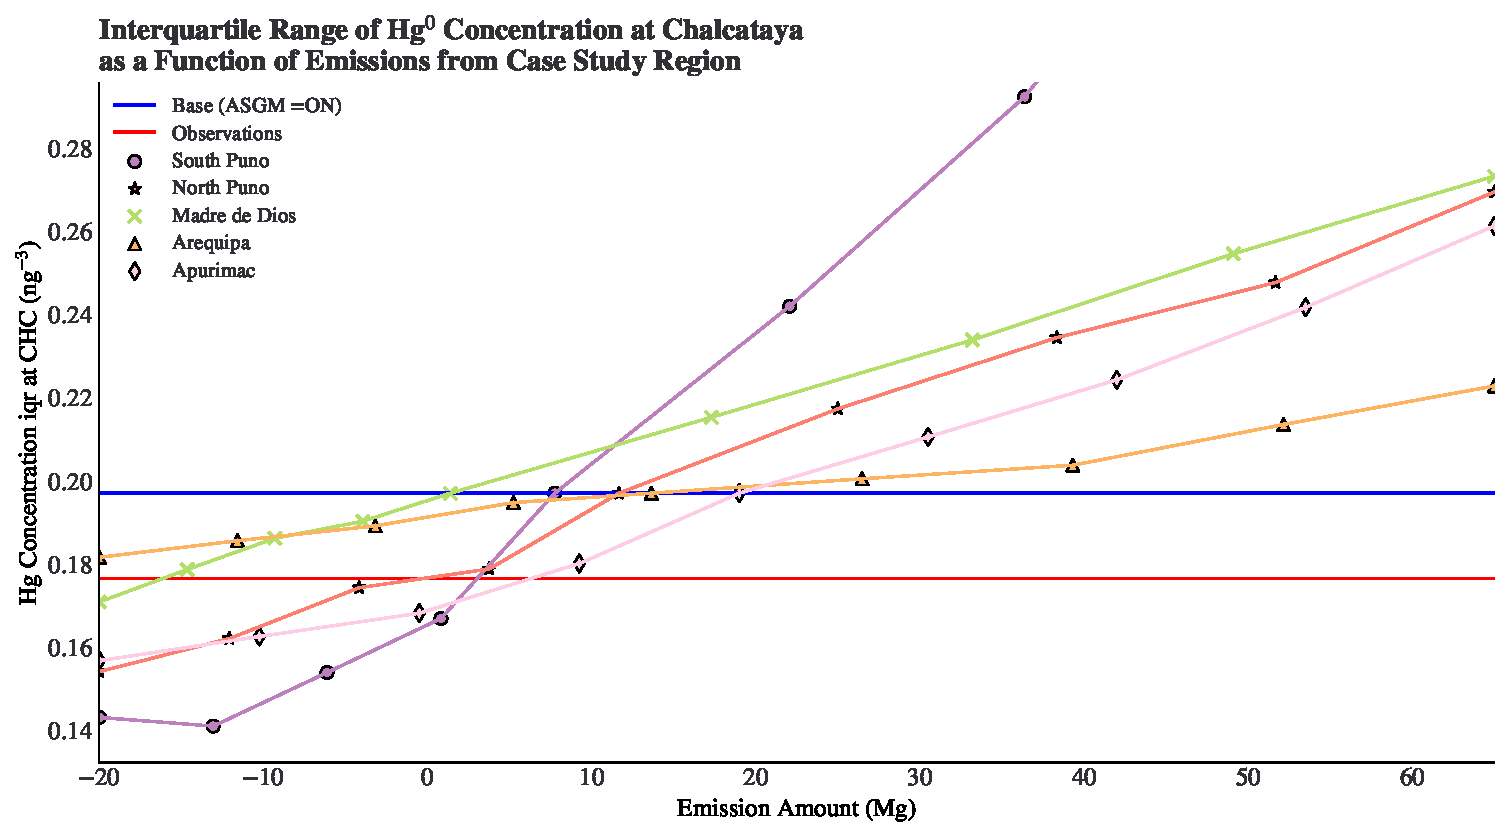
\includegraphics[width=\textwidth]{templates/figures/individual_site_modifications/iqr_vs_emissions.pdf}
%   \centering
%   \caption{ Plot of IQR of \obsC and \modelc as a function of emissions from the case study region. The red horizontal line indicates the observed TGM concentration IQR(0.18). The blue horizontal line indicates the \on predicted \hg IQR. The following shapes show the relationships between the modeled \hg concentration signal IQR at CHC as a function of the emissions from grid boxes in the case study region: South Puno (purple line with circle markers), North Puno (congo pink line with star markers), Madre de Dios (green line with cross markers), Arequipa (orange line with triangle markers), and Apurimac (classic rose line with diamond markers  }
%   \label{fig:iqr_vs_emissions}
% \end{figure}
% \FloatBarrier
\newpage
\begin{flushleft}
     
     Unlike the relationships evident in Figures \ref{fig:mean_of_signals_vs_emissions_per_site} and \ref{fig:iqr_vs_emissions_per_site}, where the relationship between the emissions and the mean or \iq of \modelc is positive, the relationship between the emissions and correlation of \modelc and \obsC shown in Figure \ref{fig:corr_vs_emissions} is negative. The red horizontal line indicates the Pearson correlation between \obsC and the \on. The dashed blue line shows the regression line of the correlation between \modelc and \obsC as emissions from each grid box increase. These plots show that it is impossible to improve the Pearson correlation between \modelc and \obsC by changing the emissions.
     
     %The different lines show the correlation between \modelc and \obsC as a function of the emissions from each of the regions: South Puno (purple line with circle markers), North Puno (congo pink line with star markers), Madre de Dios (green line with cross markers), Arequipa (orange line with triangle markers), and Apurimac (classic rose line with diamond markers) The correlation decreases as the emissions from the South Puno, Arequipa, and Apurimac grid boxes increase. 
     
     %These relationships show that changing the emissions from one grid box in the\gc model may not be a reliable way to improve the model's prediction of the observed concentrations, especially because ASGM is no. 

\end{flushleft}


% \begin{figure}[H]
%   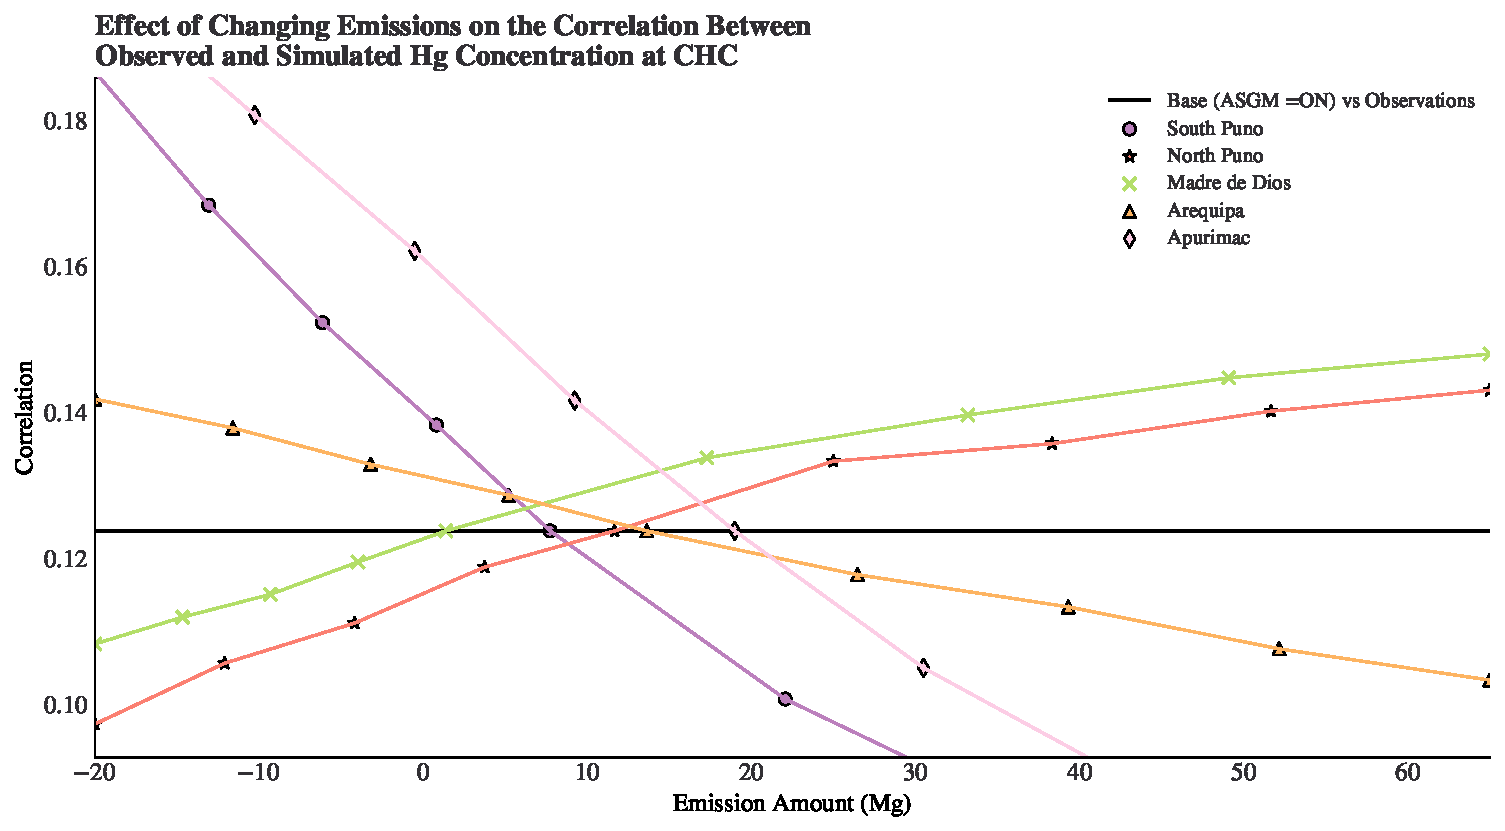
\includegraphics[width=\textwidth]{templates/figures/individual_site_modifications/correlation_vs_emissions.pdf}
%   \centering
%   \caption{Correlation between \obsC and \modelc as a function of emissions from grid boxes associated with the case study region. The black horizontal line indicates the Pearson correlation between \obsC and the \on. The different lines show the correlation between \modelc and \obsC as a function of the emissions from each of the regions: South Puno (purple line with circle markers), North Puno (congo pink line with star markers), Madre de Dios (green line with cross markers), Arequipa (orange line with triangle markers), and Apurimac (classic rose line with diamond markers)}
%   \label{fig:correlation_vs_emissions}
% \end{figure}
% \FloatBarrier
\begin{figure}[H]
\begin{tabular}[H]{cc}
\centering

\subfloat[South Puno]{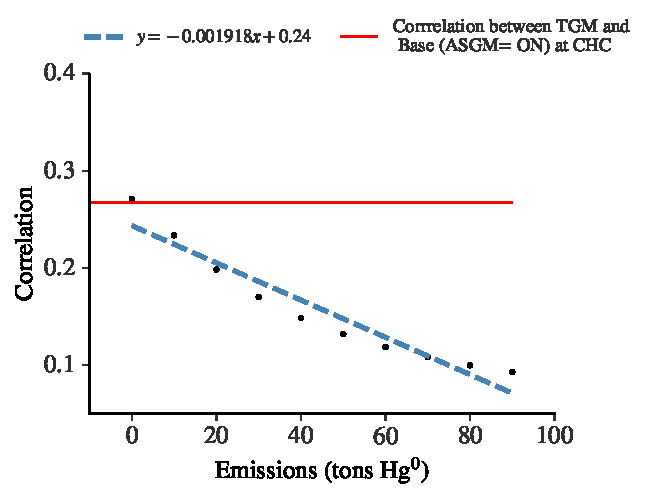
\includegraphics[width = 0.45\linewidth]{templates/figures/individual_site_modifications/corr_Spun_sigs.pdf}} &
\subfloat[North Puno]{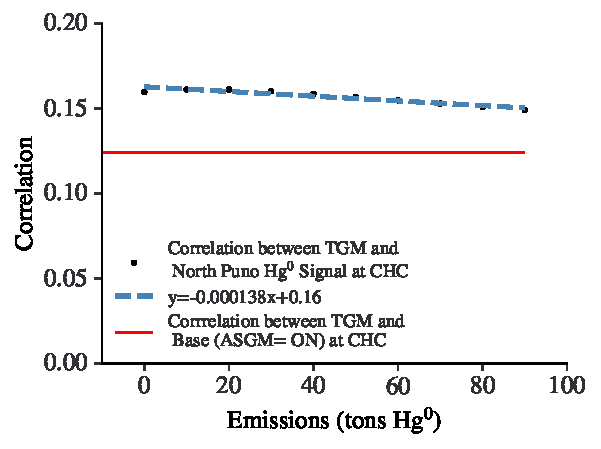
\includegraphics[width = 0.45\linewidth]{templates/figures/individual_site_modifications/corr_Npun_sigs.pdf}}\\
\subfloat[Arequipa]{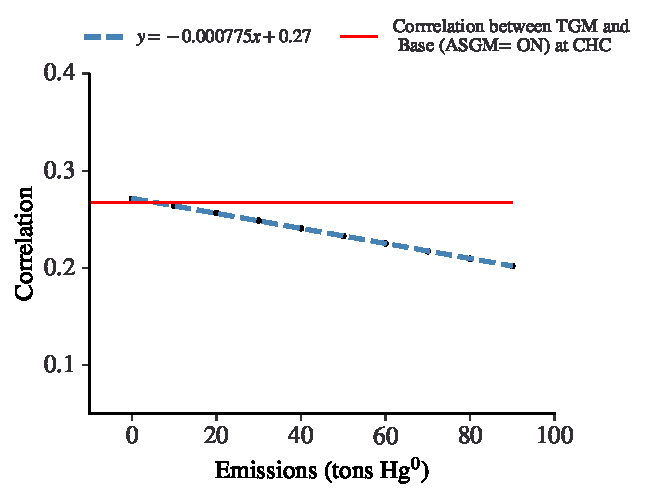
\includegraphics[width = 0.45\linewidth]{templates/figures/individual_site_modifications/corr_Aqp_sigs.pdf}} &
\subfloat[Apurimac]{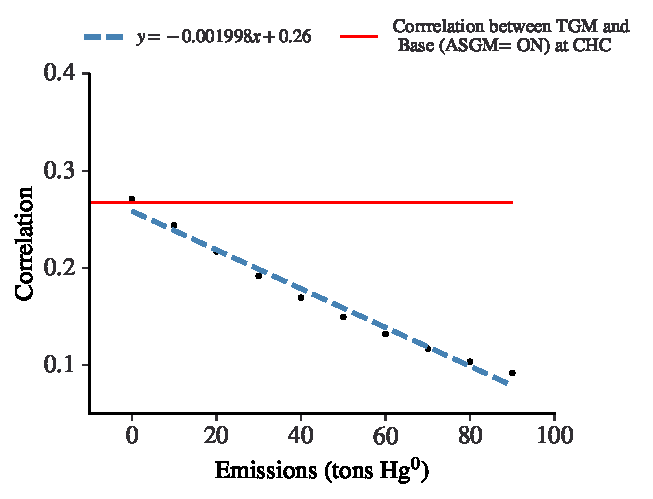
\includegraphics[width = 0.45\linewidth]{templates/figures/individual_site_modifications/corr_Apr_sigs.pdf}}\\
\subfloat[Madre de Dios]{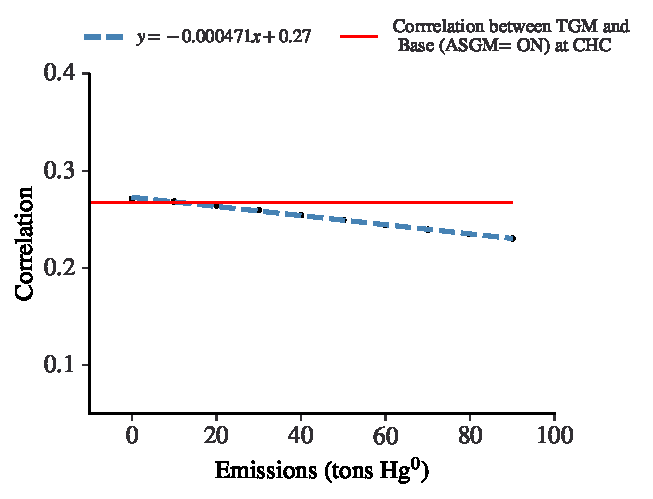
\includegraphics[width = 0.45\linewidth]{templates/figures/individual_site_modifications/corr_Mdd_sigs.pdf}} & \subfloat{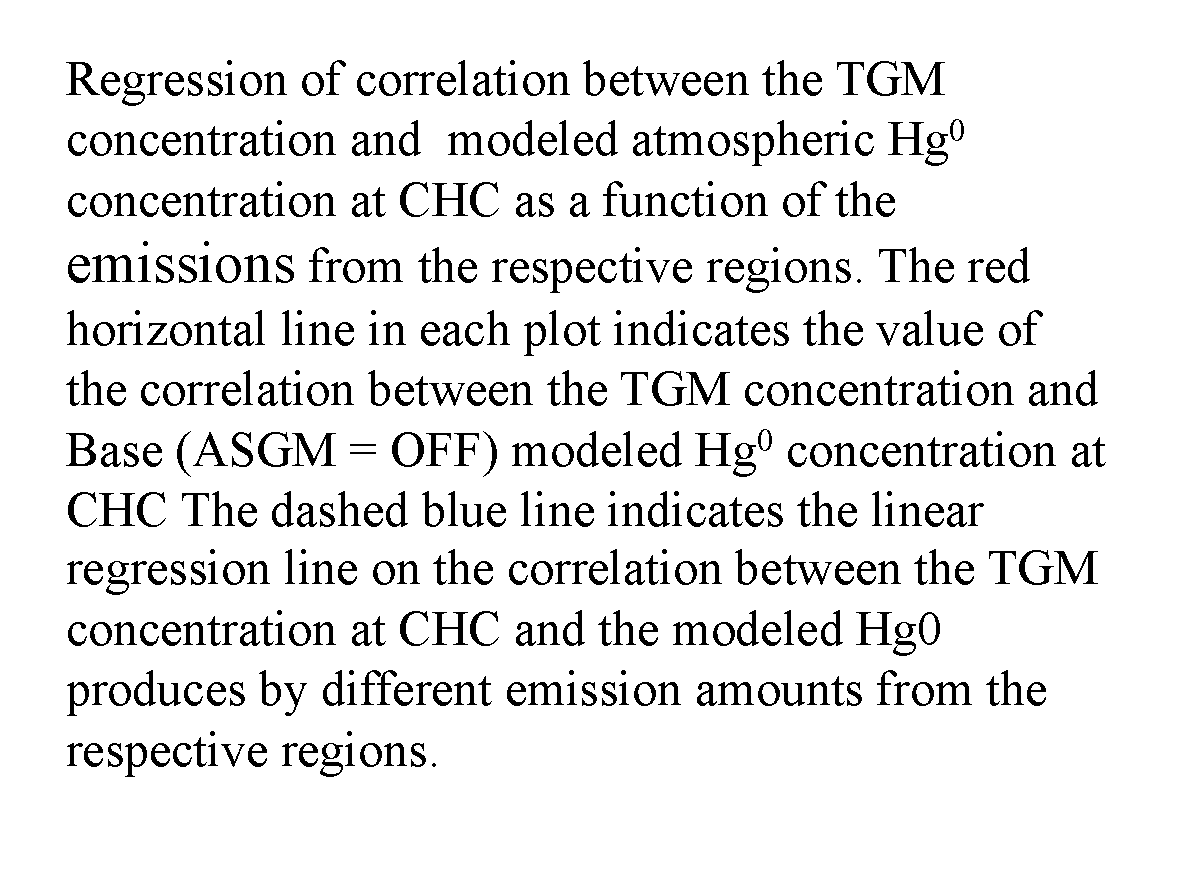
\includegraphics[width = 0.45\linewidth]{templates/figures/individual_site_modifications/corr_caption.pdf}}
\end{tabular}
\caption{ }
\label{fig:corr_vs_emissions}
\end{figure}
\FloatBarrier
\newpage
\begin{table}[H]
\caption{Table showing the emission estimates for each of the grid boxes in the case study region when the \iq is used as the metric to compare \modelc to \obsC after modifying emissions from one site and when the \nft is used}
    \label{tab:single_site-change_estimates}
\begin{tabular}{lcc}

\textbf{Region}        & \textbf{Emission Estimate }        &  \textbf{Emission Estimate }\\
                        &  \iq (tonnes)       &   \nft (tonnes) \\
\hline
Madre de Dios          & $26.82$                                    & $78.10$ \\

North Puno             & $17.16$                                   & $24.87$  \\
        
South Puno             & $9.93$                                    & $59.46$   \\

Apurimac               & $24.08$                                   & $62.86$  \\

Arequipa               & $90.77$                                   & $178.45$  \\


\hline
\end{tabular}
\centering
\end{table}
\begin{flushleft}
     This section has shown the effect of changing Hg emissions from individual grid boxes on the modeled \hgc at a distant active monitoring site like CHC. The \iq and \nft produced some estimates of the \hg emissions from the different regions. However, the range of these estimates is not within the estimates discussed in  section 3.3.1. These estimates were more informative about the potential constraints on the emissions from the region. The following section presents the emission estimates generated using the MCMC to investigate the effect of changing emissions from multiple sites instead of changing the emissions from one site as discussed in this section.  
     
     %Other processes, such as vegetation uptake, have been shown to impact the amount of Hg in the atmosphere, and Feinberg et al 2022 showed that this version of \gc had a poor representation of vegetation uptake\cite{feinberg_evaluating_2022}.  Furthermore, comparing the Peru national inventory of emissions developed by the AGC\cite{agc_reporte_2017} and the global inventory in the GMA 2018\cite{steenhuisen_development_2019,united_nations_environment_programme_technical_2019} as we did in section 3.3.1 shows that there are numerous mismatches between the actual emissions and the emissions used by \gc to simulate the \hgc in the atmosphere.

   
 
\end{flushleft}

\subsection{Estimating Emissions with Markov Chain Monte Carlo}
The MCMC approach produced \hg emissions estimates within the ranges of estimates produced by the bottom-up inventories when the \nft was used to compare \obsC to \modelc. Figure \ref{fig:MCMC_estimates95th} show's the distributions of the estimates produced by the MCMC approach. The \hg emission estimates when the \nft is used as the metric to compare \modelc, and \obsC is shown by the box and whisker plots. The horizontal lines representing the emission estimates from the bottom-up inventories are traced over the box plots. The solid horizontal lines represent the emission estimates from the GMA 2018 inventory \cite{united_nations_environment_programme_technical_2019,steenhuisen_development_2019} and the dashed lines represent the emission estimates from the bottom-up inventory published by the Artisanal Gold Counsel\cite{agc_reporte_2017}. The estimated values and ranges of emissions are detailed in Table \ref{tab:MCMC_estimates}. 
\begin{figure}[H]
  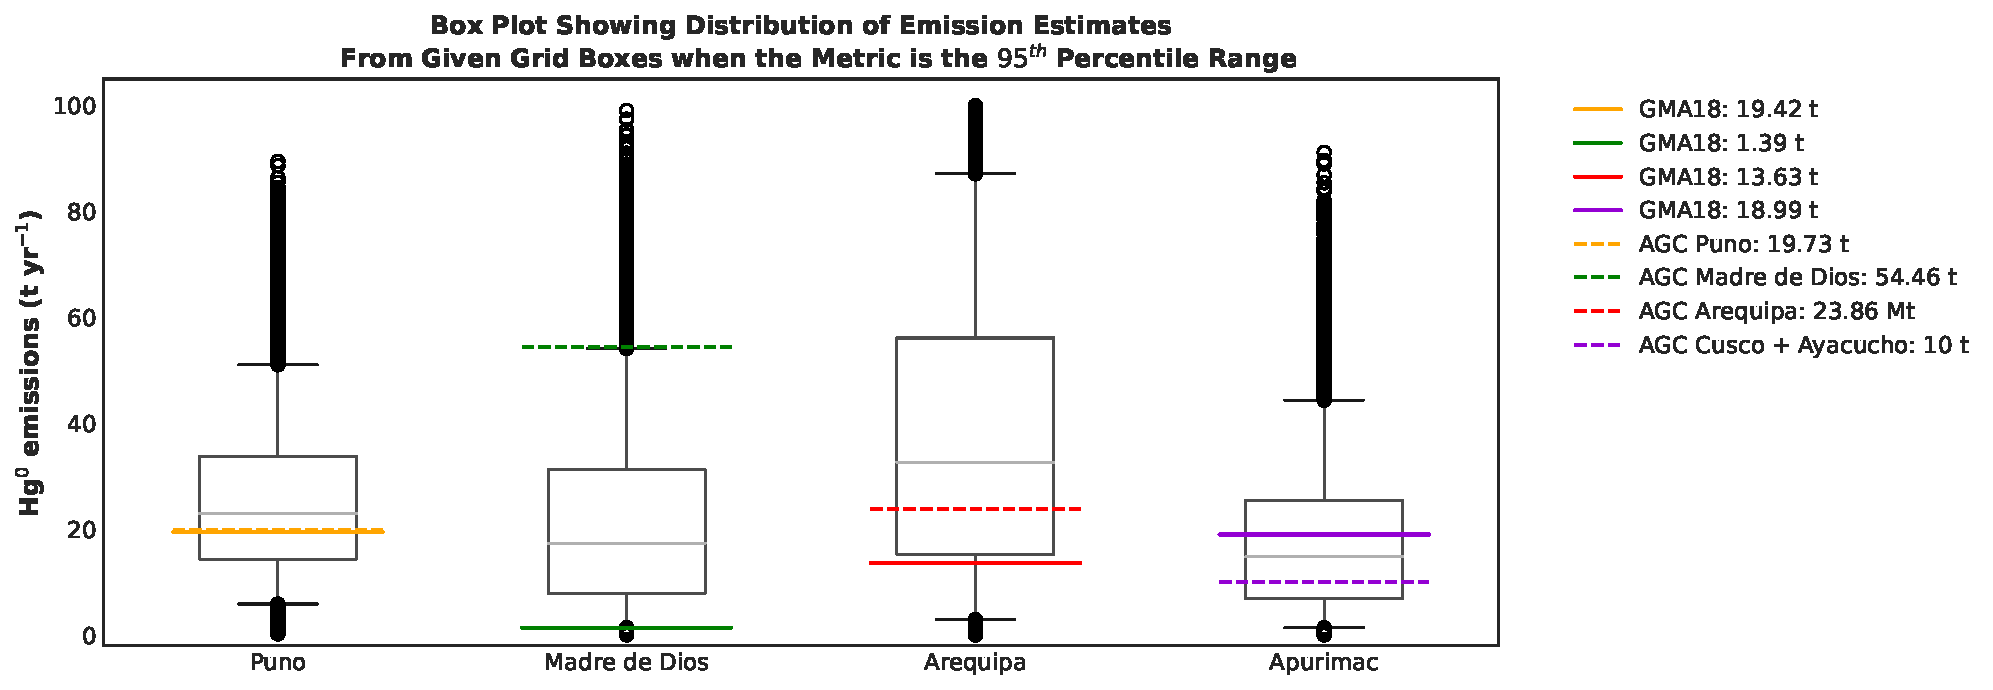
\includegraphics[width=\textwidth]{templates/figures/MCMC/MCMCMCMC_Estimates95th.pdf}
  \centering
  \caption{Emission Estimates when the $95^{th}$ percentile range is used as the metric to compare the model outputs to observations. The horizontal lines representing the emission estimates from the bottom-up inventories are traced over the box plots. The solid horizontal lines represent the emission estimates from the GMA 2018 inventory \cite{united_nations_environment_programme_technical_2019,steenhuisen_development_2019} and the dashed lines represent the emission estimates from the bottom-up inventory published by the Artisanal Gold Counsel\cite{agc_reporte_2017}.}
  \label{fig:MCMC_estimates95th}
\end{figure}
\FloatBarrier
% % \renewcommand{\arraystretch}{2}
% \begin{flushleft}
%      The mean was the worst metric to use in the MCMC to reproduce the GMA 2018 emissions estimates, while the \nft reproduced the GMA 2018 emissions estimates with the least absolute error, followed by the \iq. This further corroborated the earlier finding that the mean was not a reliable metric, in this case, to compare the observed Hg concentration in the atmosphere to the modeled \hg concentrations.
% \end{flushleft}

%      Figure \ref{fig:MCMC_emetrics} compares the absolute error of different metrics when used in the MCMC to generate estimates of the emissions from different departments in Peru. The absolute error is a function of the type of metric used. The plus signs show the absolute error in reproducing emissions from the case study region(Puno (blue), Madre de Dios (orange), Arequipa (green), and Apurimac (red)) for each metric.

% \begin{figure}[H]
%   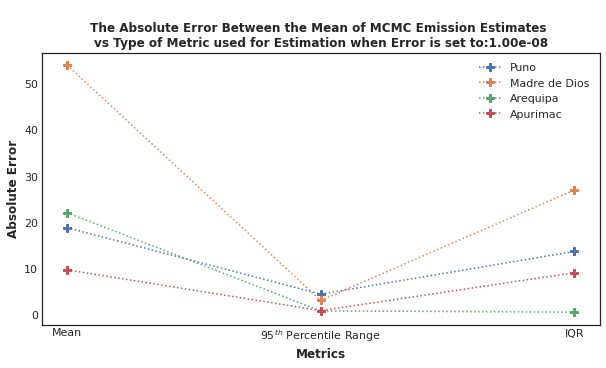
\includegraphics[width=\textwidth]{templates/figures/MCMC/comparison of matrics.png}
%   \centering
%   \caption{Comparison of the absolute error of different metrics when used in the MCMC to generate estimates of the emissions from different grid boxes in the case study region. The Absolute error is a function of the type of metric used. The plus signs show the absolute error in reproducing emissions from the case study region(Puno (blue), Madre de Dios (orange), Arequipa (green), and Apurimac (red)) for each metric.  }
%   \label{fig:MCMC_emetrics}
% \end{figure}
% \FloatBarrier
\begin{flushleft}
    These estimates are the first ever top-down estimates of Hg emissions from ASGM activities. It is critical to note that the ranges of the estimates are huge. Therefore, these results may be improved if more data from monitoring sites were available to constrain the emissions. 
\end{flushleft}    
\begin{table}[H]
\caption{Table showing the emission estimates for each of the grid boxes in the case study region when the $95^{th}$ percentile range is used as the metric to compare the model outputs to observations}
    \label{tab:MCMC_estimates}
\begin{tabular}{lcc}

\textbf{Region}        & \textbf{Emission Estimate (Mg)}  &     \textbf{Range of Estimate (Mg)}                      \\
\hline
Madre de Dios          & $21$                               & $1.36 - 54.12$\\

Apurimac               & $17$                               & $1.36 - 44.37$\\

Arequipa               & $37$                               & $2.88 - 87.14$\\

Puno                    & $25$                              & $5.85 - 51.05$\\
\hline
Total                  & $101.23$                            &  $11.45 - 236.69$ \\
\hline
\end{tabular}
\centering
\end{table}

\begin{flushleft}
 % I argued that poor parameterization of dry deposition in \gcs version 12.8.1 might be one of the reasons for this poor performance of the model in reproducing the mean of \obsC. Moreover, this phenomenon was investigated and addressed for future \gc versions in Feinberg et al (2022). I also hypothesized that the model poorly predicted Hg concentrations in the atmosphere because of faults in the emission estimates used in the model. 
  We produced top-down estimates of the corresponding emissions for four Peruvian departments in the case study region. The estimated emissions and the ranges are shown in Table \ref{tab:MCMC_estimates} resulting in 101.23 tonnes of emissions from Peru per year, ranging from 11.45 tonnes to 236.69 tonnes. This is a wide range, but it's a confidence interval based on the data and model uncertainty discussed so far. The proof of concept I developed shows that even with a minimal data set and an uncertain model, we can calculate top-down estimates of ASGM \hg emissions. Improved parameterization of vegetation uptake will narrow the vast uncertainty ranges in the emission estimates produced by this approach and improve confidence in the \hg emission estimates. Such model improvements are discussed in Feinberg et al.(2022)\cite{feinberg_evaluating_2022} and may enable the use of the mean as a metric for producing the \hg emission estimates, which we could not not use in this analysis. Additional data is another essential source of improvement, particularly time series data rather than annual averages as I have shown by using different time periods from \obsC dataset. Moreover, these results demonstrate that for non-point sources, such as ASGM, where the variability over time is somewhat unpredictable, extreme values provide vital information for source quantification. The analysis in this chapter focused on a region in Peru, where ASGM dominates to use top-down techniques for quantifying ASGM Hg emissions. Implementing this approach will be challenging in areas where ASGM occurs concurrently with many point sources, such as Southeast Asia where biomass burning and coal combustion. For Hg monitoring sites in mountainous regions such as CHC, the global scale resolution of GEOS-Chem is not particularly suitable. Therefore, future work may extend this method and this proof of concept using finer resolutions with a regional focus.
\end{flushleft}

% \begin{figure}[H]
%   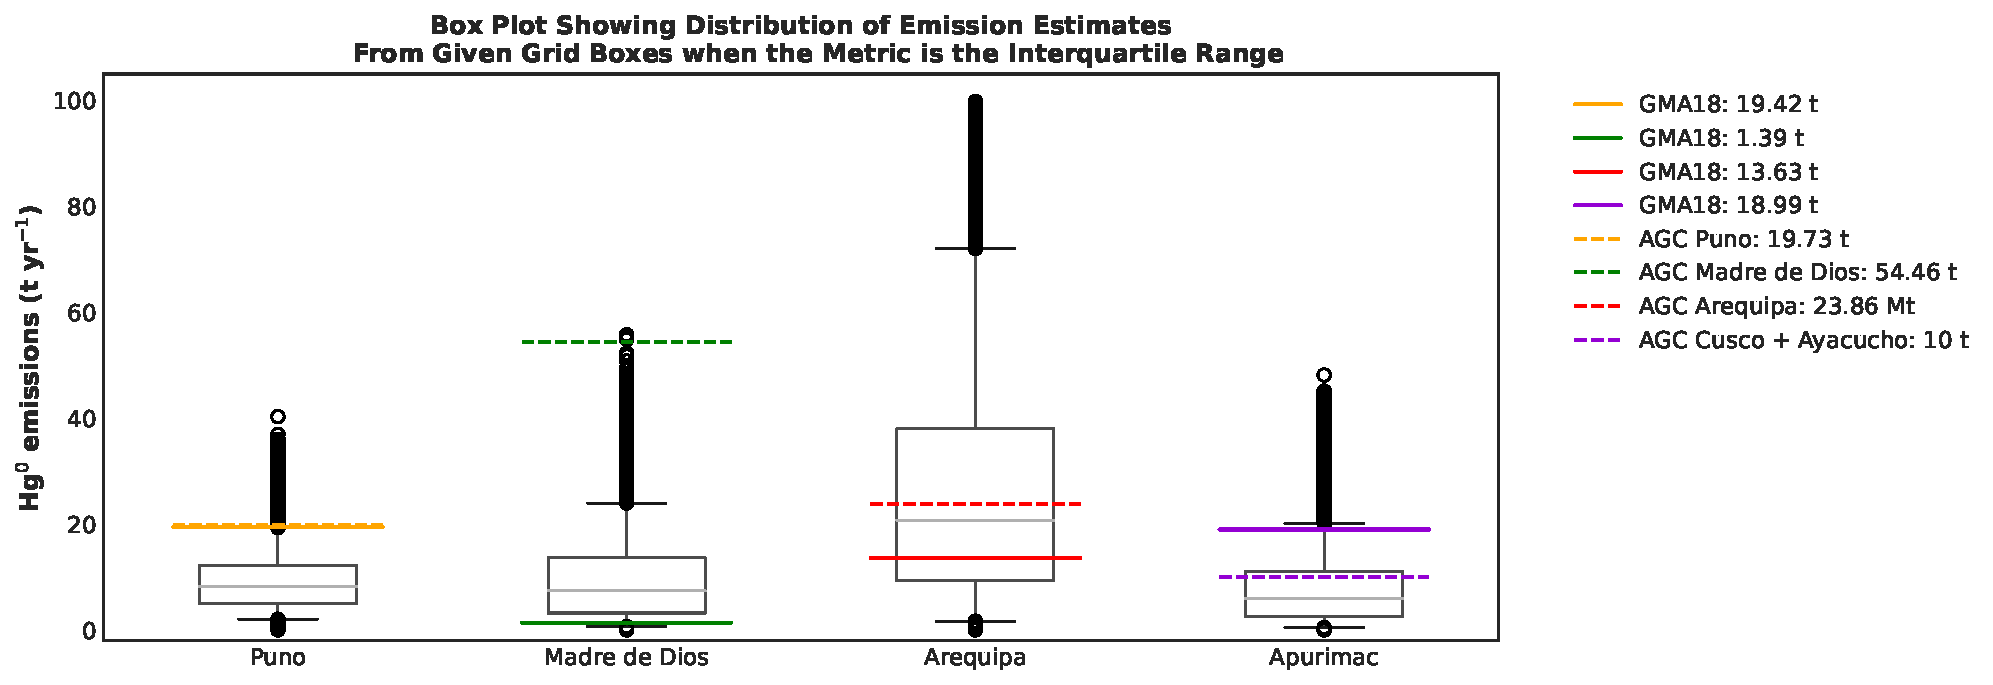
\includegraphics[width=\textwidth]{templates/figures/MCMC/MCMCMCMC_Estimatesiqr.pdf}
%   \centering
%   \caption{Emission Estimates when the \iq is used as the metric to compare the model outputs to observations. The horizontal lines representing the emission estimates from the bottom-up inventories are traced over the box plots. The solid horizontal lines represent the emission estimates from the GMA 2018 inventory \cite{united_nations_environment_programme_technical_2019,steenhuisen_development_2019} and the dashed lines represent the emission estimates from the bottom-up inventory published by the Artisanal Gold Counsel\cite{agc_reporte_2017}.}
%   \label{fig:MCMC_estimates95}
% \end{figure}
% \FloatBarrier

\section{Conclusion}
\begin{flushleft}
In this study, I demonstrate how top-down estimates of Hg emissions from ASGM activities can be generated using a CTM and time series monitoring data. Limited data sources and uncertain models prevented precise calculations, but the emissions were within the ranges estimated by the GMA 2018\cite{steenhuisen_development_2019,united_nations_environment_programme_technical_2019} and the Artisanal Gold Council\cite{agc_reporte_2017}. By defining vegetation uptake better, the model improvements discussed in Feinberg et al. (2022) will improve this approach and potentially increase the utility of mean concentrations as a viable metric to use in the analysis\cite{feinberg_evaluating_2022}. Additionally, more time series data will enhance the accuracy and credibility of the model's estimates. Given future work and interest in applying this method in other regions, I noted that this approach was applied to a case study region in Latin America, where ASGM is the dominant source. It may be challenging to extend this approach to areas where ASGM Hg emissions occur in tandem with other emission sources.
 
\end{flushleft}


\chapter{Policy Recommendations and Conclusions}
\begin{flushleft}
    

This chapter aims to provide policy recommendations about using atmospheric models and monitoring to provide information about ASGM Hg emissions to the atmosphere. The policy recommendations will build upon the information discussed in the earlier chapters of the thesis. Chapter one discussed the nature of ASGM activities and their contribution to the global Hg budget. Existing challenges regarding knowledge of ASGM Hg emissions were discussed. For instance, the huge uncertainties in ASGM Hg emission estimates and the discrepancies between national and global estimates were highlighted \cite{united_nations_environment_programme_technical_2019,agc_reporte_2017}. This thesis was partly motivated by the lack of atmospheric monitoring in ASGM regions and the absence of modeling studies evaluating Hg emissions from regions with high ASGM emissions.
Moreover, Chapters 2 and 3 showed how different Hg atmospheric concentrations data sources could be leveraged and integrated with the GEOS-Chem CTM results to investigate ASGM Hg pollution. Chapter 2 compared the temporal and spatial characteristics of observed and modeled atmospheric Hg concentrations. Passive Air Sampling of atmospheric Hg concentrations was shown to provide helpful information about the distribution of Hg concentrations across Latin America. Additionally, it was discussed that a network of PAS provides high-quality data while being accessible and affordable to deploy\cite{quant_measuring_2021}.  On the other hand, active sampling techniques conducted by the GMOS Network were found to provide valuable time series data about the atmospheric Hg concentrations. The time series data from these networks provide more metrics to evaluate ASGM emissions and enable the evaluation of intra-year variations of Hg concentrations in the atmosphere, which may help improve understanding of the seasonality in ASGM activities. For instance, in Chapter 3, I showed that the IQR and the 95th percentile range could be used to provide a reasonable estimate of the Hg emissions from Peru. 
\end{flushleft}
\begin{flushleft}
Section \ref{nap_gma18_differences} compares the GMA 2018 estimates to the estimates that countries have provided in their NAPs to highlight the value that atmospheric monitoring the modeling would add to the policy-making process. Moreover, section \ref{motreal_protocol_comparison} uses the Montreal Protocol as an example to discuss the possibilities provided by combining atmospheric monitoring and modeling to inform actions by parties as well as evaluate the effectiveness of an international treaty about a hazardous substance. I discuss the point that atmospheric monitoring and modeling provides valuable information but may be politically controversial depending on the expectation of parties and the type of penalties imposed on violators of international emission regulation laws. Next, section 4.2 discusses recommendations for governments by highlighting the fact that governments should prioritize atmospheric monitoring. Moreover, PAS technologies may be the low-hanging fruits that governments roll out as part of the implementation plan since they are affordable and require less skilled technical know-how to set up and maintain \cite{quant_measuring_2021}. Furthermore, I encourage countries to pursue regional active monitoring  by showing that this thesis provides insight into the possibility of understanding ASGM Hg emissions from one high-frequency and quality data monitoring site. Finally, the recommendations are summarised in the conclusion. 
\end{flushleft}

\section{Discrepancies Between Global and National ASGM Mercury Estimates}\label{nap_gma18_differences}

According to Evers et al.(2016), country-specific actions under Article 7 of the MC will differ from country to country, and this variability poses a challenge to assessing the MC's effectiveness. Additionally, they argue that changes in the overall use of Hg in the global ASGM sector can be informed by progress in individual countries. They suggest a compilation, visualization, and mapping of the respective data to track this progress across ASGM countries.  The value added by baseline estimates of emissions to policy making is also recognized in the MC's paragraph 3 of Article 7, which stipulates that each party that notifies the secretariat that (ASGM) and processing in its territory is more than insignificant shall develop and implement a national action plan (NAP) per annex C to the MC. In addition, annex C (d) states that the NAP shall include baseline estimates of the quantities of Hg used and the practices employed in ASGM and processing. As of this writing, 18 countries have submitted their respective NAPs. The estimates of how much Hg is used in their territories are shown in Figure\ref{fig:global-hg-emission-estimates_vs_nap_estimates}, which is a bar chart comparing the estimates of annual average Hg emissions predicted in the GMA 2018 inventory in light blue vs. annual average Hg emissions baseline estimates (shown in dark blue) that were reported by the respective countries in their NAPs \cite{united_nations_environment_programme_technical_2019}.

\begin{figure}[H]
  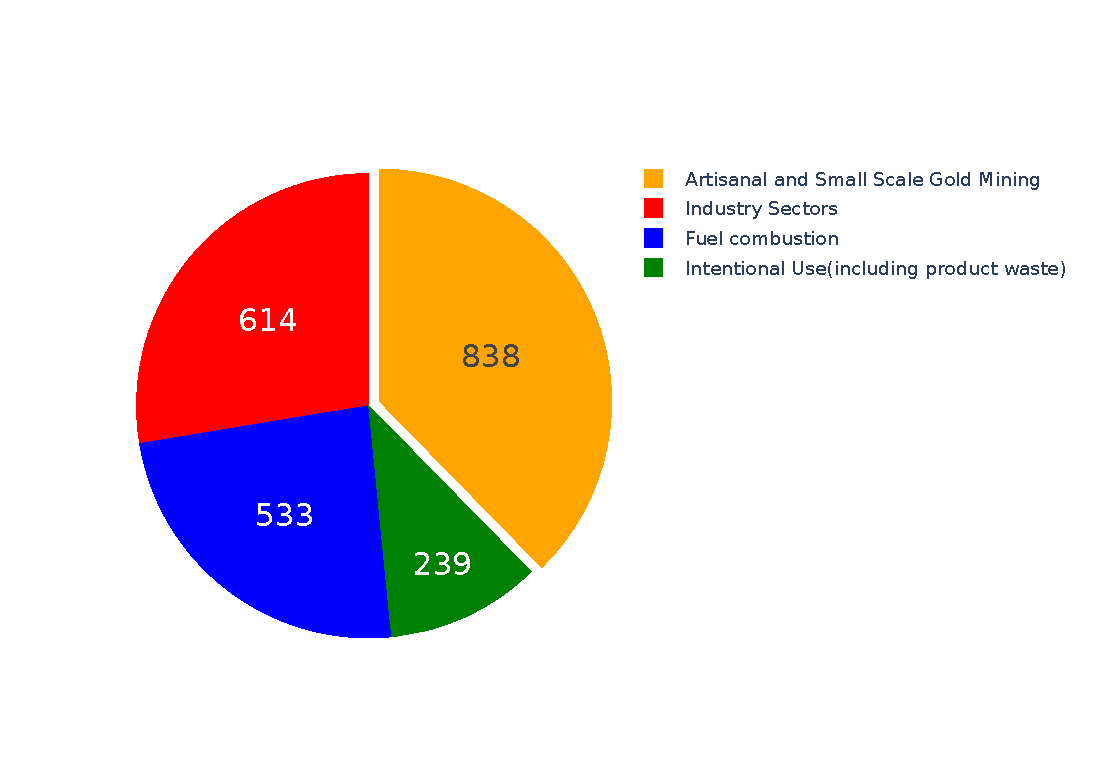
\includegraphics[width=\textwidth]{templates/figures/07-24-22_global-hg-emission-estimates_vs_nap_estimates.pdf}
  \centering
  \caption{Bar chart comparing the estimates of annual average Hg emissions predicted in the GMA 2018 inventory in light blue vs. annual average Hg emissions baseline estimates (shown in dark blue) that were reported by the respective countries in their NAPs \cite{united_nations_environment_programme_technical_2019} }
  \label{fig:global-hg-emission-estimates_vs_nap_estimates}
\end{figure}
\FloatBarrier
\begin{flushleft}
 In Figure \ref{fig:global-hg-emission-estimates_vs_nap_estimates}, it is evident that the difference between the global estimates and the NAP estimates is vast for some countries. While the baseline estimates of Hg use in ASGM as reported in the NAPs and global inventories are critical, data from monitoring networks combined with atmospheric models provide additional tools to evaluate the changes in Hg in the atmosphere. The differences in the estimates do not necessarily indicate emission increases, but they reflect the uncertainties in the global emission estimates. 
\end{flushleft} 

\section{Informing the Use of Atmospheric Modeling for Quantifying ASGM Emissions in the Minamata Convention through Experiences from the Montreal Protocol} \label{motreal_protocol_comparison}

\begin{flushleft}
Monitoring atmospheric concentrations of pollutants of interest and using atmospheric models to understand the data has been critical in evaluating global conventions such as the Montreal Protocol. For instance, Rigby et al. 2019 showed how vital the combination of atmospheric monitoring networks and modeling is when they quantified the amount of an observed increase in CFC-11 and identified where the source was located\cite{rigby_increase_2019}. They used high-frequency atmospheric observations from Gosan, South Korea, and Hateruma, Japan, and global monitoring data and atmospheric CTM simulations to investigate regional CFC-11 emissions from eastern Asia.  
\end{flushleft}
\begin{flushleft}
    The above example about the Montreal protocol showcases the multiple benefits of atmospheric monitoring and modeling. For instance, Rigby et al.\cite{rigby_increase_2019}  showed that emissions from eastern mainland China were 7.0 ± 3.0 (±1 standard deviation) gigagrams per year higher in 2014–2017 than in 2008–2012 and that the increase in emissions arose primarily around the northeastern provinces of Shandong and Hebei\cite{rigby_increase_2019}. This kind of precision of emission estimates and the approximate location of their sources would be beneficial for evaluating the effectiveness of MC efforts aimed at reducing Hg emissions. Policymakers would value such information because it would give them precise data about the amounts of emissions and where they should look for the sources. However, it is uncertain if this level of precision could be achieved for an emission source like ASGM, given that it is not a point source.
    
    Another critical aspect of the information provided by the approach discussed in this thesis is the ability to determine areas that have a low likelihood of being sources of increase in emissions. This benefit was also demonstrated  by Rigby et al. (2019)  in that they could conclude that there was no evidence for a significant rise in CFC-11 emissions from any other eastern Asian countries or other regions of the world where there are available data for the detection of regional emissions.
\end{flushleft}

\begin{flushleft}
A look at China's response to scientific information about its increased CFC emissions in the Montreal Protocol example above may provide insight into possible answers by parties when they are notified about emission violations within their territory. China questioned the conclusions of the scientific study noting significant uncertainty. However, they also acknowledged the importance of atmospheric monitoring. They developed a plan to establish a national monitoring network, including substantial penalties for companies that produce insulation foam for ozone-depleting chemicals illegally. Considering that ASGM occurs mainly in poor communities in countries in the global south, the Minamata Convention may need to develop a different strategy for helping countries respond to sudden increases in their ASGM emission sources. For instance, PAS technologies could be deployed at locations of interest once regional active monitoring networks and models have identified spikes in ASGM Hg emissions. Lawmakers should rely on legal measures to curb emissions, such as banning mercury or restricting ASGM communities as a last resort. These types of command-and-control strategies have been shown to dissuade miners from cooperating.
\end{flushleft}


% \section{Current Perspectives on Applications of Atmospheric Monitoring and Modeling to Evaluate the Effectiveness of the Minamata Convention in Combating ASGM Emissions}

%  The necessity of atmospheric Hg monitoring for evaluating the MC is clearly expressed in the report published by the MC secretariat about the guidance on tracking mercury and mercury compounds to support the assessment of the effectiveness of the Minamata Convention\cite{unep_guidance_2021}. Also, the proposed indicators for evaluating the effectiveness of the Minamata Convention on Mercury show the level of trust that parties have in science and the use of monitoring data and atmospheric models.

\section{Recommendations}
% \subsection{Governments and Policy Makers}

As part of monitoring ASGM activities and defining policy related to ASGM activities, government officials and policymakers are encouraged to include atmospheric monitoring.  Governments may be able to set up monitoring within their territories by using PAS technologies. Moreover, governments are encouraged to establish regional active monitoring stations in collaboration at the regional level. According to chapter three, a reasonable estimation of emissions can be made based on data from one station. In this way, a few regional active monitoring networks and widespread national PAS networks may prove helpful for evaluating the effectiveness of MC activities.
  
The monitoring of atmospheric Hg can provide information about ASGM activities and help identify them. As a result, these data can be used to establish a baseline of mercury use in ASGM and to evaluate policies related to reducing it. Through cartographic and statistical products, monitoring and modeling outputs can be understandable to non-technical audiences, thus facilitating artisanal mining policy development. 

Modeling the atmosphere using CTMs requires technical skills not usually available in government agencies or policy agencies because it requires technical competencies typically found in scientific communities. Consequently, investing in capacity building among mining administrations lacking technical knowledge and soliciting researchers' know-how from local universities are critical recommendations for government officials and policymakers.  
 
It is necessary to consider that technical competency is not always present in local communities and mining associations. As a result, their involvement in monitoring programs and policy development may be reduced or compromised. Tensions can sometimes be exacerbated by this, which undermines local trust. Therefore, government officials and policymakers should include local communities and artisanal miners when developing ASGM policies and programs. 


\section{Conclusion}
\begin{flushleft}
In this chapter, I compared the GMA 2018 estimates to the estimates that countries have provided in their NAPs to highlight the value that atmospheric monitoring the modeling would add to the policy-making process. Moreover, experiences from the Montreal Protocol were referenced to discuss the point that atmospheric monitoring and modeling provides useful information but may be politically controversial depending on the expectation of parties. Finally, I recommended that countries pursue regional active monitoring  referencing the third chapter of this thesis as a source of insight into the value that one site provides. 
\end{flushleft}
\appendix
% \chapter{Tables}

\begin{table}
\caption{Armadillos}
\label{arm:table}
\begin{center}
\begin{tabular}{||l|l||}\hline
Armadillos & are \\\hline
our	   & friends \\\hline
\end{tabular}
\end{center}
\end{table}

\clearpage
\newpage

% \chapter{Figures}

\vspace*{-3in}

\begin{figure}
\vspace{2.4in}
\caption{Armadillo slaying lawyer.}
\label{arm:fig1}
\end{figure}
\clearpage
\newpage

\begin{figure}
\vspace{2.4in}
\caption{Armadillo eradicating national debt.}
\label{arm:fig2}
\end{figure}
\clearpage
\newpage

%% This defines the bibliography file (main.bib) and the bibliography style.
%% If you want to create a bibliography file by hand, change the contents of
%% this file to a `thebibliography' environment.  For more information 
%% see section 4.3 of the LaTeX manual.
\begin{singlespace}
\bibliography{references}
\bibliographystyle{plain}
\end{singlespace}

\end{document}

